% \documentclass[aspectratio=169,notes]{beamer}
\documentclass[aspectratio=169,xcolor=table]{beamer}
\usetheme[faculty=phil]{fibeamer}
\usepackage{polyglossia}
\setmainlanguage{english} %% main locale instead of `english`, you
%% can typeset the presentation in either Czech or Slovak,
%% respectively.
\setotherlanguages{russian} %% The additional keys allow
%%
%%   \begin{otherlanguage}{czech}   ... \end{otherlanguage}
%%   \begin{otherlanguage}{slovak}  ... \end{otherlanguage}
%%
%% These macros specify information about the presentation
\title[Диссертация]{Разработка метода тактильного очувствления для мобильного шагающего робота} %% that will be typeset on the
\subtitle{Аспирант: Олег Буличев \\ Руководитель: Александр Малолетов \\ \ } %% title page.
\author{Олег Буличев}
%% These additional packages are used within the document:
\usepackage{ragged2e}  % `\justifying` text
\usepackage{booktabs}  % Tables
\usepackage{tabularx}
\usepackage{tikz}      % Diagrams
\usetikzlibrary{calc, shapes, backgrounds}
\usepackage{amsmath, amssymb}
\usepackage{url}       % `\url`s
\usepackage{listings}  % Code listings
\usepackage{floatrow}
\usepackage{mathtools}
\usepackage{todonotes}
\usepackage{fontspec}
\usepackage{multicol}
\usepackage{pdfpages}
\usepackage{wrapfig}
\usepackage{animate}
\usepackage{booktabs}
\usepackage{multirow}
\usepackage{multimedia}
\usepackage{makecell}

\usepackage[font={large}, labelfont=it,textfont={it},justification=centering, skip=2pt]{caption}
% will apply to all subcaptions
\usepackage[font={large},skip=2pt]{subcaption}

\graphicspath{{../images/}}
\frenchspacing


\usetikzlibrary{decorations.pathreplacing,calligraphy,calc,graphs}

\setbeamertemplate{caption}[numbered]

% \usepackage[backend=biber,style=ieee,autocite=footnote]{biblatex}
% \addbibresource{biblio.bib}
% \DefineBibliographyStrings{english}{%
%   bibliography = {References},}

\newcommand{\oleg}[2][] {\todo[color=red, #1] {OLEG:\\ #2}}
\newcommand{\fbckg}[1]{\usebackgroundtemplate{\includegraphics[width=\paperwidth]{#1}}}%frame background

\usepackage[framemethod=TikZ]{mdframed}
\newcommand{\dbox}[1]{
\begin{mdframed}[roundcorner=3pt, backgroundcolor=yellow, linewidth=0]
\vspace{1mm}
{#1}
\vspace{1mm}
\end{mdframed}
}

\begin{document}
\setlength{\abovedisplayskip}{0pt}
\setlength{\belowdisplayskip}{0pt}
\setlength{\abovedisplayshortskip}{0pt}
\setlength{\belowdisplayshortskip}{0pt}

\fbckg{fibeamer/figs/title_page.png}
\frame[c]{\setcounter{framenumber}{0}
    \usebeamerfont{title}%
    \usebeamercolor[fg]{title}%
    \begin{minipage}[b][7.5\baselineskip][b]{\textwidth}%
        \textcolor{black}{\raggedright\inserttitle}
    \end{minipage}
    % \vskip-1.5\baselineskip

    \usebeamerfont{subtitle}%
    \usebeamercolor[fg]{framesubtitle}%
    \begin{minipage}[b][3\baselineskip][b]{\textwidth}
        \raggedright%
        \insertsubtitle%
    \end{minipage}
    \vskip.25\baselineskip
}
%   \frame[c]{\maketitle}

\fbckg{fibeamer/figs/common.png}

\begin{frame}[t]{Необходимость исследования пещер роботами}
    % \framesubtitle{Cave dangerous obstacles}
    \vspace{-0.85cm}
    \begin{figure}[H]
        \begin{subfigure}[b]{0.3\textwidth}
            \centering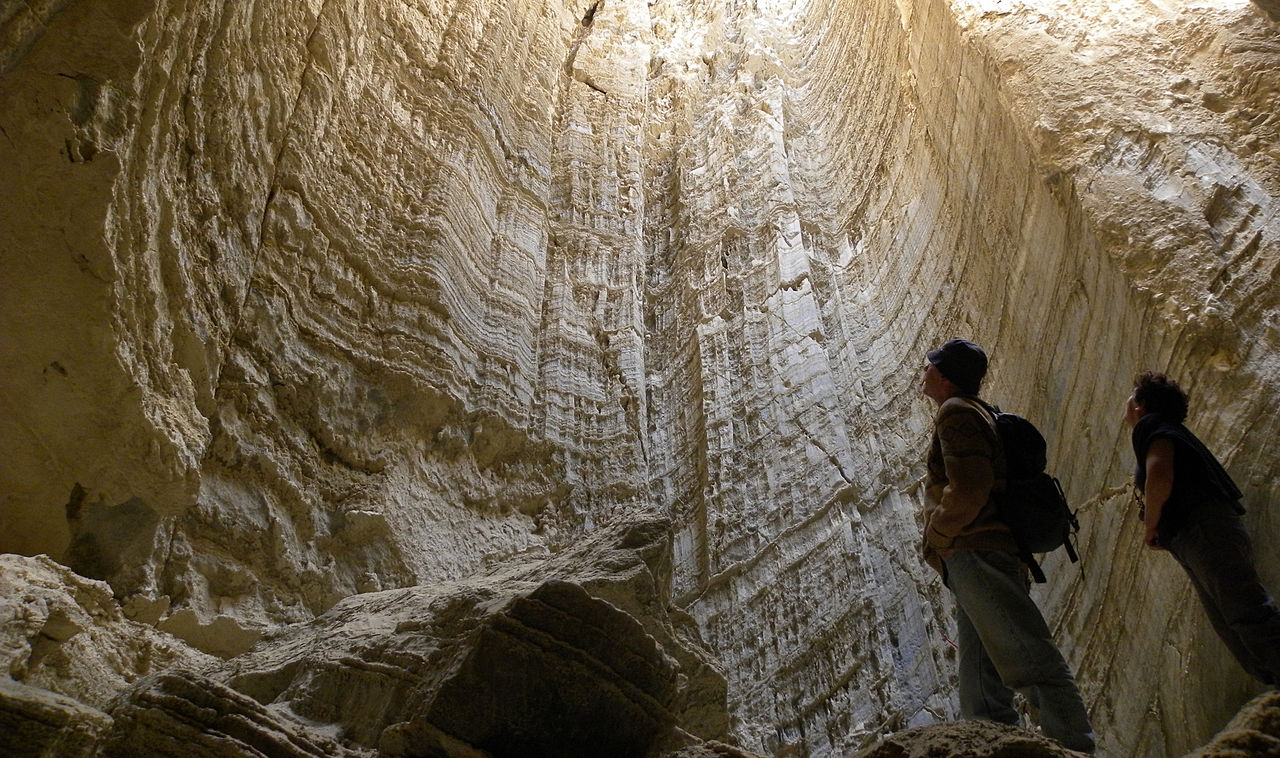
\includegraphics[height=2.8cm,width=1\textwidth,keepaspectratio]{surface_types/salt.jpg}\\
            \caption*{Соляные отложения}
            \label{fig:surface_types/salt}
        \end{subfigure}
        \hfill
        \begin{subfigure}[b]{0.3\textwidth}
            \centering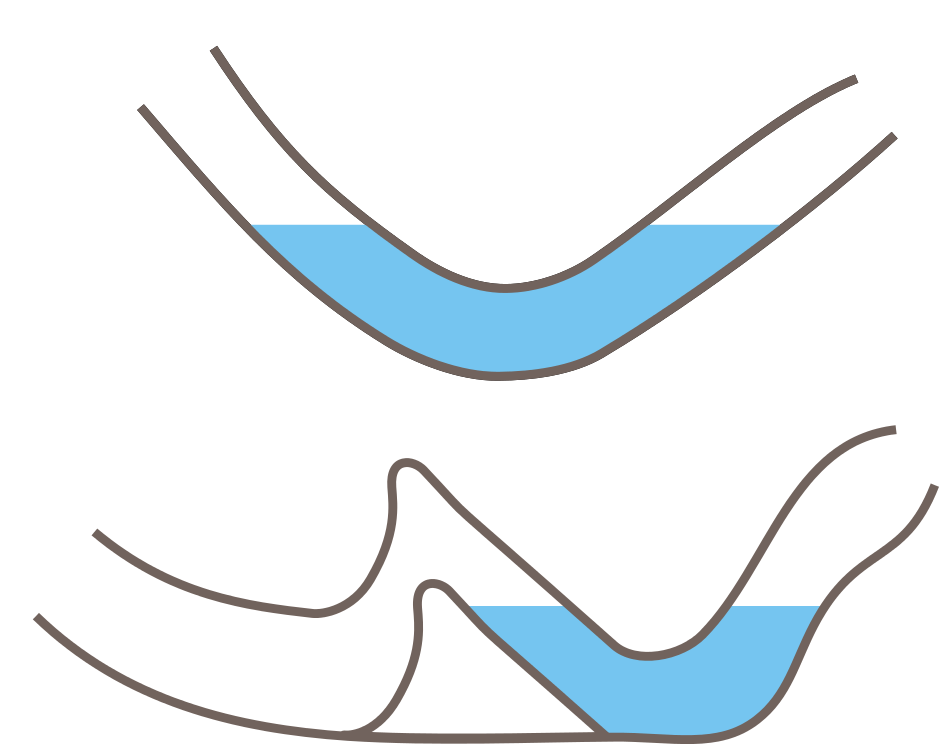
\includegraphics[height=2.8cm,width=1\textwidth,keepaspectratio]{surface_types/siphon.png}\\
            \caption*{Сифоны}
            \label{fig:surface_types/siphon}
        \end{subfigure}
        \hfill
        \begin{subfigure}[b]{0.3\textwidth}
            \centering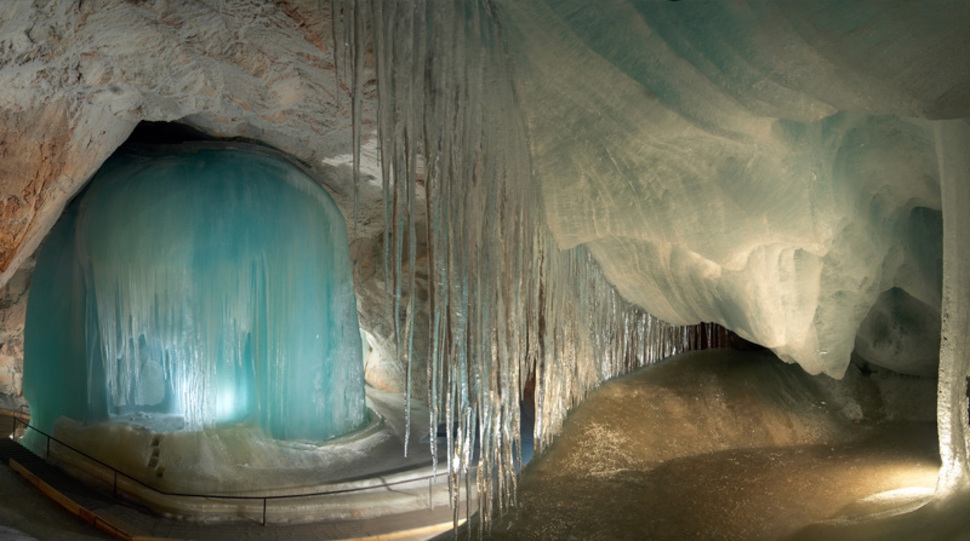
\includegraphics[height=2.8cm,width=1\textwidth,keepaspectratio]{surface_types/ice.png}\\
            \caption*{Ледяные пещеры}
            \label{fig:surface_types/ice}
        \end{subfigure}

        \begin{subfigure}[b]{0.3\textwidth}
            \centering
            \begin{tikzpicture}
                % Include the image in a node
                \node [above right, inner sep=0] (image) at (0,0)
                {\centering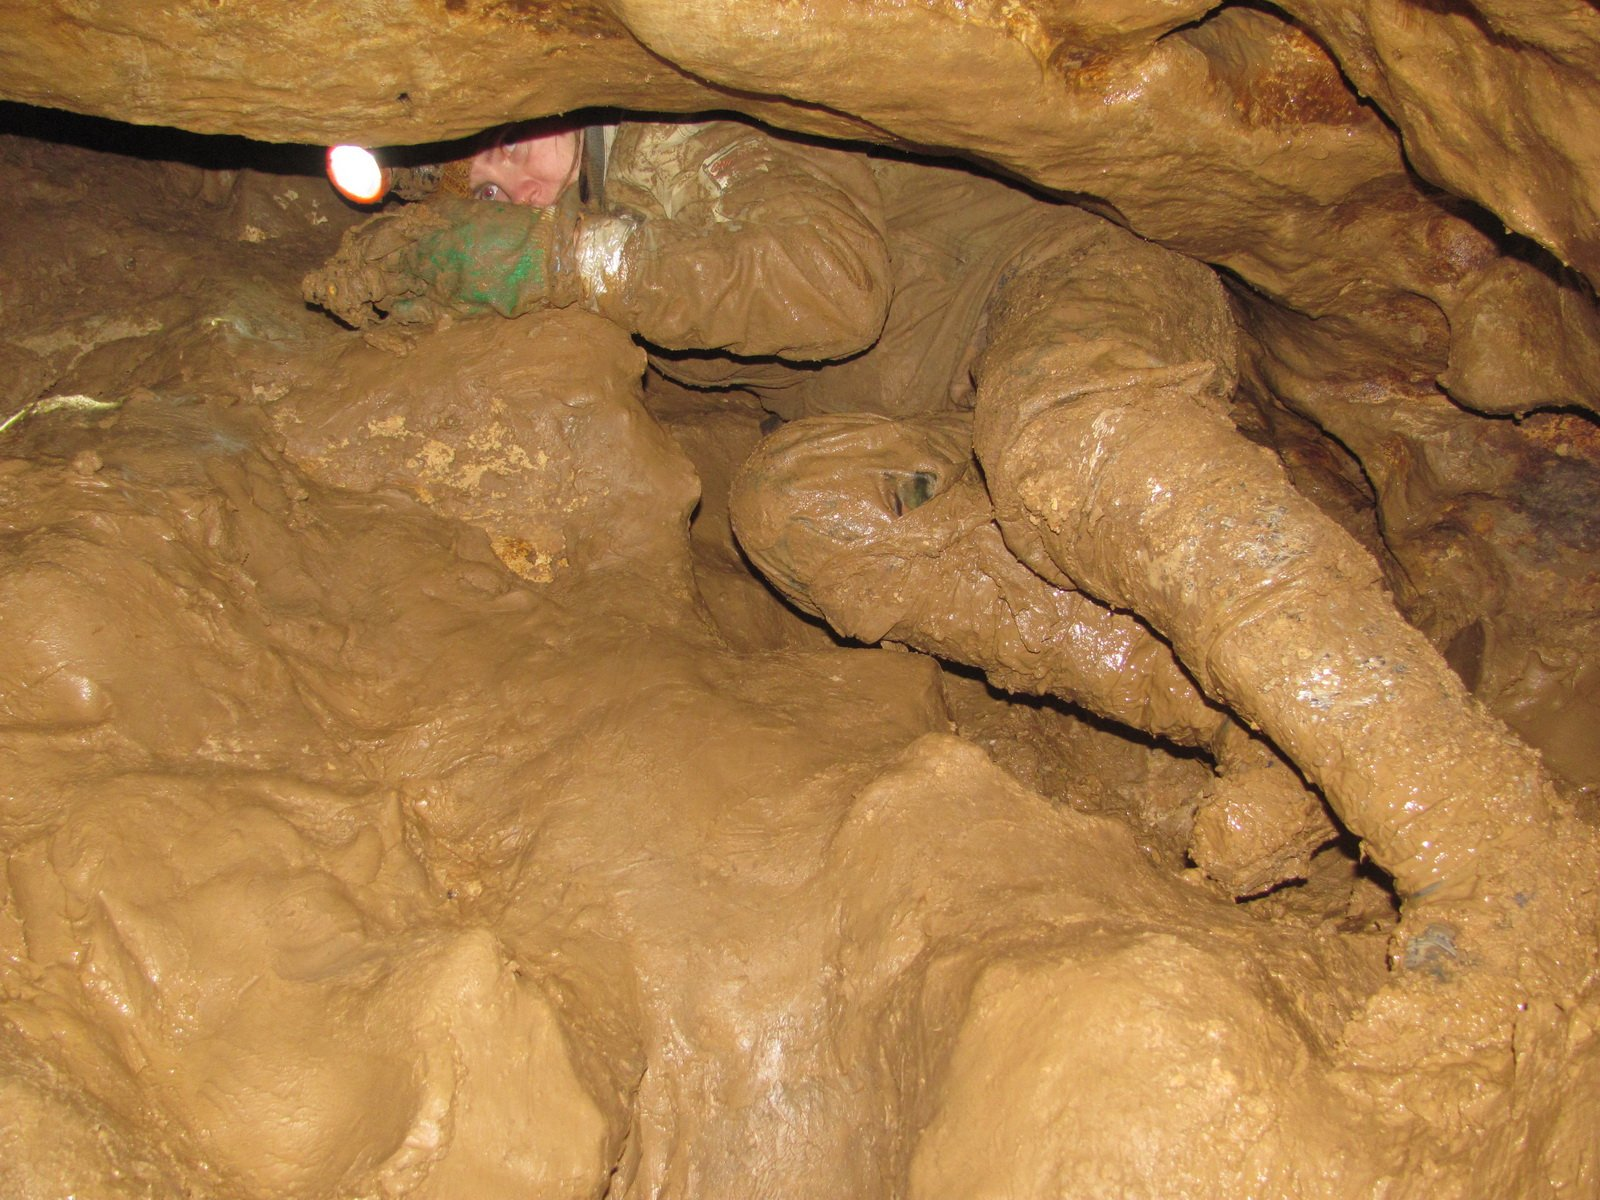
\includegraphics[height=2.8cm,width=1\textwidth,keepaspectratio]{surface_types/clay.jpg}};
                % Create scope with normalized axes
                \begin{scope}[
                        x={($ 0.1*(image.south east)$)},
                        y={($ 0.1*(image.north west)$)}]
                    % Grid and axes' labels
                    % \draw[lightgray,step=1] (image.south west) grid (image.north east);
                    % \foreach \x in {0,1,...,10} { \node [below] at (\x,0) {\x}; }
                    % \foreach \y in {0,1,...,10} { \node [left] at (0,\y) {\y};}
                    % Labels
                    \draw[stealth-, very thick,green] (6,8) -- ++(1,1)
                    node[rounded corners=3pt,right,black,fill=white]{\tiny Human};
                \end{scope}
            \end{tikzpicture}
            \caption*{Глина}
            \label{fig:surface_types/clay.jpg}
        \end{subfigure}
        \hfill
        \begin{subfigure}[b]{0.3\textwidth}
            \centering
            \begin{tikzpicture}
                % Include the image in a node
                \node [above right, inner sep=0] (image) at (0,0)
                {\centering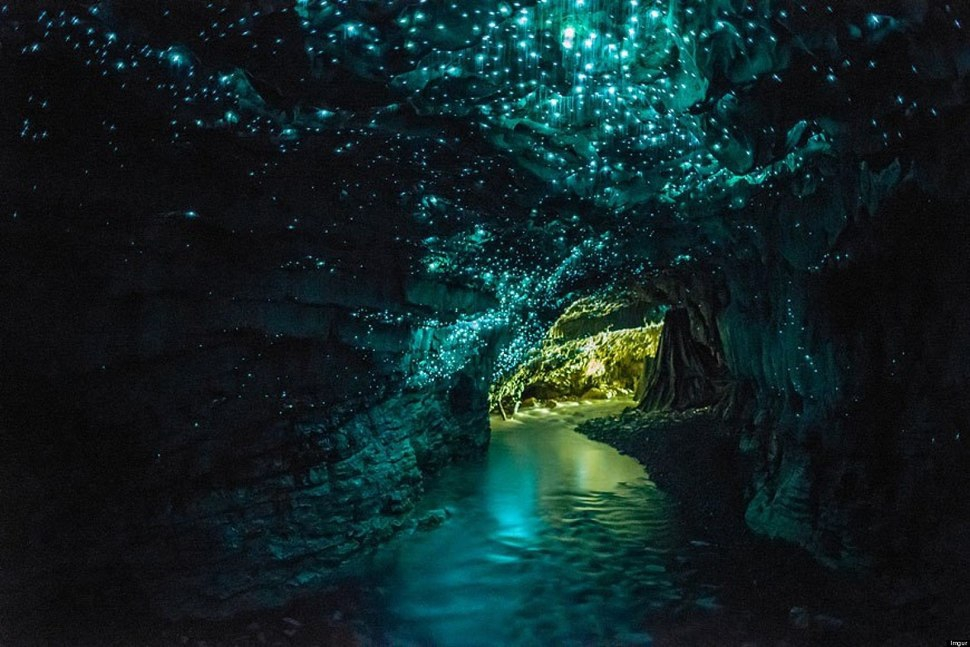
\includegraphics[height=2.8cm,width=1\textwidth,keepaspectratio]{surface_types/splash.png}};
                % Create scope with normalized axes
                \begin{scope}[
                        x={($ 0.1*(image.south east)$)},
                        y={($ 0.1*(image.north west)$)}]
                    % Grid and axes' labels
                    % \draw[lightgray,step=1] (image.south west) grid (image.north east);
                    % \foreach \x in {0,1,...,10} { \node [below] at (\x,0) {\x}; }
                    % \foreach \y in {0,1,...,10} { \node [left] at (0,\y) {\y};}

                    % Labels
                    \draw[stealth-, very thick,green] (5,2) -- ++(-2,+1)
                    node[rounded corners=3pt,left,black,fill=white]{\tiny Puddle};
                \end{scope}
            \end{tikzpicture}
            \caption*{Лужа}
            \label{fig:surface_types/splash.png}
        \end{subfigure}
        \hfill
        \begin{subfigure}[b]{0.3\textwidth}
            \centering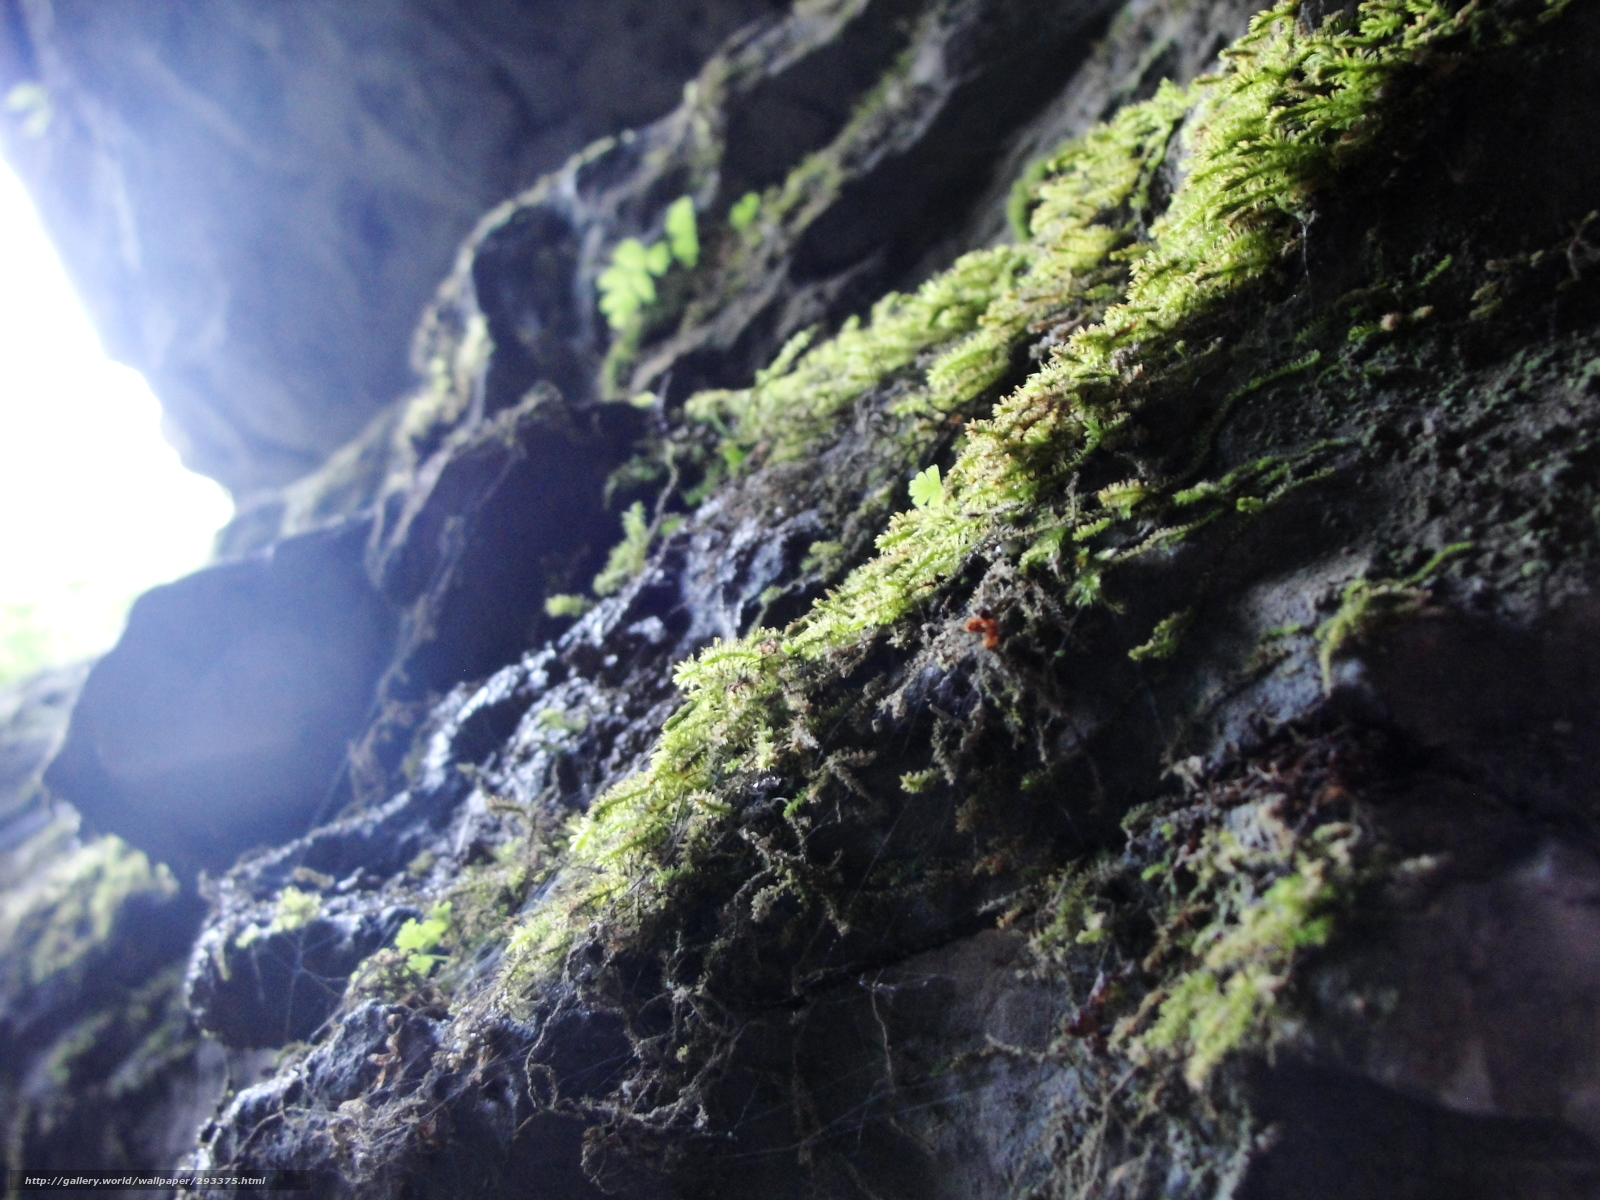
\includegraphics[height=2.8cm,width=1\textwidth,keepaspectratio]{surface_types/moss.jpg}\\
            \caption*{Мох}
            \label{fig:surface_types/moss}
        \end{subfigure}
    \end{figure}
\end{frame}

\begin{frame}[t]{Нерешаемая задача с помощью камеры или лидара}
    \framesubtitle{Вопрос: Как картографировать поверхность под лужей?}
    \vspace{-1cm}
    \begin{columns}[T,onlytextwidth]
        \begin{column}{0.55\textwidth}


            \begin{figure}[H]
                \centering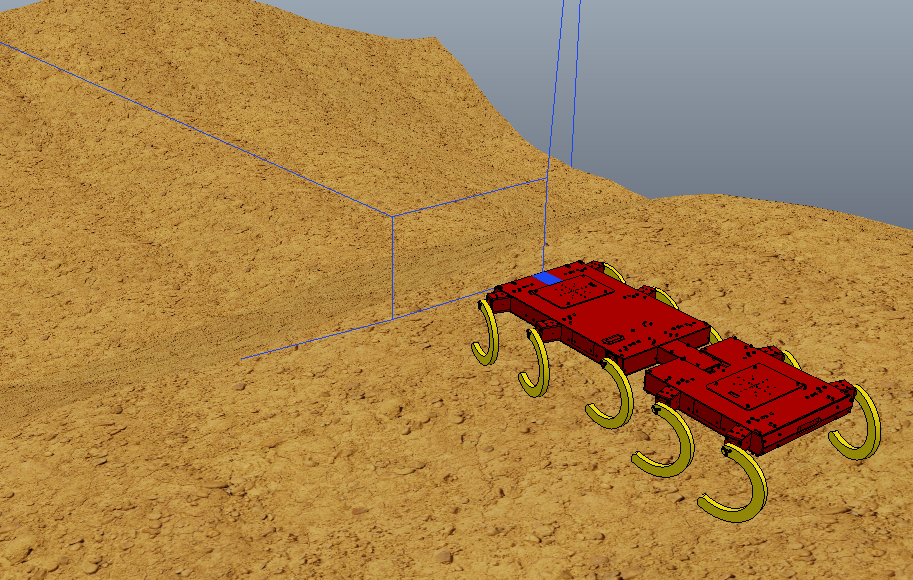
\includegraphics[height=6cm,width=1\textwidth,keepaspectratio]{terrain_wo_water.png}
                \caption*{Поверхность без воды}
            \end{figure}
        \end{column}
        \begin{column}{0.44\textwidth}
            \begin{figure}[H]
                \begin{subfigure}[b]{0.9\textwidth}
                    \centering
                    \begin{tikzpicture}
                        % Include the image in a node
                        \node [above right, inner sep=0] (image) at (0,0)
                        {\centering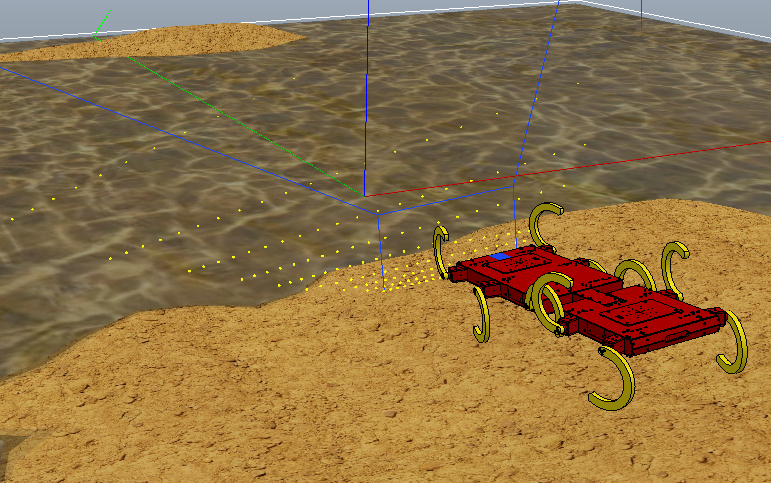
\includegraphics[height=3.5cm,width=1\textwidth,keepaspectratio]{terrain_w_water1.png}};
                        % Create scope with normalized axes
                        \begin{scope}[
                                x={($ 0.1*(image.south east)$)},
                                y={($ 0.1*(image.north west)$)}]
                            % Grid and axes' labels
                            % \draw[lightgray,step=1] (image.south west) grid (image.north east);
                            % \foreach \x in {0,1,...,10} { \node [below] at (\x,0) {\x}; }
                            % \foreach \y in {0,1,...,10} { \node [left] at (0,\y) {\y};}
                            % Labels
                            \draw[stealth-, very thick,green] (6,8) -- ++(2,1)
                            node[rounded corners=3pt,right,black,fill=white]{\tiny Water};

                            \draw[stealth-, very thick,green] (0.5,5.5) -- (3,2);
                            \draw[stealth-, very thick,green] (2.5,4.2) -- (3,2);
                            \draw[stealth-, very thick,green] (4.5,4) -- (3,2)
                            node[rounded corners=3pt,below,black,fill=white]{\tiny Lidar data};
                        \end{scope}
                    \end{tikzpicture}
                    % \caption*{}
                    \label{fig:terrain_w_water1.png}
                \end{subfigure}
                \vspace{-0.5cm}

                \begin{subfigure}{0.8\textwidth}
                    \centering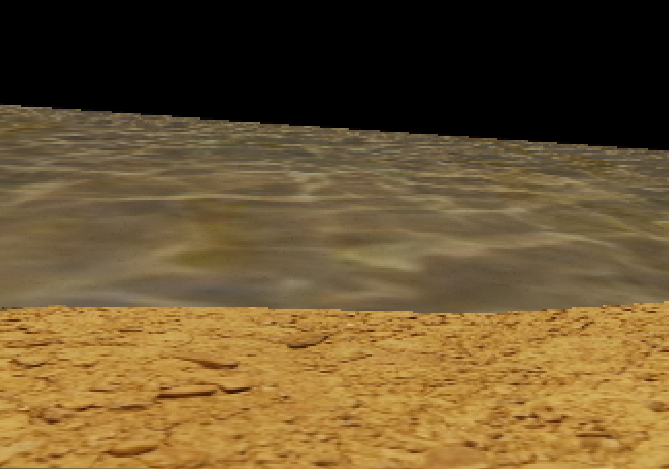
\includegraphics[height=2cm,width=1\textwidth,keepaspectratio]{terrain_w_water_camera.png}
                    \caption*{Вид с камеры}
                \end{subfigure}
            \end{figure}
        \end{column}
    \end{columns}

\end{frame}

% \begin{frame}[t]{Problem statement}
%     \framesubtitle{}
%     \begin{columns}[T,onlytextwidth]
%         \begin{column}{0.45\textwidth}
%             \begin{block}{Problem 1}
%                 How to obtain a useful information about terrain, \textbf{when we have a SLAM based on lidars, cameras}?
%                 \vspace{5pt}

%                 \uncover<2->{\alert{\large Obtain map and type of terrain}}
%             \end{block}
%         \end{column}
%         \begin{column}{0.45\textwidth}
%             \begin{block}{Problem 2}
%                 How to obtain a useful information about terrain,\textbf{ when main navigation system died}?
%                 \vspace{5pt}

%                 \uncover<2->{\alert{\large Problem 1 + localization}}
%             \end{block}
%         \end{column}
%     \end{columns}
% \end{frame}

\begin{frame}[t]{Постановка проблемы}
    \framesubtitle{}
    \begin{block}{Проблема 1}
        \large
        Как получить \underline{полезную информацию} о поверхности, \textbf{когда имеется решенная навигация}?
        \vspace{5pt}

        \uncover<2->{\alert{\large Карта местности и тип поверхности}}
    \end{block}
\end{frame}

\begin{frame}[t]{Предлагаемое решение}
    \framesubtitle{}
    \begin{exampleblock}{Проблема 1}
        \large
        \textit{Карта может быть построена}, \textbf{используя датчики силы} на каждой ноге робота, получив \textbf{плотное облако точек}. Облако точек генерируется из построенной полигональной сетки с помощью \textbf{модифицированной 2D триангуляции Делоне}. Полигональная сетка основана на точках касания ног поверхности.
        \vspace{5pt}

        \textit{Тип поверхности} может быть получен с помощью решения задачи \textbf{классификация поверхности}, используя \textbf{Машинное Обучение}.
    \end{exampleblock}
\end{frame}

% \begin{frame}[t]{Proposed solutions}
%     \framesubtitle{}
%     \begin{columns}[T,onlytextwidth]
%         \begin{column}{0.45\textwidth}
%             \begin{exampleblock}{Problem 1}
%                 \textit{Map can be built} \textbf{using tactile sensors} on each leg of the robot and create a \textbf{dense point cloud} using sampling from generated mesh using \textbf{modified Delaunay triangulation}.
%                 \vspace{5pt}

%                 \textit{Terrain type} can be obtained solving \textbf{Определение типа поверхности} problem using \textbf{machine learning}.
%             \end{exampleblock}
%         \end{column}
%         \begin{column}{0.45\textwidth}
%             \begin{exampleblock}{Problem 2}
%                 \textit{Localization problem} can be solved by \textbf{fused data} from net of \textbf{beacons} plus \textbf{several IMU} on board and knowing a \textbf{kinematics} of the system.
%             \end{exampleblock}
%         \end{column}
%     \end{columns}
% \end{frame}



\begin{frame}[t]{Литературный обзор}
    \framesubtitle{}
    \vspace{-0.3cm}
    \large
    Рассмотренные проблемы:
    \vspace{-0.1cm}
    \begin{itemize}
        \item Пещеры: препятствия, размеры.
        \item Роботы для исследования пещер: от дирижаблей, до шагающих.
        \item Методы построения карты: оптические и тактильные.
    \end{itemize}
    \vspace{-0.2cm}

    \begin{block}{Существующие проблемы}
        \begin{itemize}
            \item Робототехнические системы для исследования свободных пещер
            \item Построение поверхности с помощью датчика силы на манипуляторе
            \item Построение карты с помощью лидаров и камер
        \end{itemize}
    \end{block}
    \vspace{-0.2cm}

    \only<2>{\centering\alert{Найдена нерешенная проблема}}
\end{frame}

\begin{frame}[t]{Разработка робота}
    \framesubtitle{Требования к роботу}
    \large
    \textbf{Задача} --  выбрать движитель. Робот должен:
    \begin{itemize}
        \item Иметь \textit{малые размеры}, чтобы лазать и не застевать в щелях
        \item Обладать достаточной \textit{проходимостью} для преодоления сыпучих грунтов
        \item Преодолевать \textit{небольшие водные препятствия}
        \item Иметь возможнсоть \textit{залезать на большие валуны}
    \end{itemize}
    \uncover<2->{\large\centering\alert{Шагающий цикловой движитель с 1 степенью свободы в ноге}}
\end{frame}

\begin{frame}[t]{Разработка робота}
    \framesubtitle{Структурный синтез}
    \only<1-2>{\large\begin{block}{Вопрос}
            Какое оптимальное количество ног должен иметь такой движитель?
        \end{block}}
    \only<2>{\large\begin{alertblock}{Ответ}
            \centering Робот с таким движителем должен иметь \textbf{8---14 ног}!
        \end{alertblock}}
\end{frame}

\begin{frame}[c]{Разработка робота}
    \framesubtitle{Используемые технологии}
    \vspace{-0.9cm}
    \begin{figure}[H]
        \begin{subfigure}[t]{0.32\textwidth}
            \centering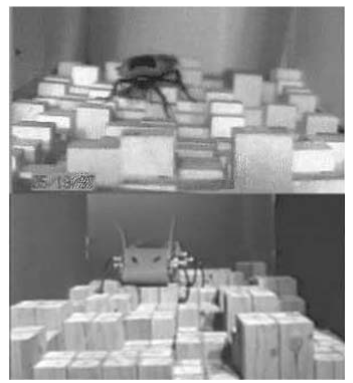
\includegraphics[height=4cm,width=1\textwidth,keepaspectratio]{c1_paper.png}
            \caption*{\small Генерация поверхности \\ (Робот проходит по параметризованной \textbf{искусственной территории})}
        \end{subfigure}
        \hfill
        \begin{subfigure}[t]{0.32\textwidth}
            \centering
\includegraphics[height=4cm,width=1\textwidth,keepaspectratio]{gazebo_logo.png}
            \caption*{Робототехнический симулятор}
        \end{subfigure}
        \hfill
        \begin{subfigure}[t]{0.32\textwidth}
            \centering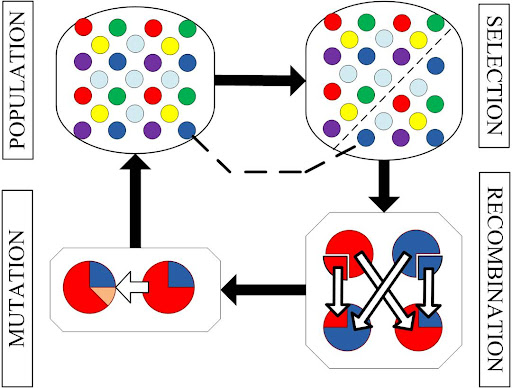
\includegraphics[height=5.5cm,width=1\textwidth,keepaspectratio]{gen_algo.jpg}
            \caption*{Генетический алгоритм \\ (OpenAI-ES)}
        \end{subfigure}
        \hfill
    \end{figure}
\end{frame}

\begin{frame}[t]{Разработка робота}
    \framesubtitle{Предположения}
    \large
    \begin{itemize}
        \item Сгенерированное семейство с одинаковыми константами имеет ту же сложность. 
        \\ 
        Парметры для генерации:
              \begin{itemize}
                \large
                  \item Длина и ширина ячейки
                  \item Диапазон высот ячейки
                  \item Закон распределения
              \end{itemize}
              % \item We can generate 
    \end{itemize}
\end{frame}

\begin{frame}[t]{Разработка робота}
    \framesubtitle{Предлагаемое решение}
    \begin{columns}[T,onlytextwidth]
        \begin{column}{0.48\textwidth}
            \begin{figure}[H]
                \centering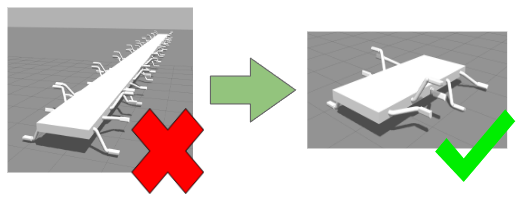
\includegraphics[height=3cm,width=1\textwidth,keepaspectratio]{optimization_idea.png}
                \caption*{\textbf{Идея}: Минимизировать кол-во ног без потери проходимости}
                \label{fig{optimization_idea.png}}
            \end{figure}
        \end{column}
        \begin{column}{0.50\textwidth}
            \vspace{-2cm}
            \begin{figure}[H]
                \centering
                \begin{tikzpicture}
                    % Include the image in a node
                    \node [above right, inner sep=0] (image) at (0,0)
                    {\centering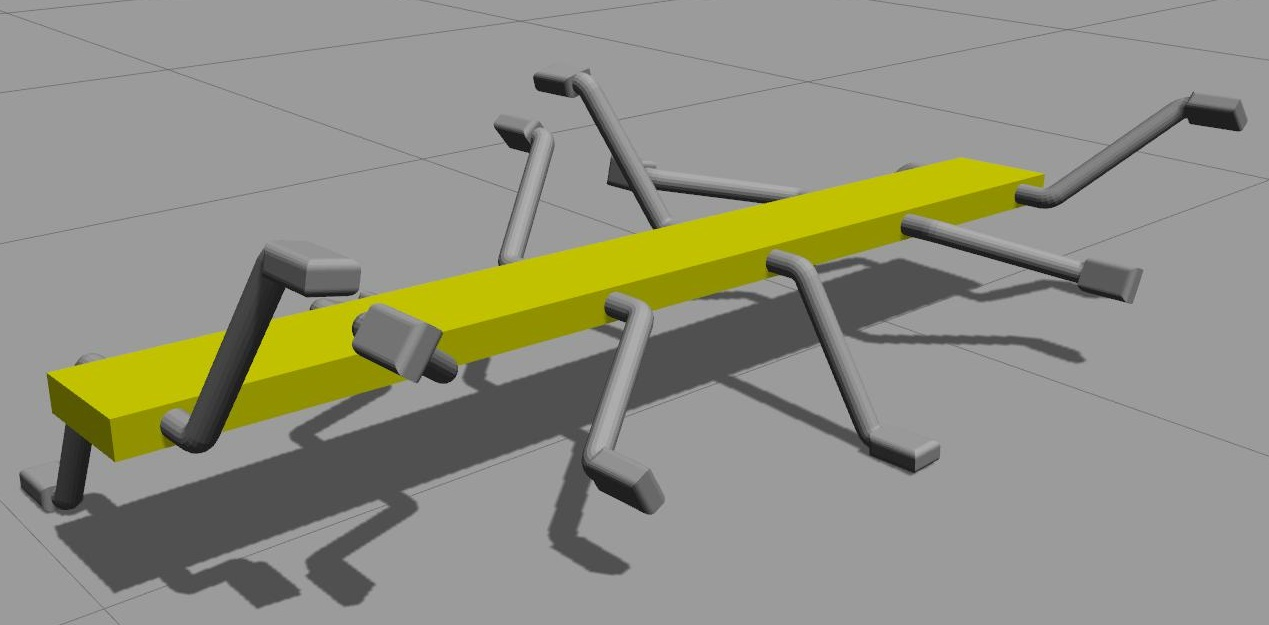
\includegraphics[height=2.5cm,width=1\textwidth,keepaspectratio]{best_gen_robot.jpg}};
                    % Create scope with normalized axes
                    \begin{scope}[
                            x={($ 0.1*(image.south east)$)},
                            y={($ 0.1*(image.north west)$)}]
                        % Grid and axes' labels
                        % \draw[lightgray,step=1] (image.south west) grid (image.north east);
                        % \draw[lightgray,step=0.5] (image.south west) grid (image.north east);
                        % \foreach \x in {0,1,...,10} { \node [below] at (\x,0) {\x}; }
                        % \foreach \y in {0,1,...,10} { \node [left] at (0,\y) {\y};}

                        % Labels
                        \draw [green, very thick,
                            decorate,
                            decoration = {brace,
                                    raise=5pt,
                                    amplitude=5pt,
                                    aspect=0.5}] (1.4,3.6) --  (8.1,6.8)
                        node[rounded corners=3pt, pos=0.5,above left =14pt,black,fill=white]{\tiny $(\gamma - 1) h_{\text{leg}}sin(\alpha)$};

                        \draw[stealth-, very thick,green] (9.5,7.8) -- (7.8,1.94);
                        \draw[stealth-, very thick,green] (1.5,2.8) -- (7,1)
                        node[rounded corners=3pt,right,black,fill=white]{\tiny $\gamma = 6$};

                        \draw[thin,green] (6.7,4) -- (5.75,9);
                        \draw[thin,green] (4.85,3.5) -- (5.75,9);
                        \draw[thin,green,stealth-stealth] (6.32,6) arc (-79.2:-99.2:3) node [rounded corners=3pt,below = 2pt,black,fill=white, midway] {\tiny $\alpha$};
                    \end{scope}
                \end{tikzpicture}
                % \caption*{}
                \label{fig:best_gen_robot.jpg}
            \end{figure}
            \vspace{-1cm}
            {\footnotesize
                \begin{eqnarray*}
                    % \resizebox{0.9\hsize}{!}{
                    F \rightarrow max = \beta \left( {\omega}_{1} \cdot \overbrace{\delta}^{\text{Дистанция}} + {\omega}_{2} \cdot \overbrace{\frac{1}{(\gamma - 1) h_{\text{leg}}sin(\alpha)}}^{\text{Упр. длина корпуса}}\right) +\\ \nonumber + (1 - \beta) {\delta}^{{\omega}_{1}} {\left( \frac{1}{(\gamma - 1)h_{\text{leg}}sin(\alpha)}\right)}^{{\omega}_{2}}
                    % }
                \end{eqnarray*}
            }
            % \vspace{1pt}

            $\beta$ -- адаптивный параметр, \\ ${\omega}_{1,2} \in  [ 0..1 ] $ -- весовые коэффициенты.
        \end{column}
    \end{columns}
\end{frame}

\begin{frame}[t]{Разработка робота}
    \framesubtitle{Видео: История одного сгенерированного робота}
    \vspace{-0.6cm}
    \begin{figure}[H]
        % \href{run:./videos/pass_rand_terr.mp4}{
        \href{https://youtu.be/DcovvkTZgsg}{
            \centering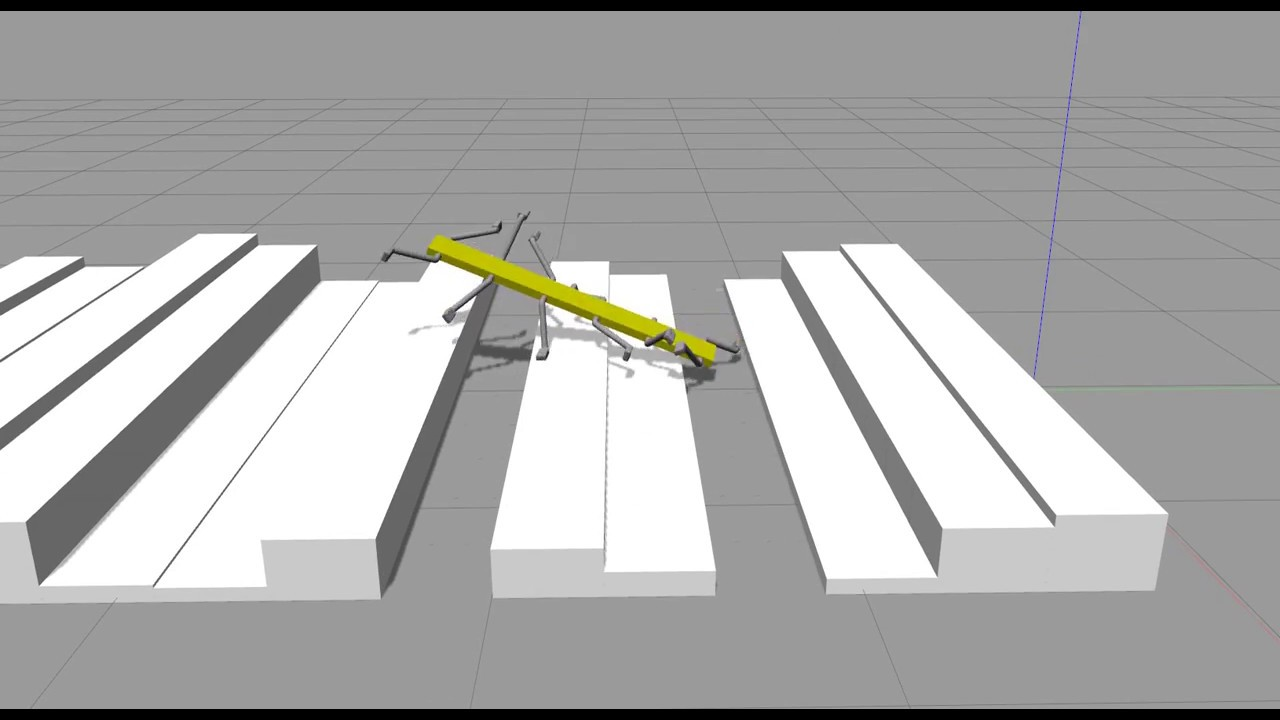
\includegraphics[height=6cm,width=1\textwidth,keepaspectratio]{genetic_video_preview.jpg}}
        % \caption{Click on a picture for a video}
    \end{figure}
\end{frame}

\begin{frame}[t]{Разработка робота}
    \framesubtitle{Конкретные результаты: $\omega_1 = 0.6$, $\omega_2 = 0.4$}
    \vspace{-0.6cm}

    \begin{table}[H]
        \centering
        \begin{tabular}{c|c|c|c|c}
         & \textbf{\begin{tabular}[c]{@{}c@{}}Тип\\ территории\end{tabular}} & \textbf{Кол-во ног} & \textbf{\begin{tabular}[c]{@{}c@{}}Угол между\\ соседними ногами\end{tabular}} & \textbf{Кол-во индивидов} \\
         \hline
         \rule{0cm}{0.5cm}
        \textbf{Этап 1} &  & \cellcolor[HTML]{DAE8FC}12 & 73 & 200 \\ \cline{1-1} \cline{3-5} 
         & \multirow{-2}{*}{\begin{minipage}{2.5cm}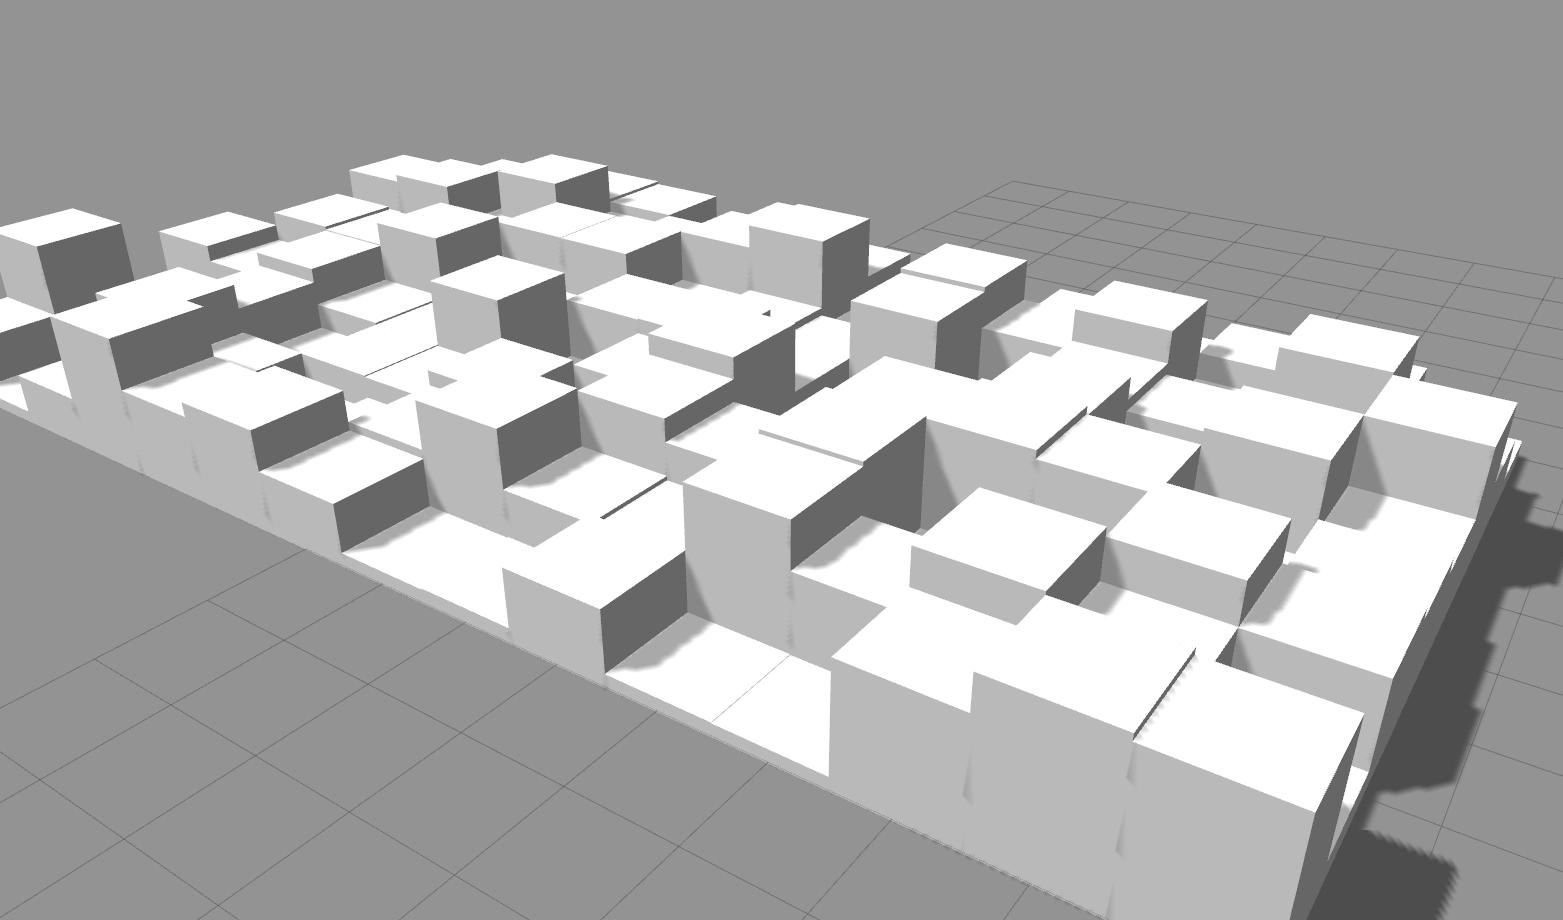
\includegraphics[height=3cm,width=2.5cm,keepaspectratio]{terrain_1.jpg}\end{minipage}} & \cellcolor[HTML]{DAE8FC}12 & 72 &  \\ [0.5cm] \cline{3-4} 
         & \begin{minipage}{2.5cm}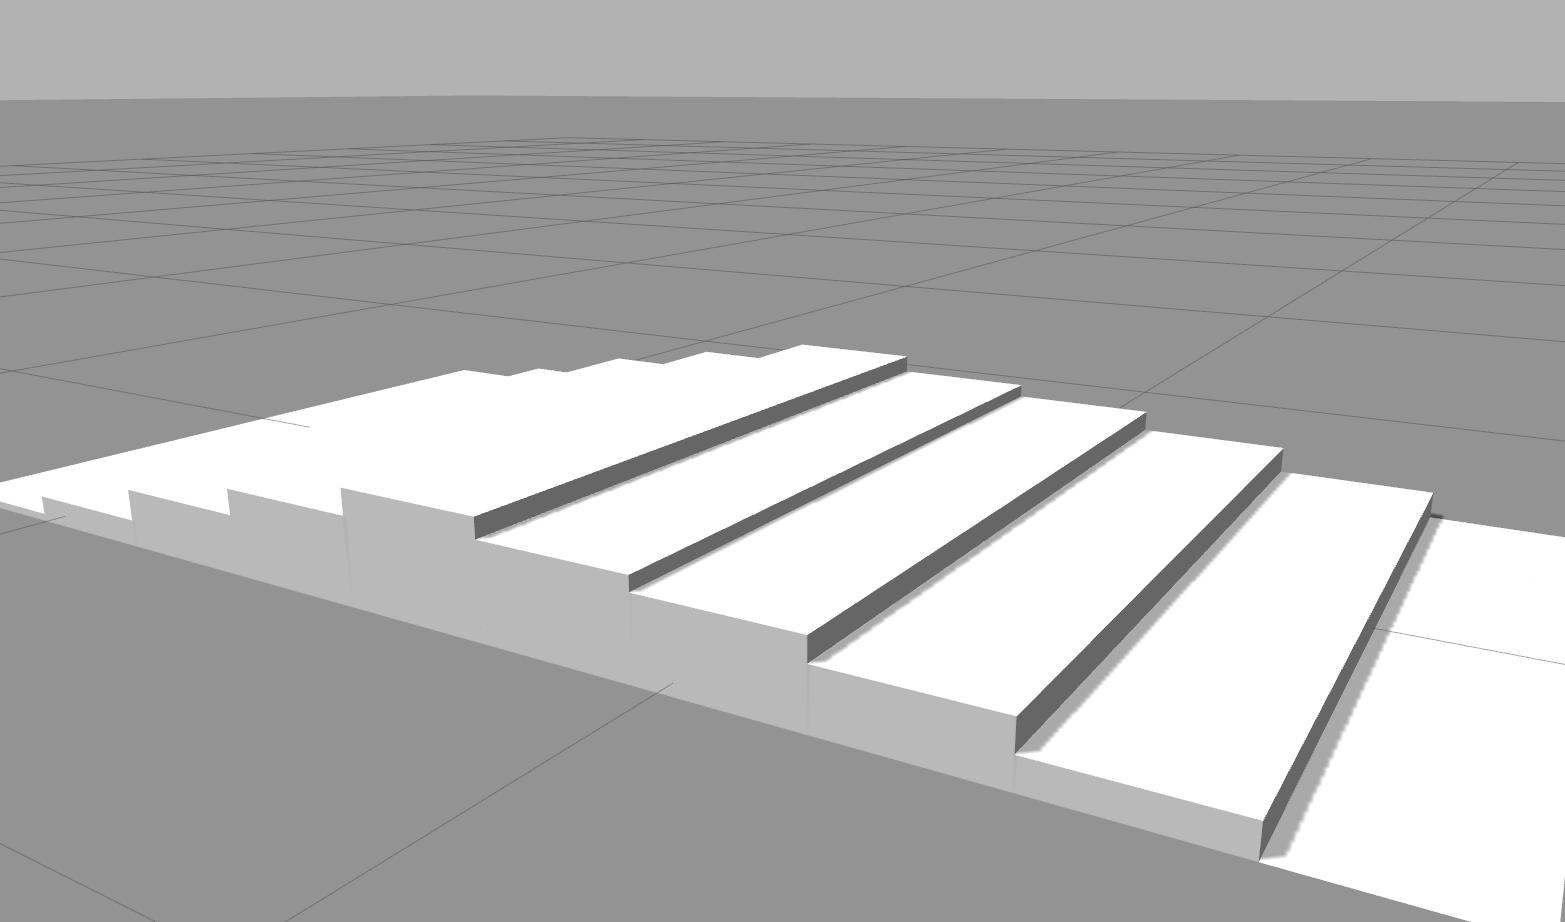
\includegraphics[height=3cm,width=2.5cm,keepaspectratio]{terrain_2.jpg}\end{minipage} & \cellcolor[HTML]{DAE8FC}10 & 68 &  \\ [0.5cm] \cline{3-4}
        \multirow{-3}{*}{\textbf{Этап 2}} & \begin{minipage}{2.5cm}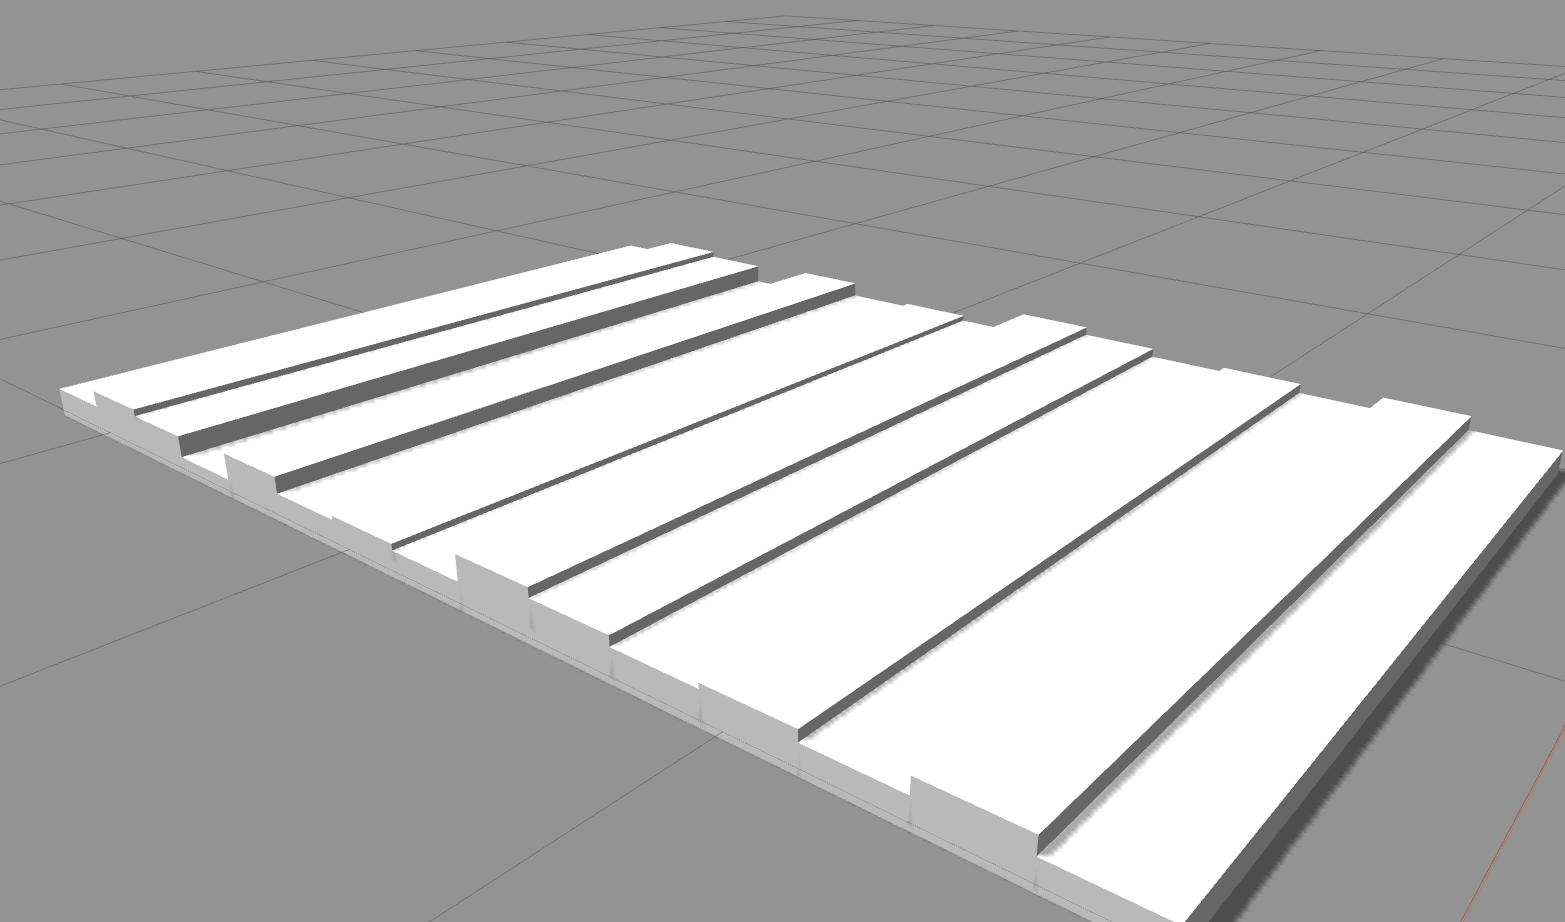
\includegraphics[height=3cm,width=2.5cm,keepaspectratio]{terrain_3.jpg}\end{minipage} & \cellcolor[HTML]{DAE8FC}12 & 77 & \multirow{-3}{*}{55}
        \end{tabular}
        % \caption*{\large\centering\textbf{Summary}: created robot should have 10-12 legs in total}
        \end{table}

\end{frame}

\begin{frame}[t]{Разработка робота}
    \framesubtitle{Закономерность}
    \begin{columns}[T,onlytextwidth]
        \begin{column}{0.49\textwidth}
            Лучшие роботы в экспериментах начинались с 8 до 14 ног для различных значений $\omega$. 
            
            Это объясняется критерием статического равновесия. В таком случае минимум 4 ноги всегда касаются поверхности.    
        \end{column}
        \begin{column}{0.49\textwidth}
            \vspace{-1.8cm}
            \begin{figure}[H]
                \centering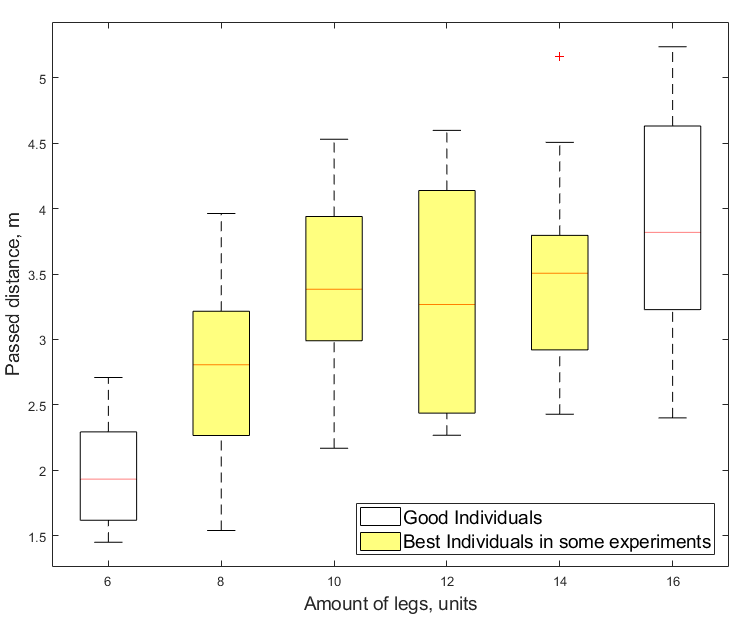
\includegraphics[height=5cm,width=1\textwidth,keepaspectratio]{box_plot_structural_synthesis.png}
                \caption*{Зависимость между кол-вом ног и пройденной дистанцией}
                \label{fig:box_plot_structural_synthesis.png}
            \end{figure}
        \end{column}
    \end{columns}
\end{frame}

\begin{frame}[t]{Разработка робота}
    \framesubtitle{Улучшение проходимости}
    \only<1-2>{\large\begin{block}{Question}
            1. Длинный робот может застрять в щели во время поворота. Как избежать это?

            2. Как залезать на большие уступы?
        \end{block}}
    \only<2>{\large\begin{alertblock}{Answer}
            \centering 1. Добавить возможность двигаться вбок без смены ориентации.

            2. Сделать сегментированное тело.
        \end{alertblock}}
\end{frame}

\begin{frame}[t]{Разработка робота}
    \framesubtitle{Видео}
    \vspace{-0.6cm}
    \begin{figure}[H]
        % \href{run:./videos/sidestep_segments.mp4}{
        \href{https://youtu.be/EQ6oGZVDpoc}{
            \centering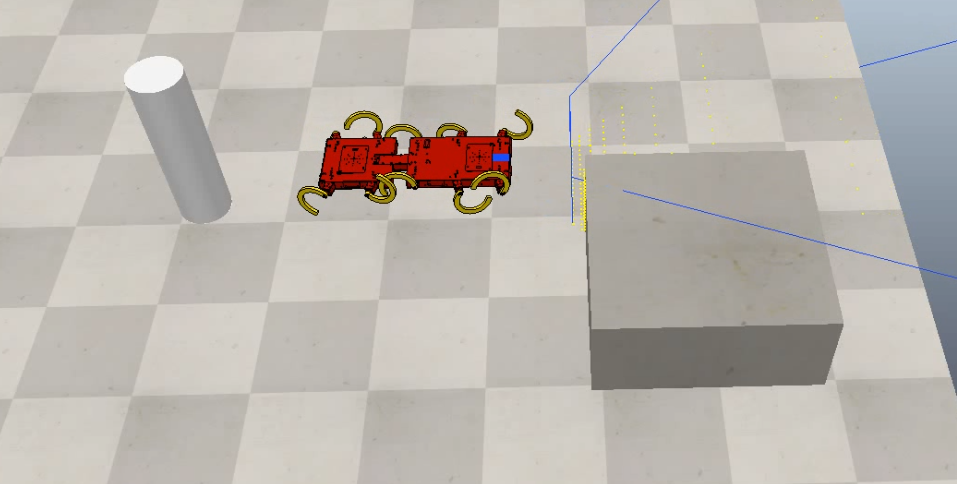
\includegraphics[height=6cm,width=1\textwidth,keepaspectratio]{sidestep_segment_video_preview.png}}
        % \caption{Click on a picture for a video}
    \end{figure}
\end{frame}

\begin{frame}[t]{Разработка робота}
    \framesubtitle{Предлагаемое решение}
    \vspace{-0.8cm}
    \begin{figure}[H]
        \centering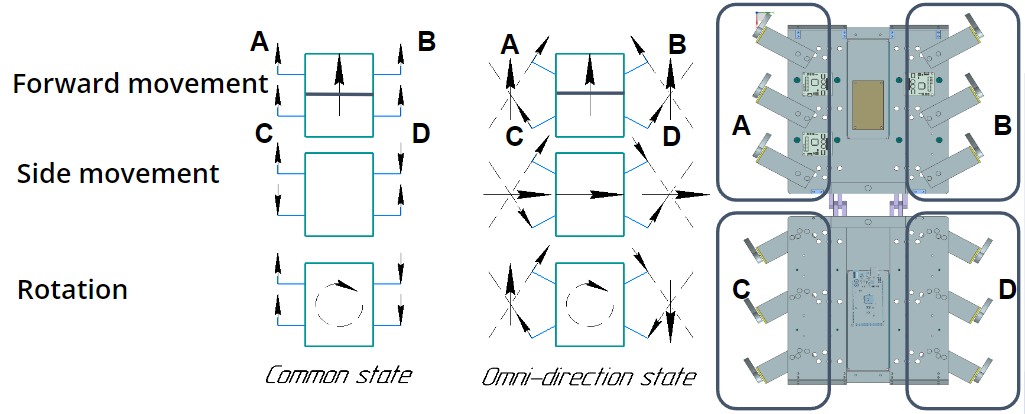
\includegraphics[height=5.5cm,width=1\textwidth,keepaspectratio]{omni_rot.png}
        \caption*{Векторное представление сил в стандартной и всенаправленной компоновке}
    \end{figure}
\end{frame}

\begin{frame}[t]{Разработка робота}
    \framesubtitle{Проботипы робота СтриРус (1)}
    \vspace{-0.7cm}
\begin{table}[H]
    \arrayrulecolor[HTML]{C0C0C0}
    \begin{tiny}
    \begin{tabular}{>{\bfseries}p{1.3 cm}|>{\centering}p{3.5cm}|>{\centering}p{3.5cm}|>{\centering \arraybackslash}p{3.5cm}}
    \multicolumn{1}{p{1.3 cm}}{}  & \multicolumn{1}{p{3.5cm}}{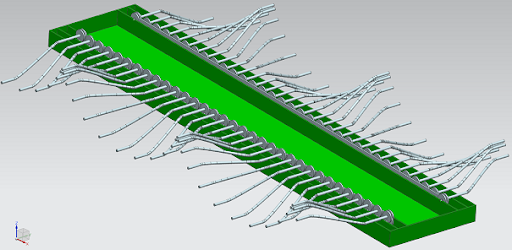
\includegraphics[height=3cm,width=3.5cm,keepaspectratio]{strirus_0.png}}  &  \multicolumn{1}{p{3.5cm}}{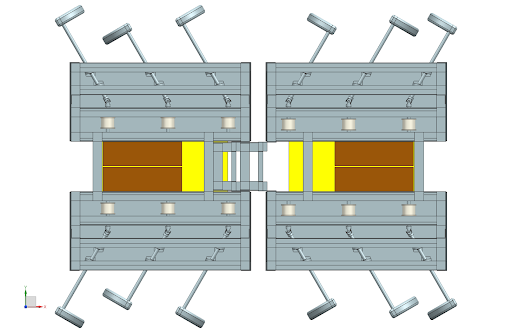
\includegraphics[height=3cm,width=3.5cm,keepaspectratio]{strirus_1.png}} & \multicolumn{1}{p{3.5cm}}{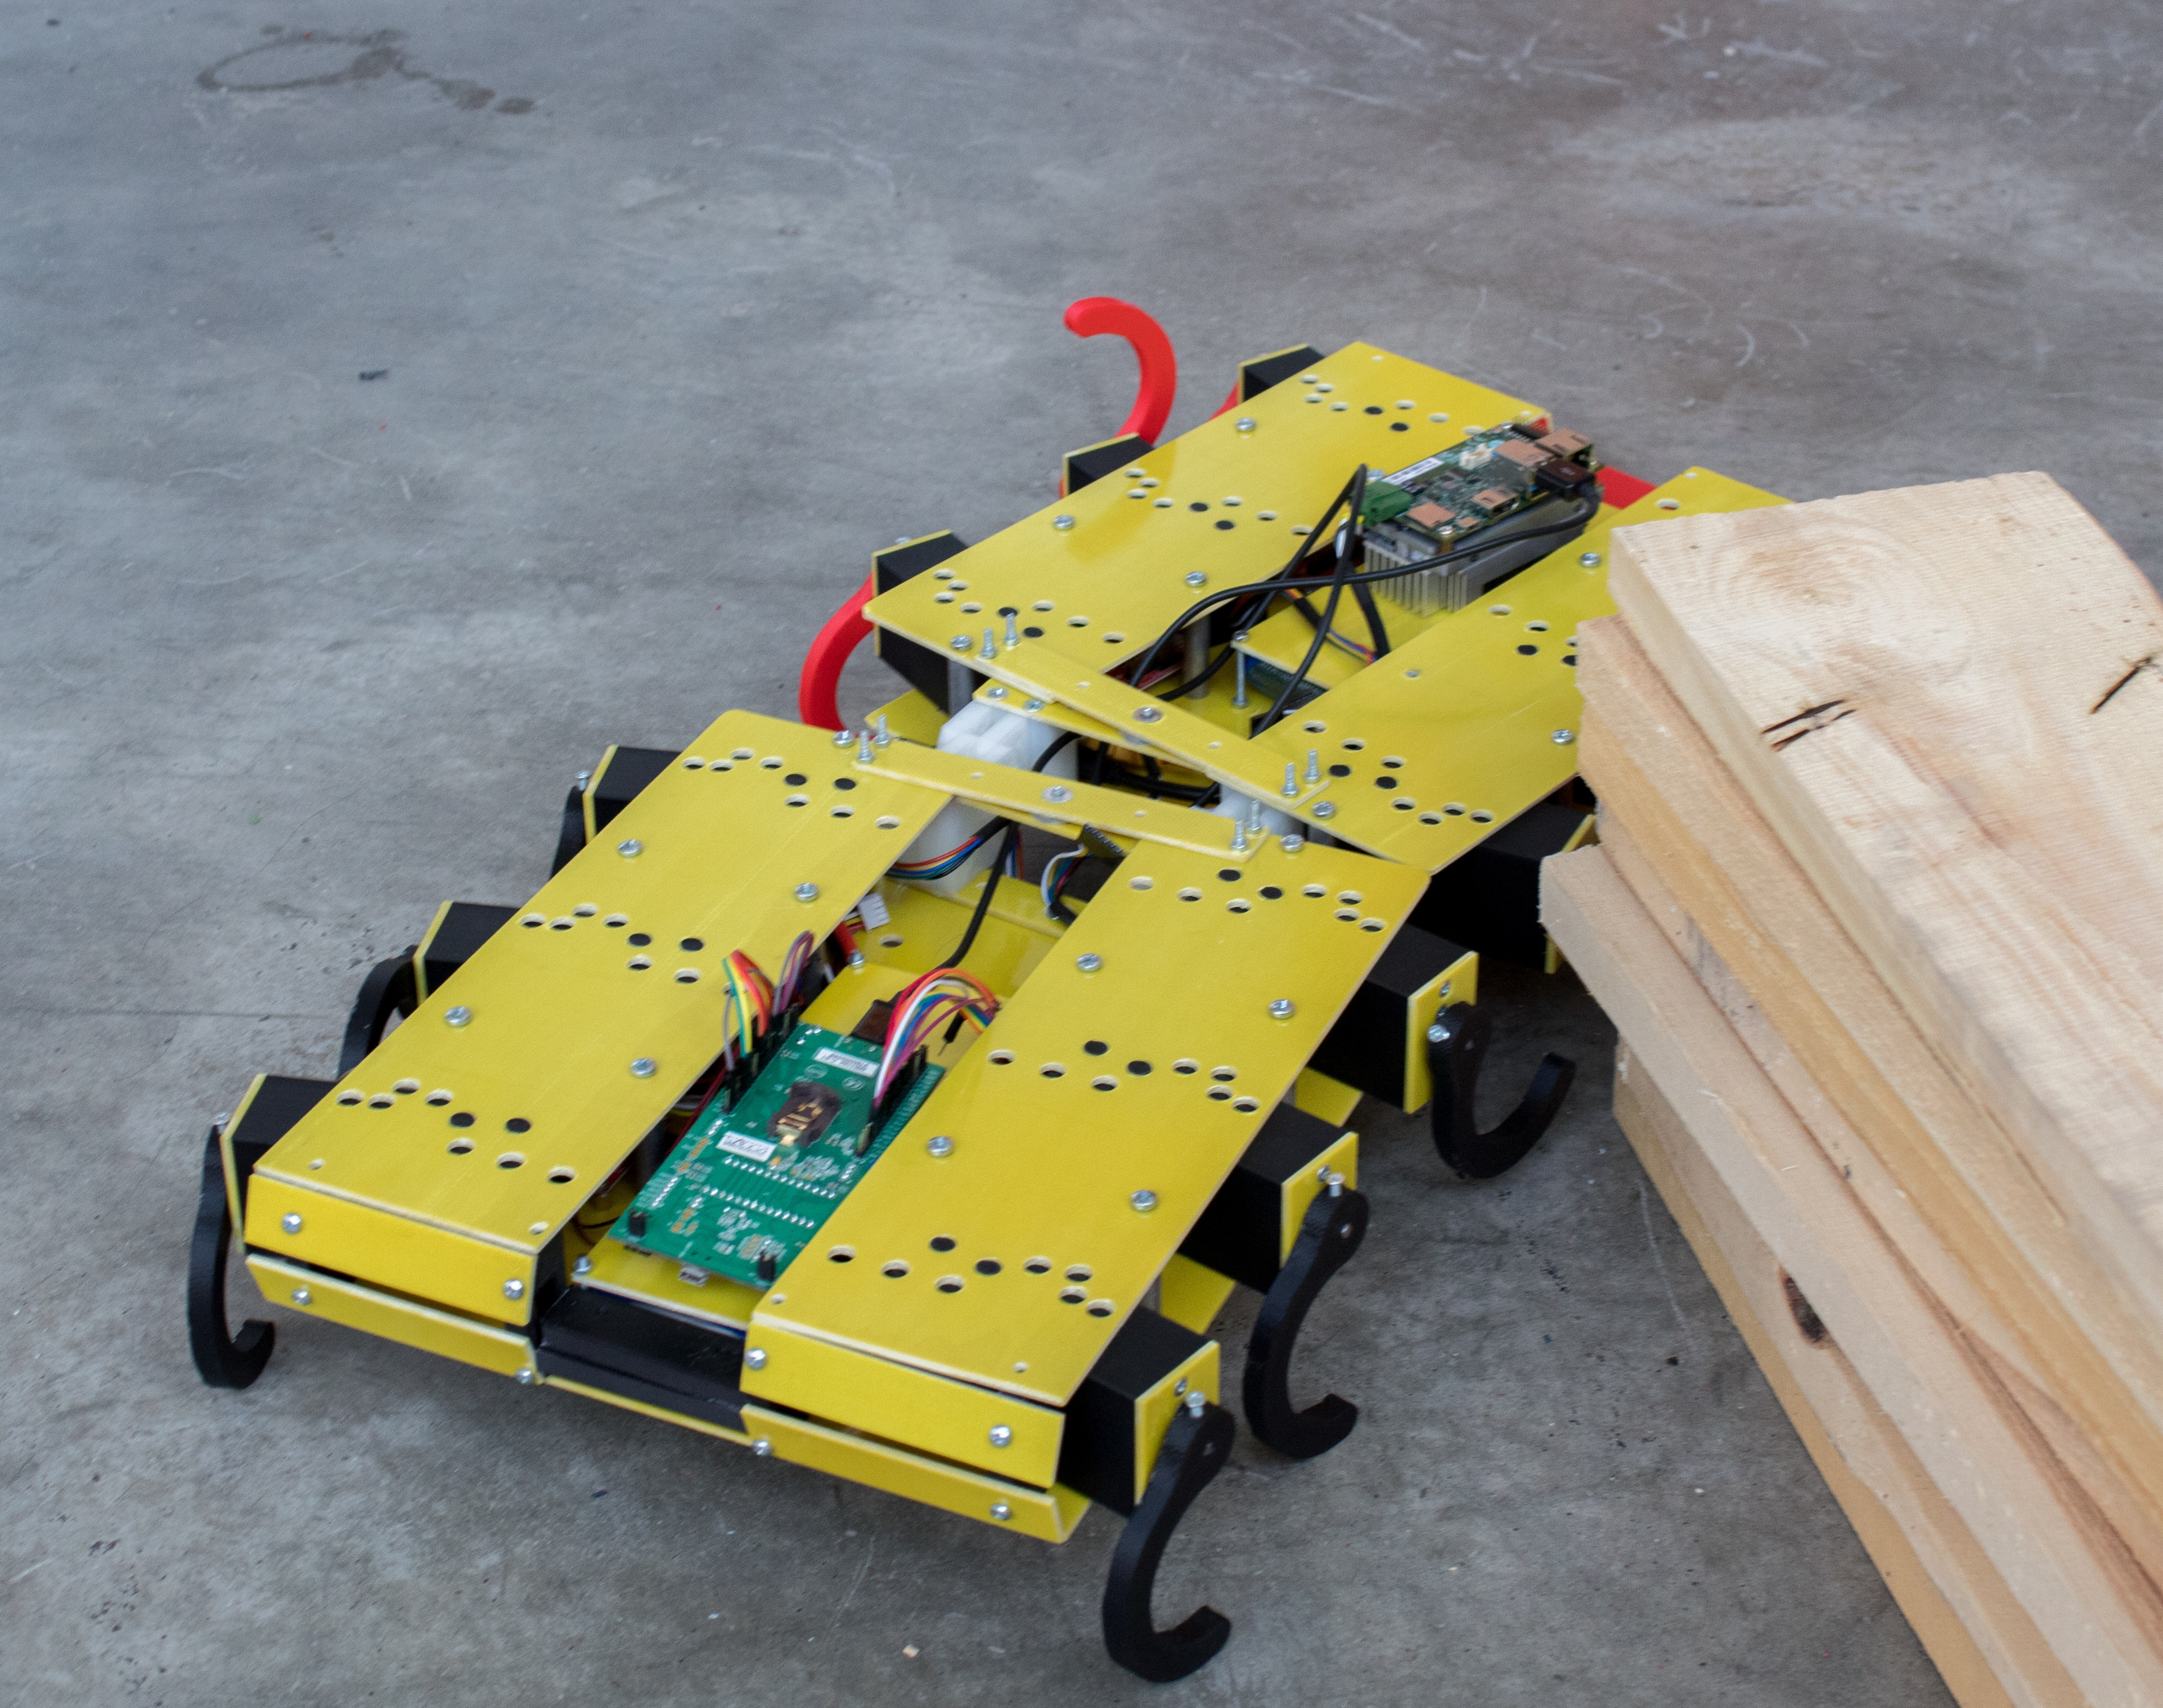
\includegraphics[height=3cm,width=3.5cm,keepaspectratio]{strirus_2.jpg}} \\
     Поколение & 1  & 2 &  3 \\
     \hline
     \rowcolor[HTML]{EFEFEF} 
    Кол-во ног & 54 & 12 & 12 \\ 
     Кол-во сегм. & 1 & 2 & 2 \\
     \rowcolor[HTML]{EFEFEF} 
     Соед. узел & --- & Тангаж & Тангаж, Рыскание \\
    \makecell[l]{Отн. угол \\ нога-тело, град} & 0 & 0--45 & 0, 15, 30, 45 \\
    \rowcolor[HTML]{EFEFEF} 
     Высота ноги, мм & 54 & 60 & 60 \\
     Особенности & Волноход & Непрерывный механизм & 2 DoF у соед. узла \\
    \rowcolor[HTML]{EFEFEF} 
     Недостатки &  \makecell[l]{-- Невозможно установить датчики силы \\ -- Малый КПД} & \makecell[l]{ -- Сложный механизм изм. угла} & \makecell[l]{ -- Маленькие ноги \\ -- Бесполезная возможность рыскания} \\
    \end{tabular}
    \end{tiny}
    \end{table}

\end{frame}

\begin{frame}[t]{Разработка робота}
    \framesubtitle{Проботипы робота СтриРус (2)}
    \vspace{-0.7cm}
    \begin{table}[H]
        \arrayrulecolor[HTML]{C0C0C0}
        \begin{tiny}
        \begin{tabular}{>{\bfseries}p{1.3 cm}|>{\centering}p{3.5cm}|>{\centering \arraybackslash}p{3.5cm}}
        \multicolumn{1}{p{1.3 cm}}{}  & \multicolumn{1}{p{3.5cm}}{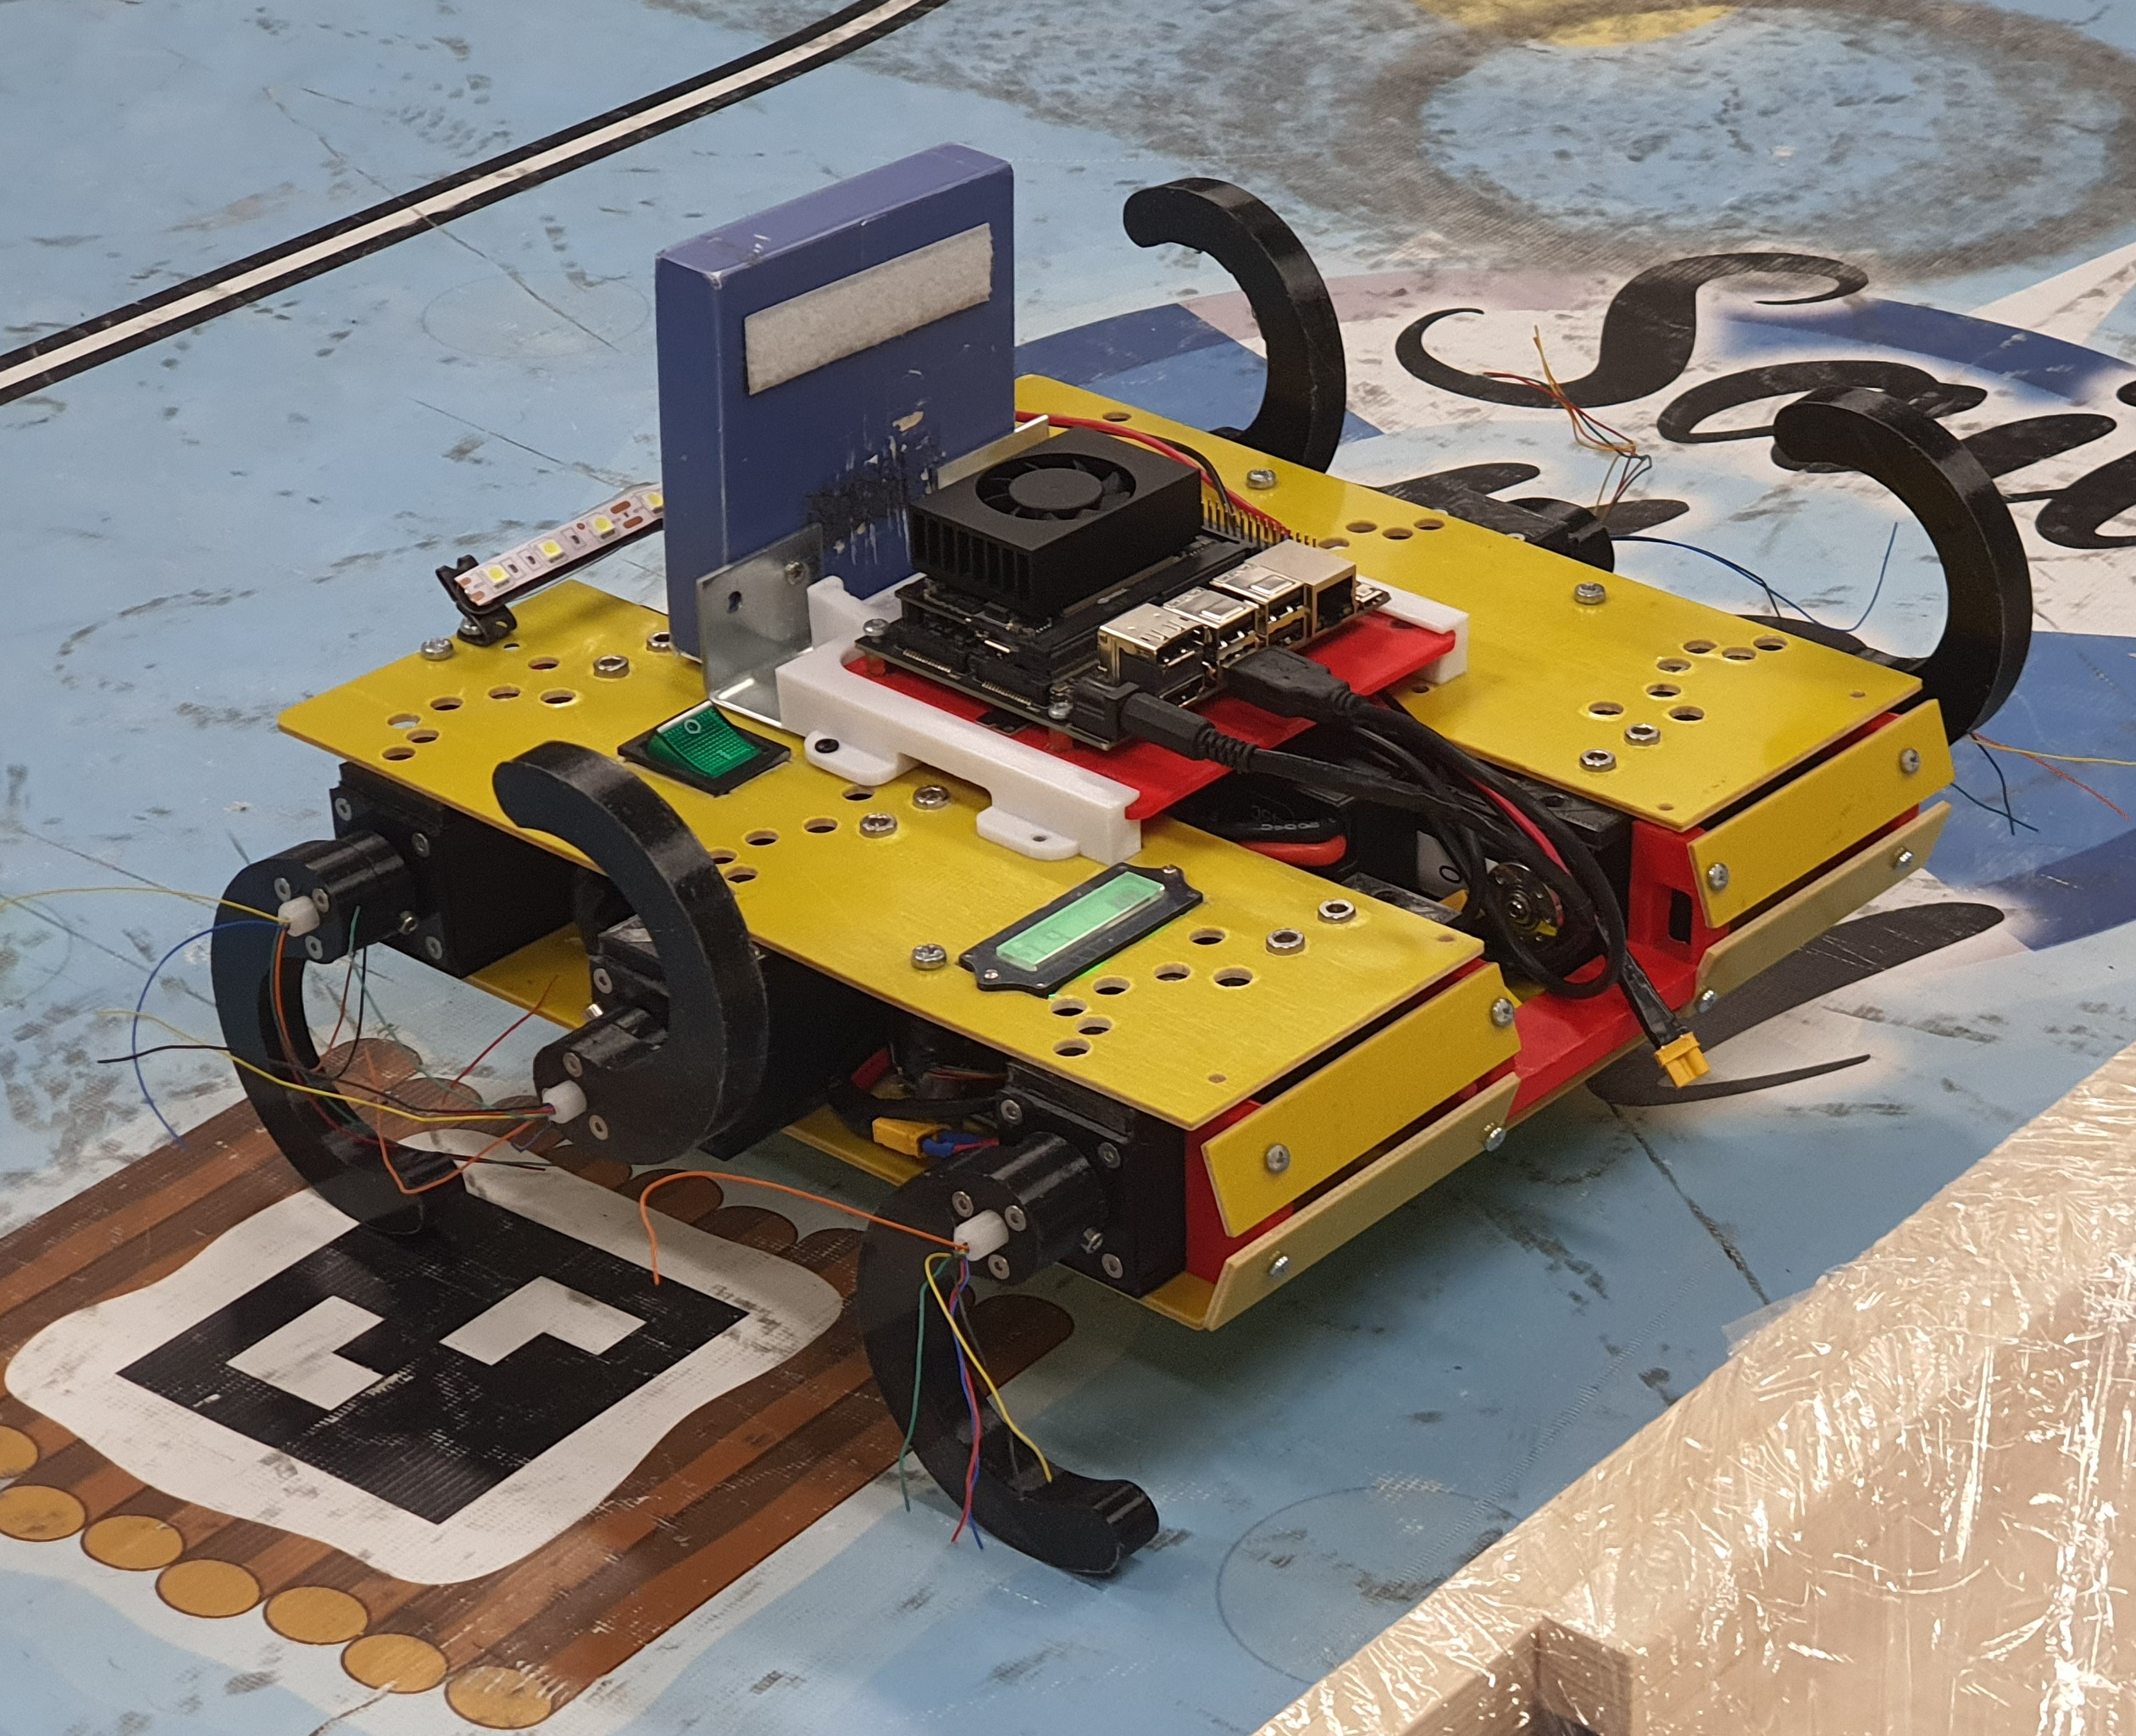
\includegraphics[height=3cm,width=3.5cm,keepaspectratio]{strirus_3.JPG}}  &  \multicolumn{1}{p{3.5cm}}{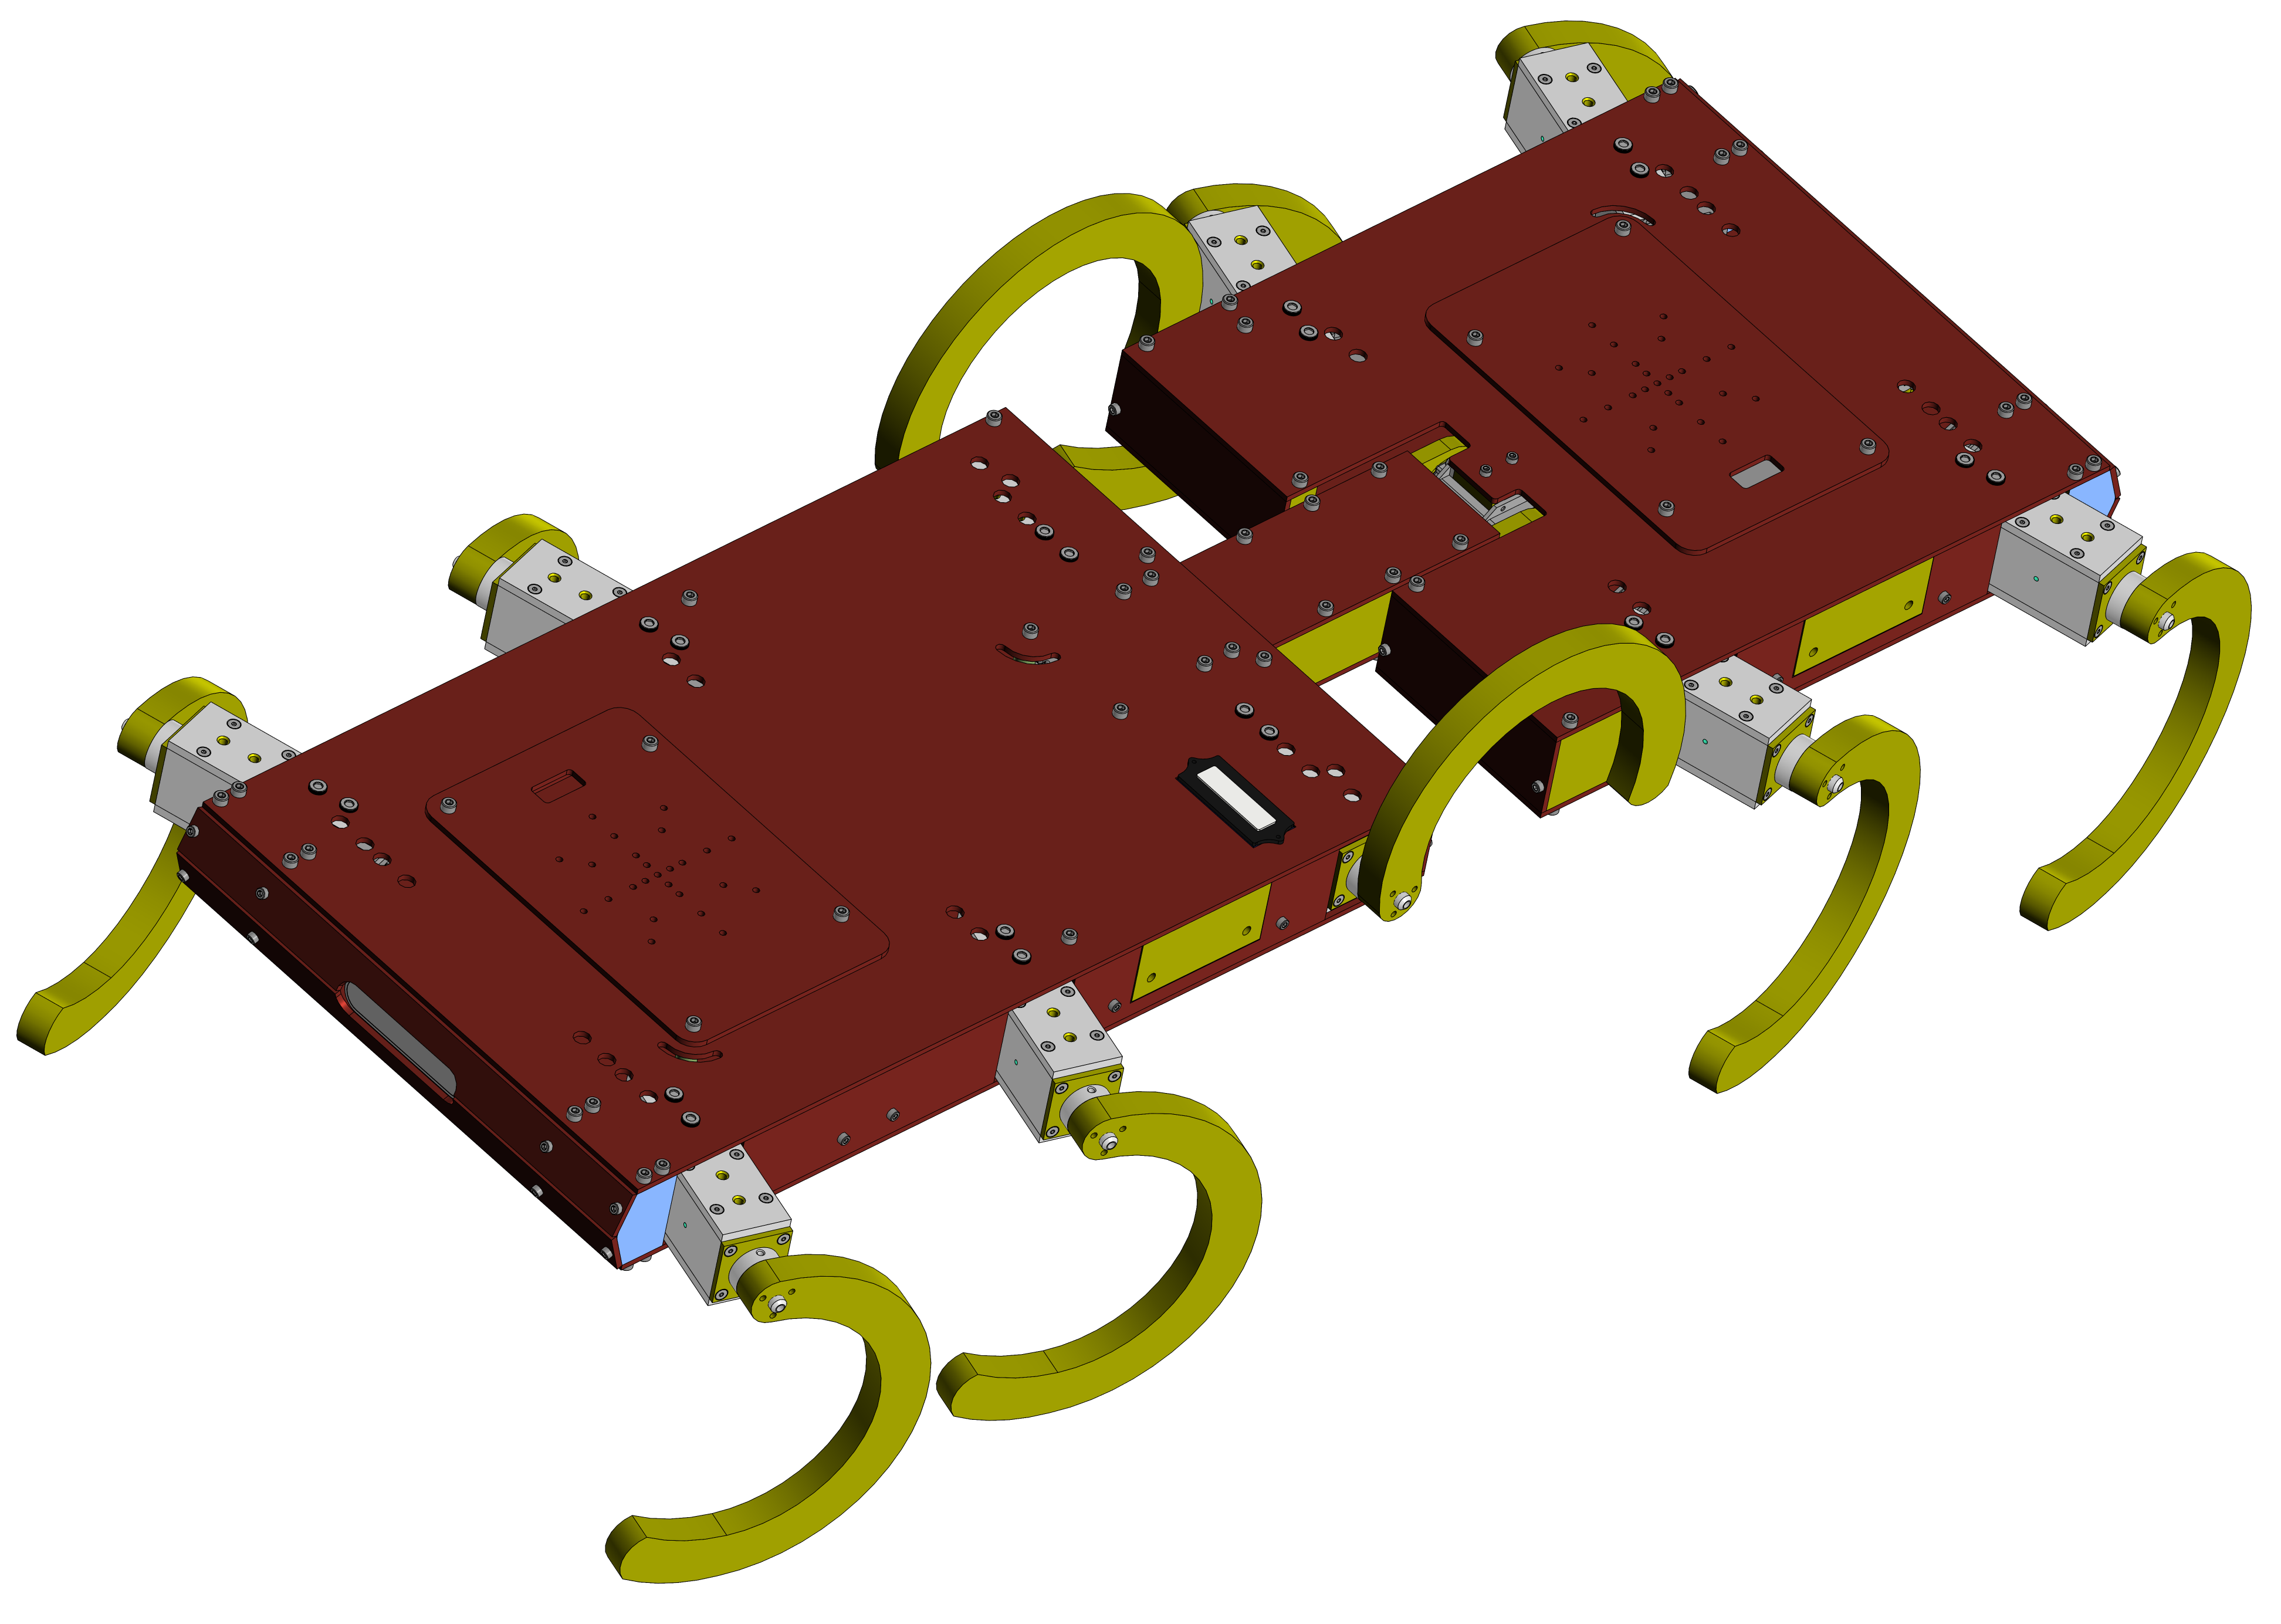
\includegraphics[height=3cm,width=3.5cm,keepaspectratio]{strirus_4.png}} \\
        Поколение & 3+  & 4 \\
         \hline
         \rowcolor[HTML]{EFEFEF} 
         Кол-во ног & 6 & 10 \\ 
         Кол-во сегм. & 1 & 2 \\
         \rowcolor[HTML]{EFEFEF} 
         Соед. узел & --- & Тангаж \\
        \makecell[l]{Отн. угол \\ нога-тело, град} & 0 & 0, 15 \\
        \rowcolor[HTML]{EFEFEF} 
        Высота ноги, мм & 90 & 180 \\
        Особенности & Удлиненные ноги & Гигантские ноги \\
        \rowcolor[HTML]{EFEFEF} 
        Недостатки &  \makecell[l]{-- 1 Сегмент} & \makecell[l]{ -- } \\
        \end{tabular}
        \end{tiny}
        \end{table}
\end{frame}

\begin{frame}[t]{Разработка преобразователя силы}
    \framesubtitle{}
    \only<1-2>{\large\begin{block}{Question}
            Как получить силу реакции опоры?
        \end{block}}
    \only<2>{\large\begin{alertblock}{Answer}
        \vspace{-0.2cm}

         \begin{itemize}
            \color{lightgray}
            \item Измерив ток/напряжение на моторе
                \item Установив датчик момента на вал мотора
                \item {\color{black} Установив датчик силы на ногу робота}
            \end{itemize}
        \end{alertblock}}
\end{frame}

\begin{frame}[t]{Разработка преобразователя силы}
    \framesubtitle{Типы датчиков силы}
    \vspace{-20pt}
    \begin{multicols}{2}
        \begin{itemize}
            \alt<1>{}{\color{lightgray}}
            \item  \textbf{Силомоментный}: массивный и дорогой для маленьких роботов
            \item \textbf{Оптический}: очень габаритный
            \item \textbf{Магнитный}: очень габаритный
            \item \textbf{Емкостной}: дорогой, но лучший для данной задачи
            \item {\color{black}\textbf{Пьезорезистивный датчик основанный \alt<1>{на чернилах или полимерах}{\underline{Velostat}}}: дешевый и надежный, но имеет проблемы с гистерезисом}

            \item { \alt<1>{}{\color{lightgray}} \textbf{Тензометрический}: влияние температуры и влажности на чувствительность}
        \end{itemize}
    \end{multicols}
    \vspace{-10pt}
    \only<2>{\ }
\end{frame}

\begin{frame}[t]{Разработка преобразователя силы}
    \framesubtitle{Velostat}
    \vspace{-20pt}
    \begin{columns}[T,onlytextwidth]
        \begin{column}{0.6\textwidth}
            \begin{exampleblock}{Определение}
                Velostat представляет собой полимерный материал, наполненный техническим углеродом.\\
                \textbf{Ожидаемые эффекты}:
                \begin{itemize}
                    \item \underline{Туннельный эффект} -- диод обладает данным свойством
                    \item \underline{Пьезорезистивный} -- удельное электрическое сопротивление полупроводника изменяется под действием механической деформации
                    \item \underline{Вязкоупругий} -- может гасить вибрации
                \end{itemize}
            \end{exampleblock}
        \end{column}
        \begin{column}{0.38\textwidth}
            \vspace{-1cm}
            \begin{figure}[H]
                \begin{subfigure}{0.9\textwidth}
                    \centering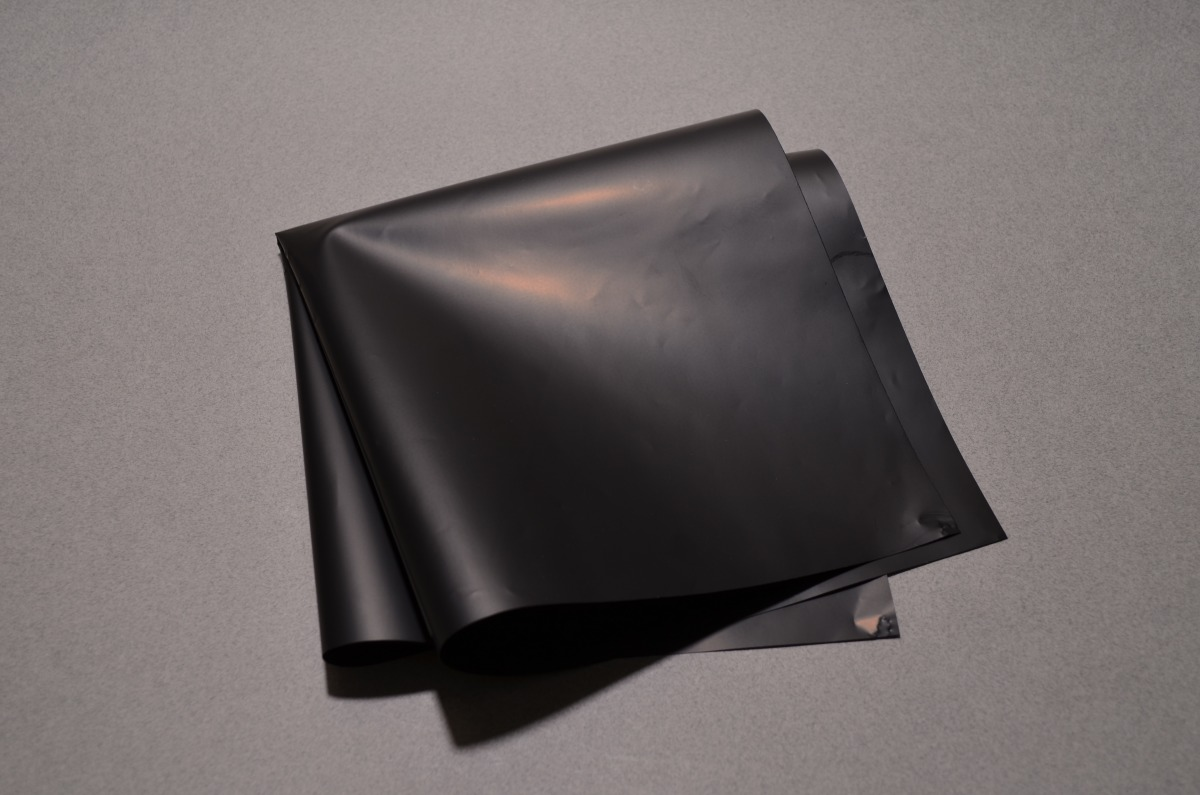
\includegraphics[height=3cm,width=1\textwidth,keepaspectratio]{velostat_sensor.jpg}
                    % \caption*{Velostat material}
                    \label{fig:velostat_sensor.jpg}
                \end{subfigure}

                \begin{subfigure}{0.9\textwidth}
                    \centering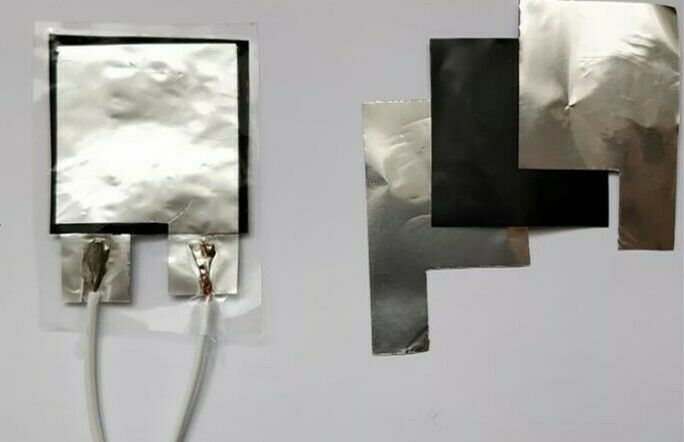
\includegraphics[height=3cm,width=1\textwidth,keepaspectratio]{simplest_sensor.jpg}
                    \caption*{Простейший преобразователь силы}
                    \label{fig:simplest_sensor.jpg}
                \end{subfigure}
            \end{figure}
        \end{column}
    \end{columns}

\end{frame}

\begin{frame}[t]{Разработка преобразователя силы}
    \framesubtitle{Velostat: Встреченные проблемы}
    \vspace{-20pt}
    \begin{multicols}{2}
        {\large
            \begin{itemize}
                \item Гистерезис
                \item Нелинейность материала
                \item Разные значения при одинаковом давлении, если площадь нагрузки меньше площади датчика
            \end{itemize}}
            \begin{figure}[H]
                \centering
                 \begin{tikzpicture}
                    % Include the image in a node
                    \node [above right, inner sep=0] (image) at (0,0) 
                    {\centering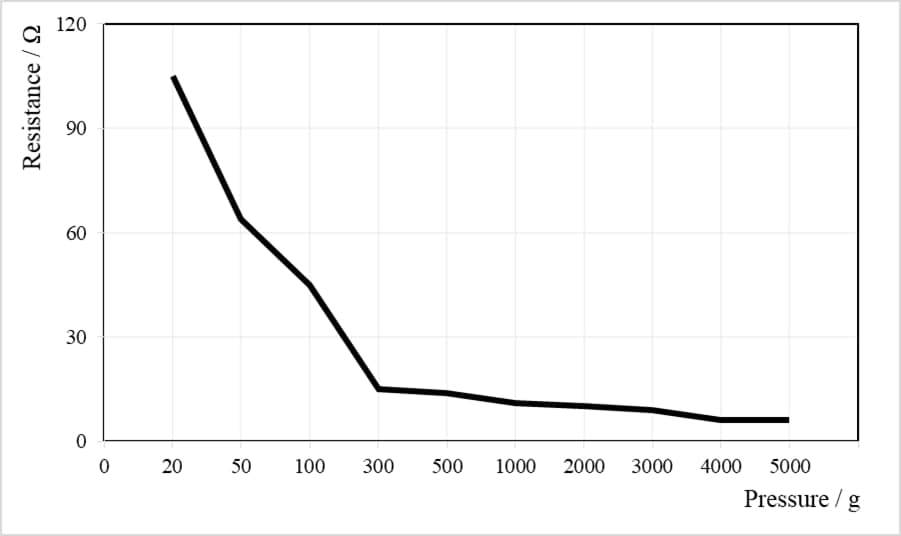
\includegraphics[height=4cm,width=1\textwidth,keepaspectratio]{velostat_pressure_resistance.jpg}};          
                    % Create scope with normalized axes
                    \begin{scope}[
                        x={($ 0.1*(image.south east)$)},
                        y={($ 0.1*(image.north west)$)}]
                        % Grid and axes' labels
                        % \draw[lightgray,step=1] (image.south west) grid (image.north east);
                        % \foreach \x in {0,1,...,10} { \node [below] at (\x,0) {\x}; }
                        % \foreach \y in {0,1,...,10} { \node [left] at (0,\y) {\y};}
             
                        % Labels
                        % \draw[latex-, very thick,green] (3.5,2.2) -- (2.5,1)
                        % node[below left,black,fill=white]{\small test};

                        \draw[stealth-, very thick,green] (4.21,2.75) -- (6.5,5);
                        \draw[stealth-, very thick,green] (8.75,2.15) -- (6.5,5)
                        node[rounded corners=3pt,above,black,fill=white]{\small Working range};
                    \end{scope}
                \end{tikzpicture}
                % \caption*{}
                \label{fig:velostat_pressure_resistance.jpg}
            \end{figure}
    \end{multicols}
    \vspace{-12pt}
    \begin{block}{Научная постановка задачи}
        Охарактеризовать материал Velostat для случаев, когда точечная нагрузка меньше размера датчика, и предложить решения для предотвращения подобных проблем.
    \end{block}
\end{frame}

\begin{frame}[t]{Разработка преобразователя силы}
    \framesubtitle{Требования к установке}
    \vspace{-0.5cm}
    {\large
        \begin{itemize}
            \item Управление силой нажатия \uncover<2>{\\ \alert{Решено с помощью импедансного управления}}
            \item Повторяемость эксперимента по силе и позиции \uncover<2>{\\ \alert{Решено, добавив манипулятор и камеру}}
            \item Возможность нажимать только на часть сенсора \uncover<2>{\\ \alert{Возможно благодаря насадкам для манипулятора}}
        \end{itemize}}
    \uncover<2>{\centering\large\alert{Все требования выполнены}}
\end{frame}


\begin{frame}[t]{Разработка преобразователя силы}
    \framesubtitle{Установка: Общий вид}
    \vspace{-12pt}
    \begin{center}
        \begin{tikzpicture}

            % Include the image in a node
            \node [
                above right,
                inner sep=0] (image) at (0,0) {\centering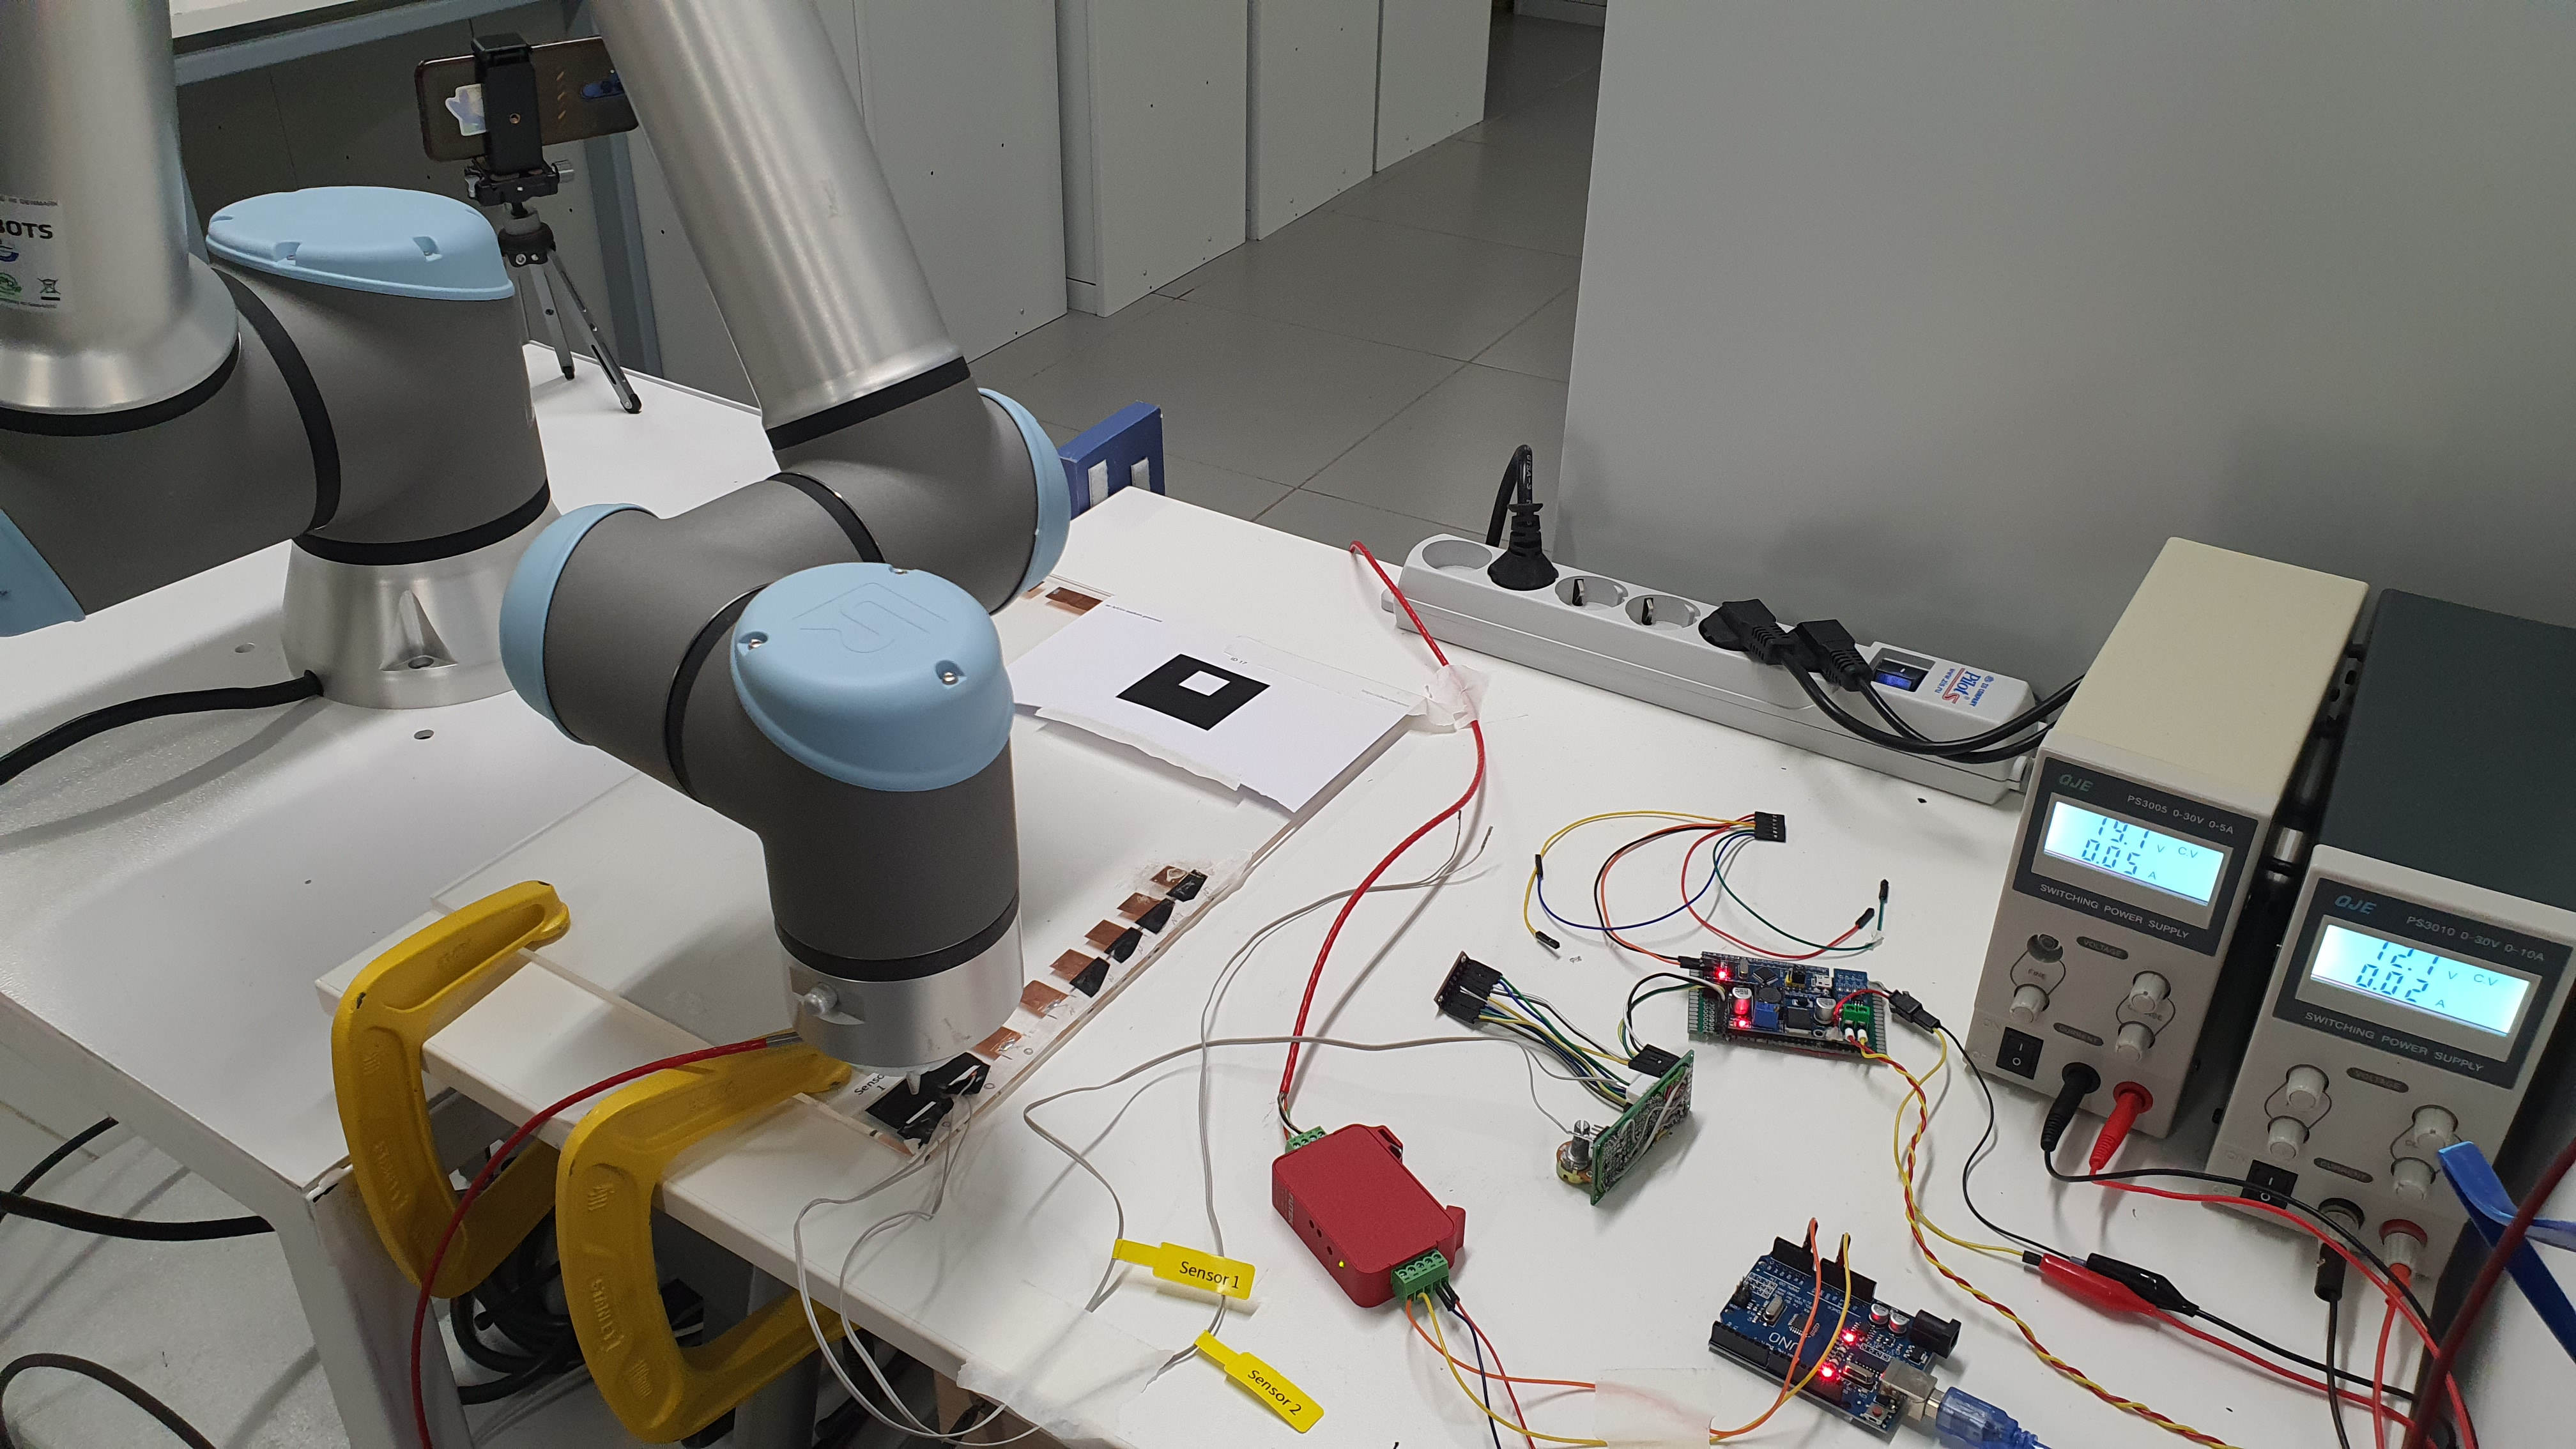
\includegraphics[height=6cm,width=1\textwidth,keepaspectratio]{exp_stand1}};

            % Create scope with normalized axes
            \begin{scope}[
                    x={($0.1*(image.south east)$)},
                    y={($0.1*(image.north west)$)}]

                % Grid
                % \draw[lightgray,step=1] (image.south west) grid (image.north east);

                % % Axes' labels
                % \foreach \x in {0,1,...,10} { \node [below] at (\x,0) {\x}; }
                % \foreach \y in {0,1,...,10} { \node [left] at (0,\y) {\y};}

                % Labels
                % \node[circle,fill=green] at (7.25,6.75){\small 2};

                \draw[latex-, very thick,green] (3.5,2.2) -- (2.5,1)
                node[rounded corners=3pt,below left,black,fill=white]{\small Velostat sensors};

                \draw[stealth-, very thick,green] (3.5,2.6) -- ++(-0.7,+0.5)
                node[rounded corners=3pt,left,black,fill=white]{\small Force sensor};

                \draw[stealth-, very thick,green] (6.5,3) -- (7,6)
                node[rounded corners=3pt,above right,black,fill=white]{\small Self-made PCB};

                \draw[stealth-, very thick,green] (7.2,1.5) -- (8,5)
                node[rounded corners=3pt,above right,black,fill=white]{\small Arduino};

                \draw[stealth-, very thick,green] (2.5,9.5) -- (4,9.5)
                node[rounded corners=3pt,right,black,fill=white]{\small Camera};

                \draw[very thick,green] (0.5,2.5) rectangle (4.2,9)
                node[below left,black,fill=green]{\small UR10e};

                \draw[latex-, very thick,green] (4.5,7.2) edge (5.5,7.5)
                (4.8,5.3) -- (5.5,7.5)
                node[rounded corners=3pt,above,black,fill=white]{\small Aruco markers};
            \end{scope}

        \end{tikzpicture}
    \end{center}
\end{frame}

\begin{frame}[t]{Разработка преобразователя силы}
    \framesubtitle{Установка: Видео}
    \vspace{-15pt}
    \begin{figure}[H]
        % \href{run:./videos/exp_stand_video.mp4}{
        \href{https://youtu.be/Gw4wVZ-ESuE}{
            \centering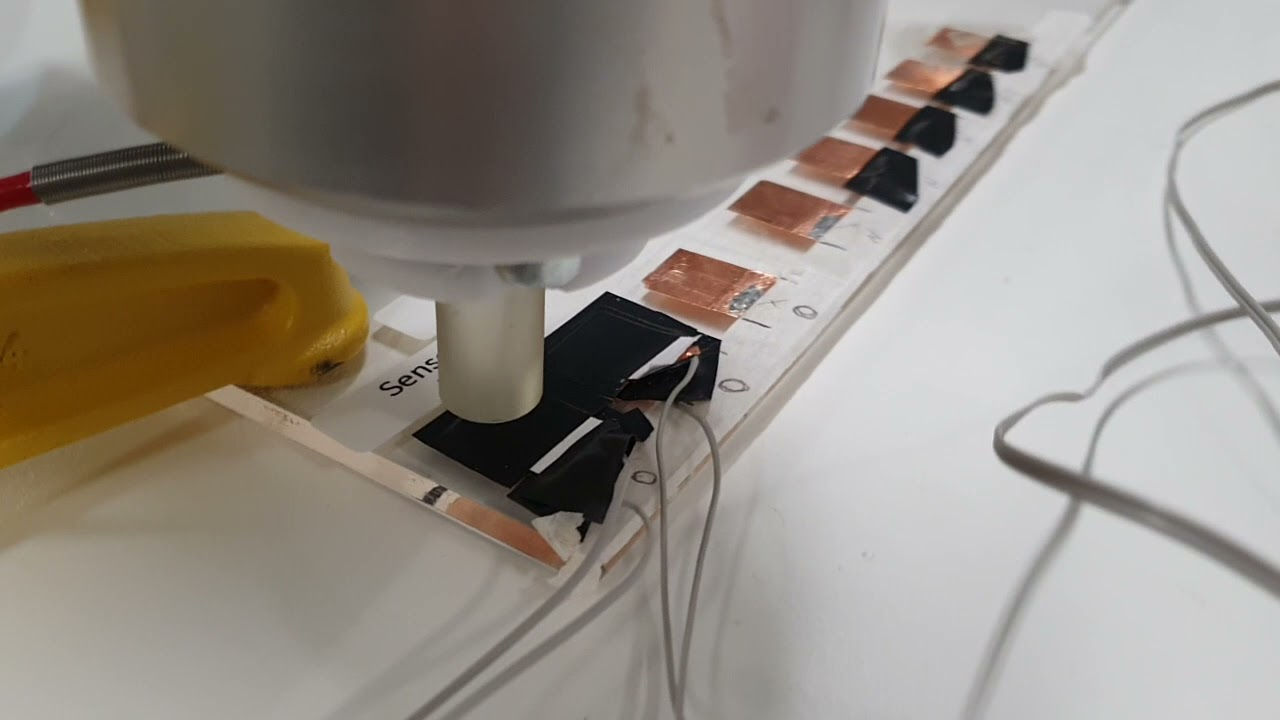
\includegraphics[height=6cm,width=1\textwidth,keepaspectratio]{exp_stand_video_preview.jpg}}
        % \caption{caption_name}
    \end{figure}
\end{frame}

\begin{frame}[t]{Разработка преобразователя силы}
    \framesubtitle{Установка: Снижение ошибки по углу с помощью Aruco маркеров}
    \vspace{-15pt}

    \begin{figure}[H]
        \centering
         \begin{tikzpicture}
            % Include the image in a node
            \node [above right, inner sep=0] (image) at (0,0) 
            {\centering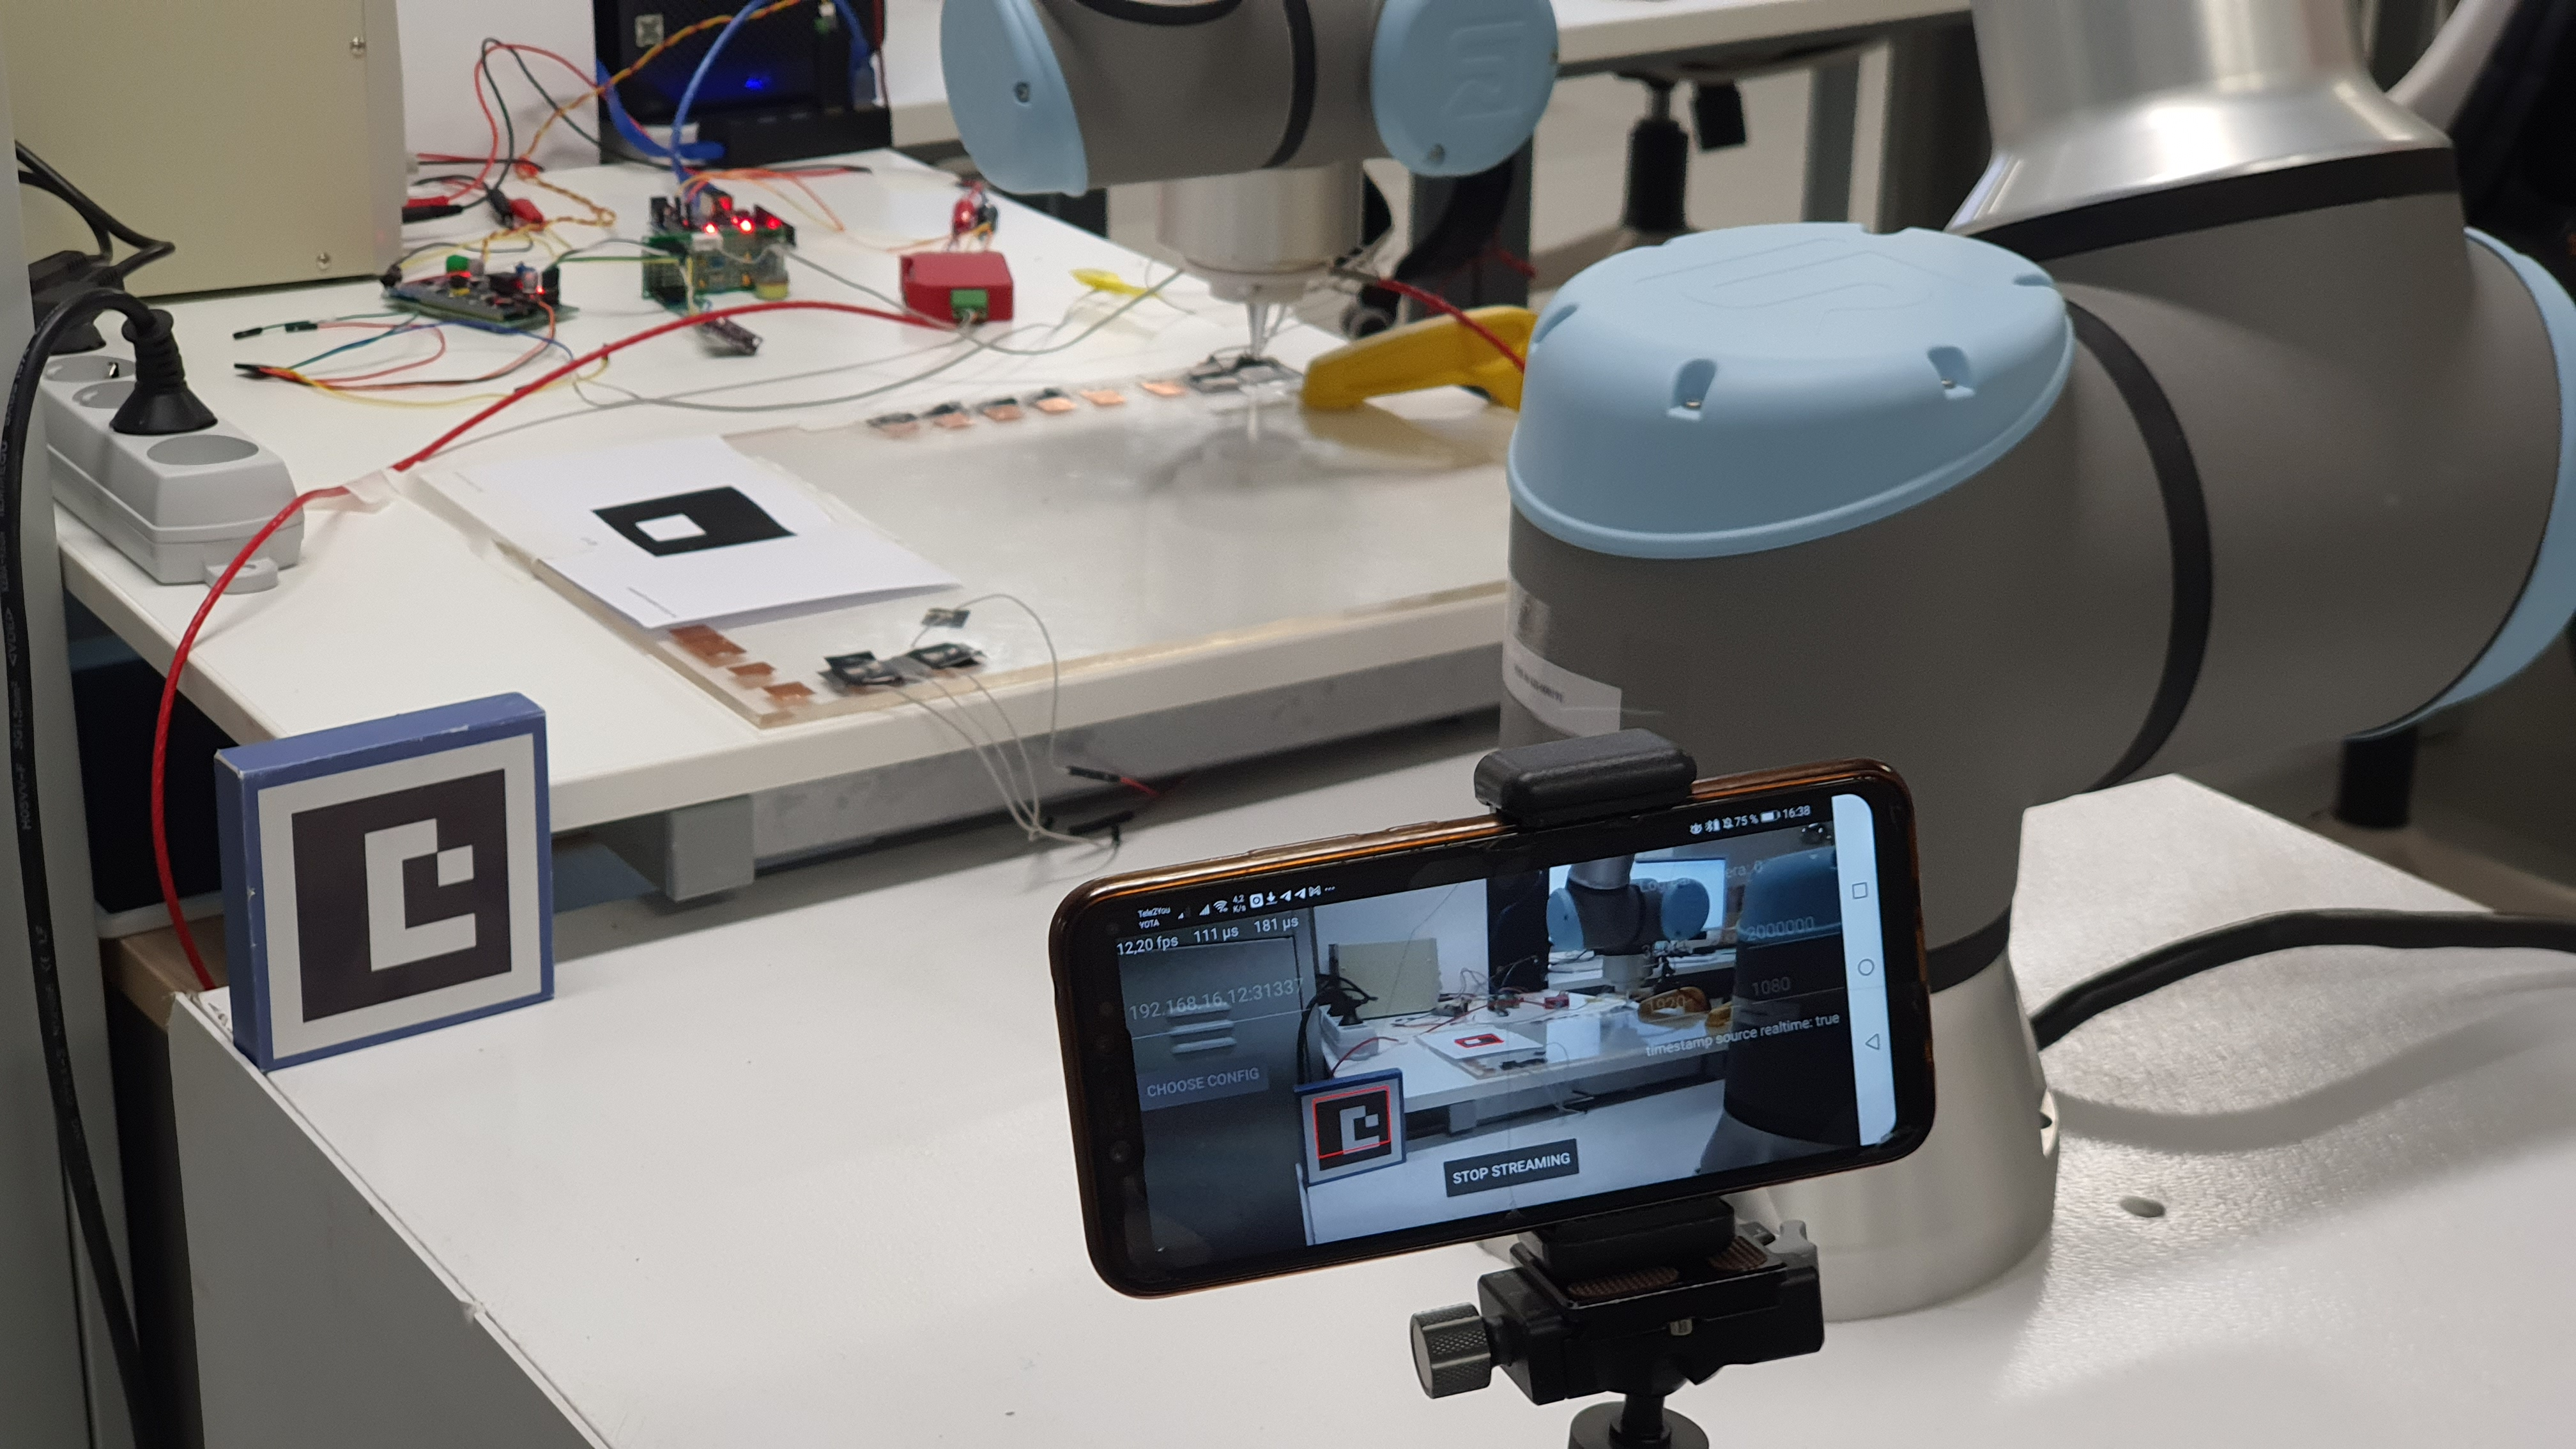
\includegraphics[height=6cm,width=1\textwidth,keepaspectratio]{exp_stand2.JPG}};          
            % Create scope with normalized axes
            \begin{scope}[
                x={($ 0.1*(image.south east)$)},
                y={($ 0.1*(image.north west)$)}]
                % Grid and axes' labels
                % \draw[lightgray,step=0.5] (image.south west) grid (image.north east);
                % \foreach \x in {0,1,...,10} { \node [below] at (\x,0) {\x}; }
                % \foreach \y in {0,1,...,10} { \node [left] at (0,\y) {\y};}
                % Labels
                \draw[stealth-, very thick,green] (1.2,3) -- (1.2,2)
                node[rounded corners=3pt,below,black,fill=white, text width=2cm]{\small Manip. base Aruco marker};  

                \draw[stealth-, very thick,green] (2.3,6.5) -- (1.5,7.5)
                node[rounded corners=3pt,above,black,fill=white, text width=2cm]{\small Sensor plate Aruco marker};  

                \draw[stealth-, very thick,green] (5.4,2) -- (7.5,1.5);
                \draw[stealth-, very thick,green] (5.75,2.8) -- (7.5,1.5)
                node[rounded corners=3pt,right,black,fill=white, text width=2.3cm]{\small Transformation calculation b/w markers};  
            \end{scope}
        \end{tikzpicture}
        % \caption*{}
        \label{fig:exp_stand2.JPG}
    \end{figure}

\end{frame}

\begin{frame}[t]{Разработка преобразователя силы}
    \framesubtitle{Установка: Насадки}
    \vspace{-0.9cm}
    \begin{columns}[T,onlytextwidth]
        \begin{column}{0.6\textwidth}
            \begin{figure}[H]
                \centering
                \begin{tikzpicture}
                    % Include the image in a node
                    \node [above right, inner sep=0] (image) at (0,0)
                    {\centering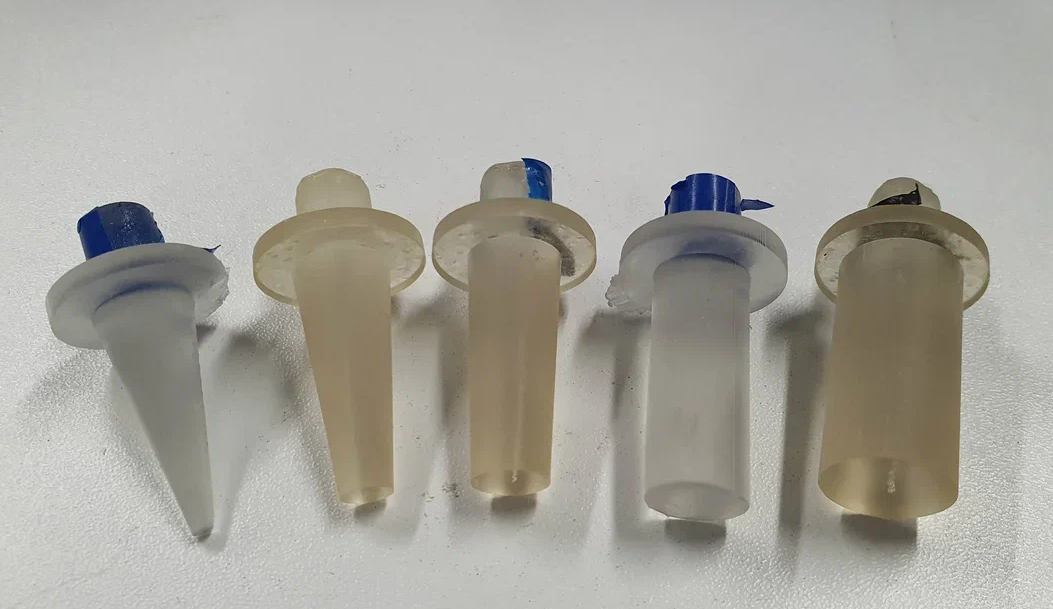
\includegraphics[height=5cm,width=1\textwidth,keepaspectratio]{all_end_effectors.png}};
                    % Create scope with normalized axes
                    \begin{scope}[
                            x={($ 0.1*(image.south east)$)},
                            y={($ 0.1*(image.north west)$)}]
                        % Grid and axes' labels
                        % \draw[lightgray,step=1] (image.south west) grid (image.north east);
                        % \foreach \x in {0,1,...,10} { \node [below] at (\x,0) {\x}; }
                        % \foreach \y in {0,1,...,10} { \node [left] at (0,\y) {\y};}

                        % Labels
                        \node[rounded corners=3pt,black,fill=white] at (1.1,7.4){\tiny 2 mm };
                        \node[rounded corners=3pt,black,fill=white] at (3.1,7.9){\tiny 6 mm };
                        \node[rounded corners=3pt,black,fill=white] at (4.9,8.1){\tiny 8 mm };
                        \node[rounded corners=3pt,black,fill=white] at (6.7,7.9){\tiny 12 mm };
                        \node[rounded corners=3pt,black,fill=white] at (8.6,7.9){\tiny 15 mm };
                    \end{scope}
                \end{tikzpicture}
                \caption*{Все насадки}
                \label{fig:all_end_effectors.png}
            \end{figure}
        \end{column}
        \begin{column}{0.39\textwidth}
            \vspace{-1.3cm}

            \begin{figure}[H]
                \begin{subfigure}[t]{0.6\textwidth}
                    \centering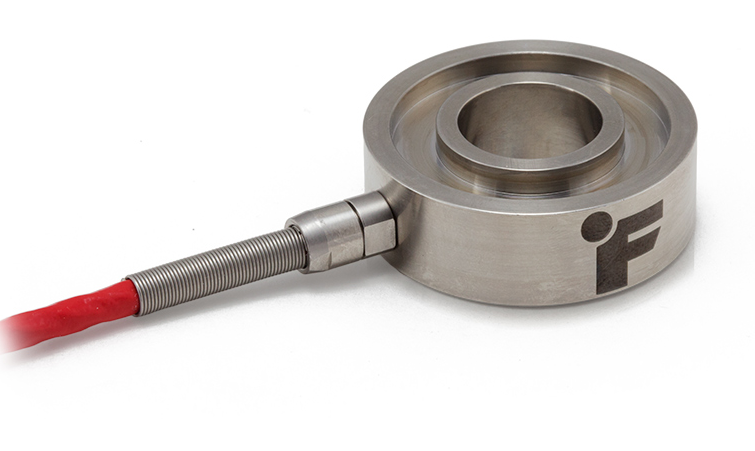
\includegraphics[width=0.99\textwidth]{LTH350-DONUT-LOAD-CELL-1.png}\\
                    \caption*{\normalsize Промышленный \\ датчик силы}
                    \label{fig:futek}
                \end{subfigure}
                \vspace{-0.2cm}

                \begin{subfigure}[t]{0.6\textwidth}
                    \centering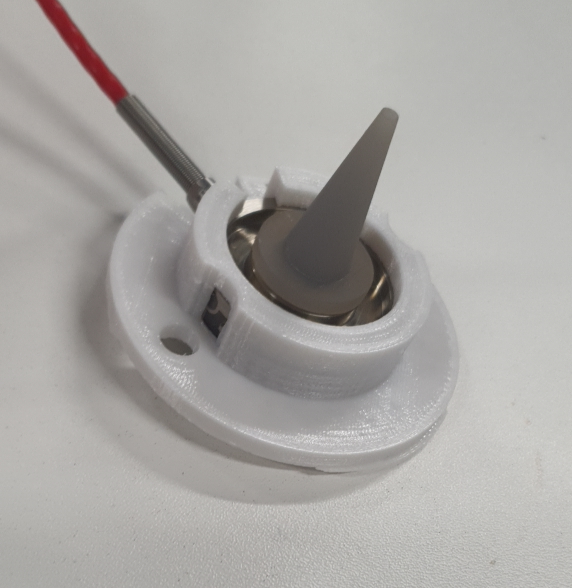
\includegraphics[width=0.99\textwidth]{point_load.JPG}\\
                    \caption*{\normalsize Насадка в сборке}
                    \label{fig:point_load}
                \end{subfigure}
            \end{figure}

        \end{column}
    \end{columns}
\end{frame}




\begin{frame}[t]{Разработка преобразователя силы}
    \framesubtitle{Эксперименты}
    \vspace{-15pt}
    \begin{columns}[T,onlytextwidth]
        \begin{column}{0.6\textwidth}
            {\large
                \begin{enumerate}
                    \item \textbf{Статический}. Прикладывается статический груз с размером в сенсор
                          \item\textbf{Динамический}.
                          \begin{itemize}
                            \large
                              \item Преобразователь представляется в виде сетки $4\times4$. Мы касаемся с одинаковым давлением, используя все 5 насадок
                              \item Используются насадки только 2 и 15 мм. Происходит нажатие с силой 5, 10, 20, 30, 40 H
                          \end{itemize}
                \end{enumerate}
            }
        \end{column}
        \begin{column}{0.39\textwidth}
            \vspace{-0.5cm}
            \begin{figure}[H]
                \centering
                \begin{tikzpicture}

                    % Include the image in a node
                    \node [
                        above right,
                        inner sep=0] (image) at (0,0) {\centering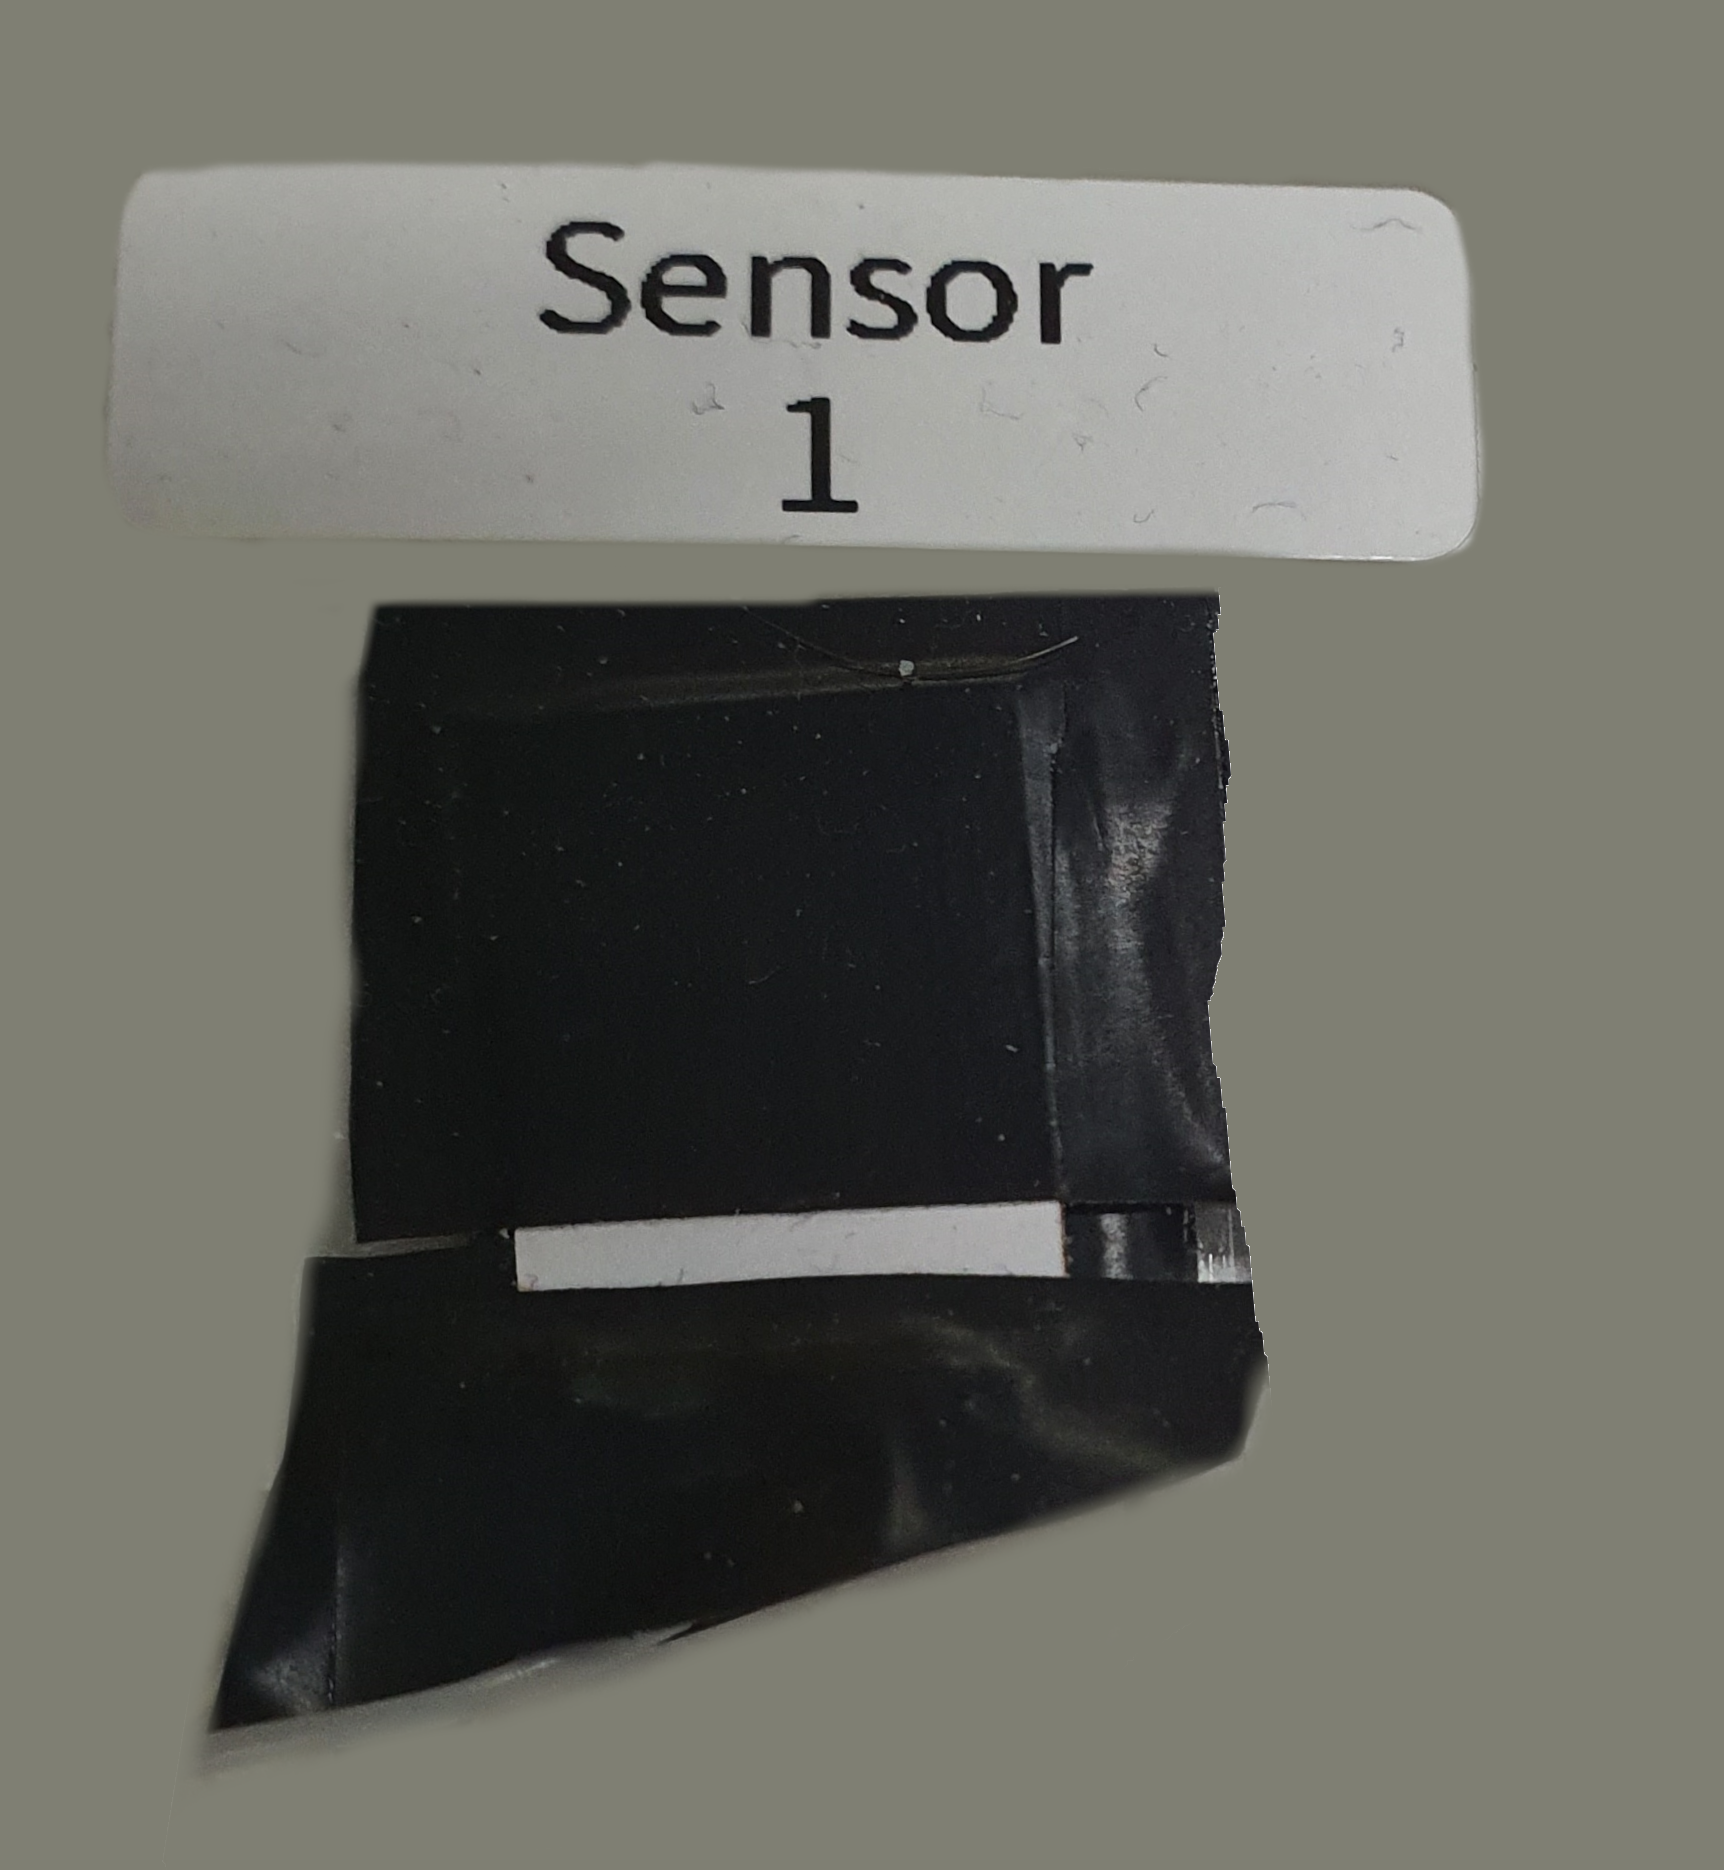
\includegraphics[height=5cm,width=1\textwidth,keepaspectratio]{sensors_grid.png}};

                    % Create scope with normalized axes
                    \begin{scope}[
                            x={($0.1*(image.south east)$)},
                            y={($0.1*(image.north west)$)}]

                        % Grid
                        % \draw[lightgray,step=1] (image.south west) grid (image.north east);

                        % % Axes' labels
                        % \foreach \x in {0,1,...,10} { \node [below] at (\x,0) {\x}; }
                        % \foreach \y in {0,1,...,10} { \node [left] at (0,\y) {\y};}

                        % Labels
                        % Simple brace
                        \draw [green, very thick,
                            decorate,
                            decoration = {brace,
                                    raise=5pt,
                                    amplitude=5pt,
                                    aspect=0.5}] (6,3.7) --  (3,3.7)
                        node[pos=0.5,below=10pt,green]{$15\ mm$};

                        \draw [green, very thick,
                            decorate,
                            decoration = {brace, mirror,
                                    raise=5pt,
                                    amplitude=5pt,
                                    aspect=0.5}] (6,3.6) --  (6,6.4)
                        node[pos=0.5,right=10pt,green]{$15\ mm$};

                        \draw[green,step=1,xshift=34, yshift=43]  (0.5,0.5) grid +(3,3);

                        \node[circle,fill=green,scale=0.4] at (3.3,6.27){\small 1};
                        \node[circle,fill=green,scale=0.4] at (5.92,3.7){\small 16};
                    \end{scope}

                \end{tikzpicture}
                \caption*{Представление сенсора \\ как $4\times4$ сетки}
                \label{fig:file_name}
            \end{figure}
        \end{column}
    \end{columns}
\end{frame}

\begin{frame}[t]{Разработка преобразователя силы}
    \framesubtitle{Результаты: Статический эксперимент}
    \vspace{-0.5cm}
    \begin{columns}[T,onlytextwidth]
        \begin{column}{0.52\textwidth}
            \begin{eqnarray*}
                V_{out} = V_0 + p[k_p + k_e(1-e^\frac{-(t-t_0)}{\tau_{res}})](1-e^{-\frac{A}{p}}) \\
                k_p = A_1e^{-A_2p}; \tau_{res} = B_0 + B_1e^{-\frac{p}{B_2}}
            \end{eqnarray*}
            Где $V_0$ -- начальное напряжение, $p,\ A_i,\ B_i,\ \tau_{res},\ k_i$ константы, $t$ -- текущее время, $t_0$ -- время начала нажатия.
        \end{column}
        \begin{column}{0.45\textwidth}
            \vspace{-15pt}
            \begin{figure}[H]
                \begin{subfigure}{0.99\textwidth}
                    \centering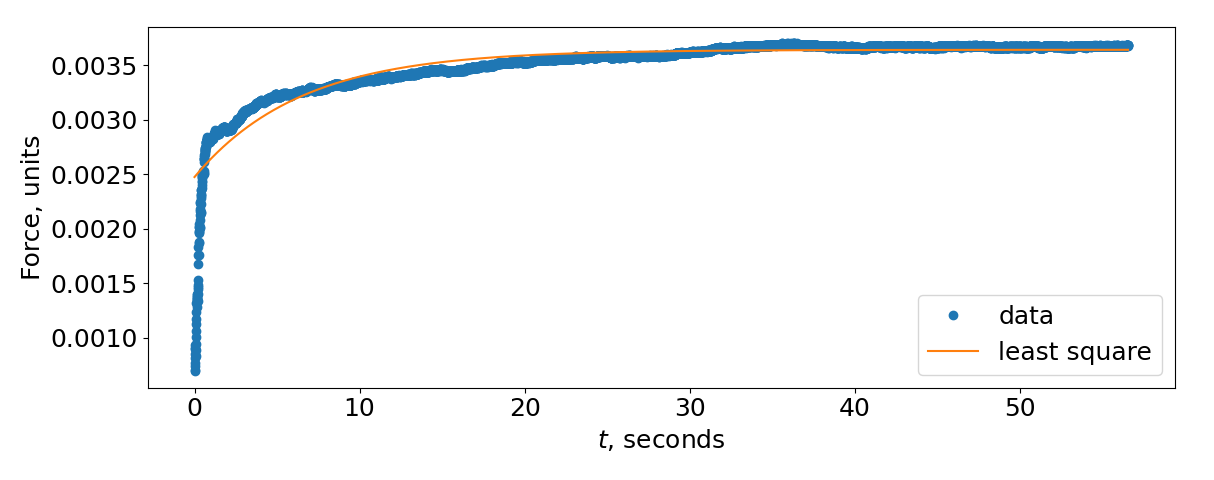
\includegraphics[height=2.8cm,width=1\textwidth,keepaspectratio]{least_square_model.png}
                    \label{fig:least_square_model.png}
                \end{subfigure}
                \vspace{-1cm}

                \begin{subfigure}{0.99\textwidth}
                        \centering
                         \begin{tikzpicture}
                            % Include the image in a node
                            \node [above right, inner sep=0] (image) at (0,0) 
                            {\centering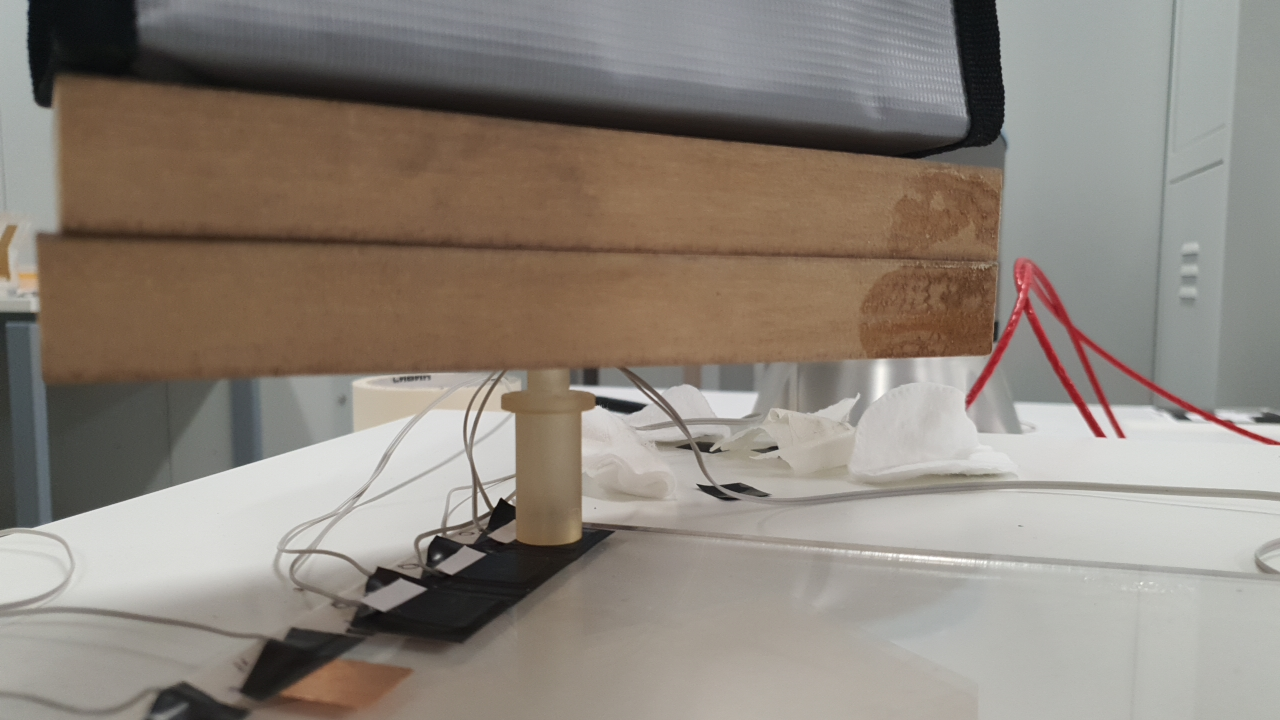
\includegraphics[height=3.4cm,width=1\textwidth,keepaspectratio]{static_load_meh.JPG}};          
                            % Create scope with normalized axes
                            \begin{scope}[
                                x={($ 0.1*(image.south east)$)},
                                y={($ 0.1*(image.north west)$)}]
                                % Grid and axes' labels
                                % \draw[lightgray,step=1] (image.south west) grid (image.north east);
                                % \foreach \x in {0,1,...,10} { \node [below] at (\x,0) {\x}; }
                                % \foreach \y in {0,1,...,10} { \node [left] at (0,\y) {\y};}
                                % Labels
                            \draw[latex-, very thick,green] (4.3,2.3) -- (5,1.6)
                                node[rounded corners=3pt,below right,black,fill=white]{\tiny Velostat sensor};
                            
                            \draw[latex-, very thick,green] (4.3,3.5) -- (5.5,2.45)
                                node[rounded corners=3pt,right,black,fill=white]{\tiny \O \ 15 mm end-effector};

                            \draw[latex-, very thick,green] (6,6) -- (6.4,4.9)
                                node[rounded corners=3pt,below right,black,fill=white]{\tiny Known static load};
                            \end{scope}
                        \end{tikzpicture}
                        % \caption*{}
                \end{subfigure}
            \end{figure}
        \end{column}
    \end{columns}
\end{frame}

\begin{frame}[t]{Разработка преобразователя силы}
    \framesubtitle{Результаты: Динамический эксперимент}
    \vspace{-15pt}
    \begin{figure}[H]
        \begin{subfigure}{0.64\textwidth}
            \centering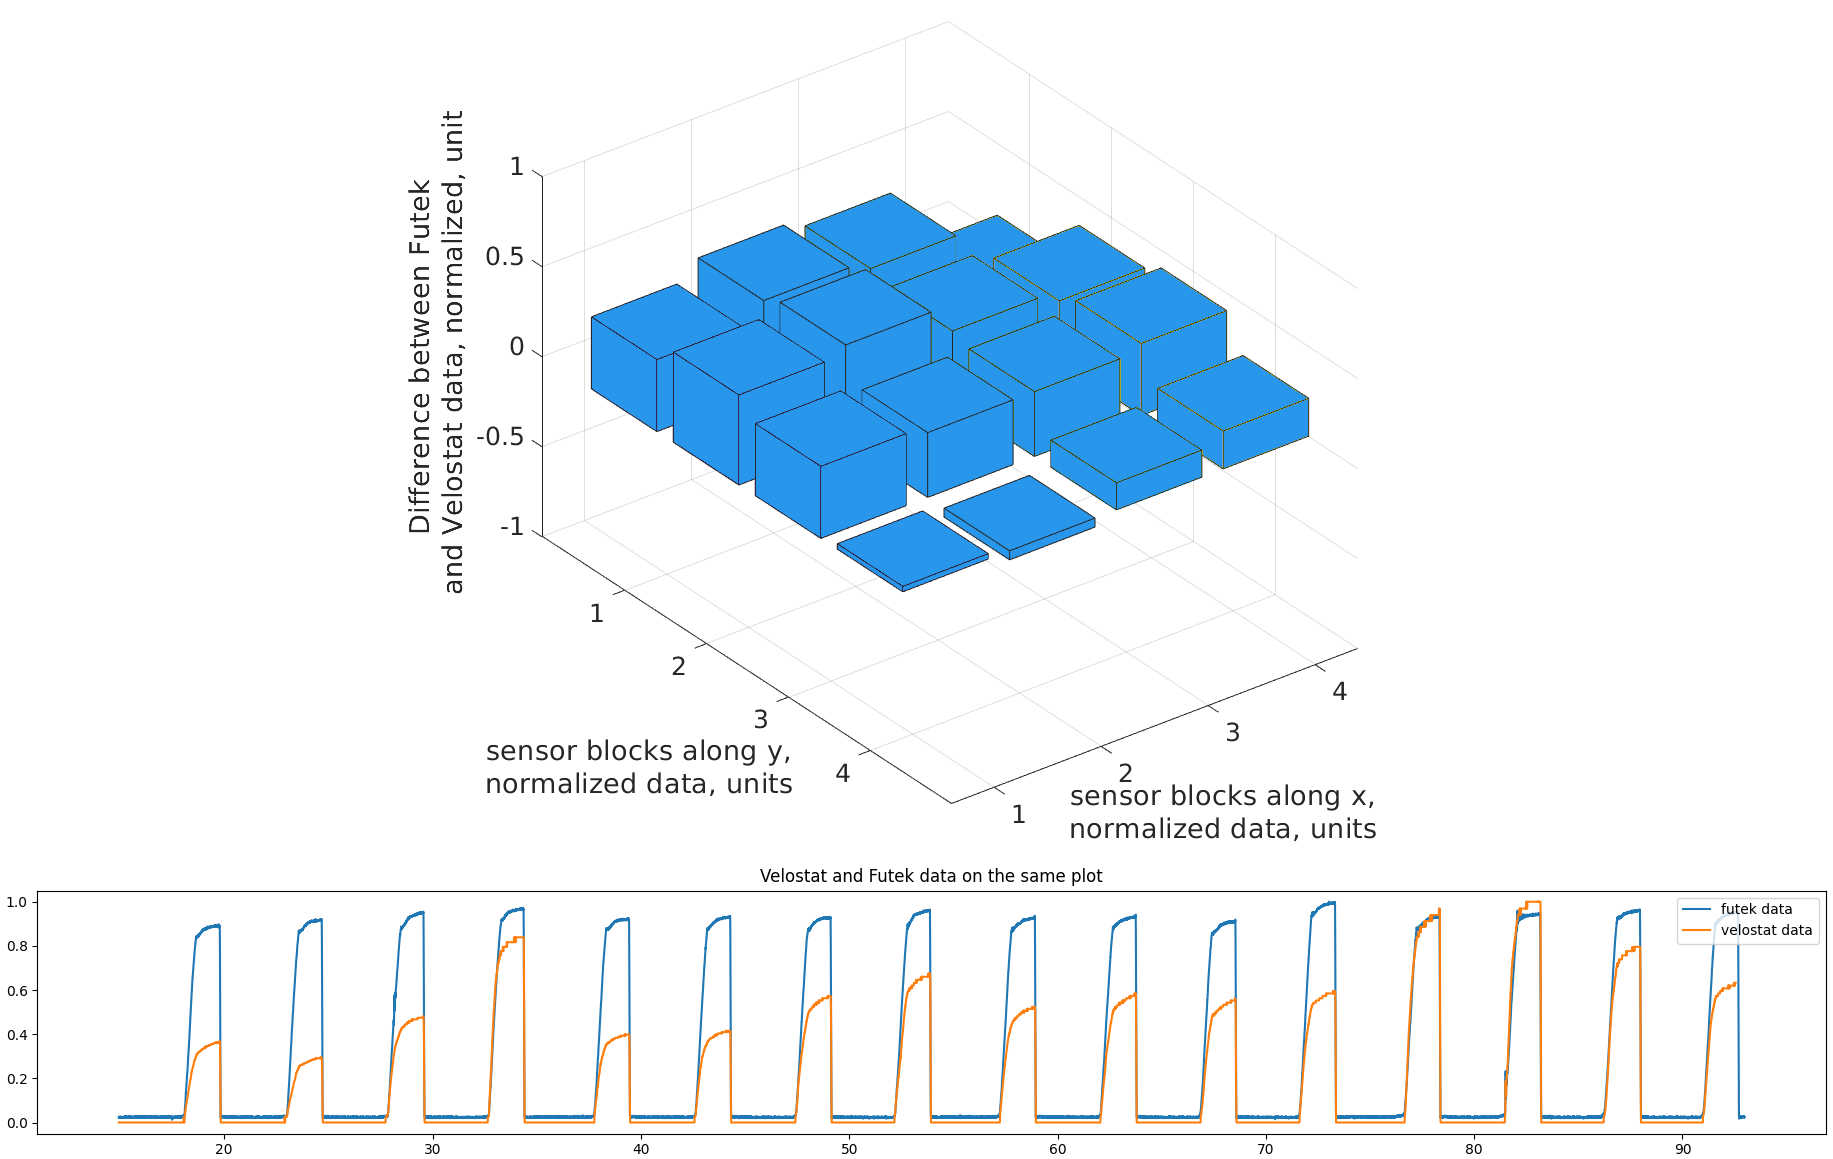
\includegraphics[height=5cm,width=1\textwidth,keepaspectratio]{sens1_pike1_mod.png}
            \caption*{2 мм диаметр насадки}
            \label{fig:sens1_pike1}
        \end{subfigure}
        \begin{subfigure}{0.34\textwidth}
            \centering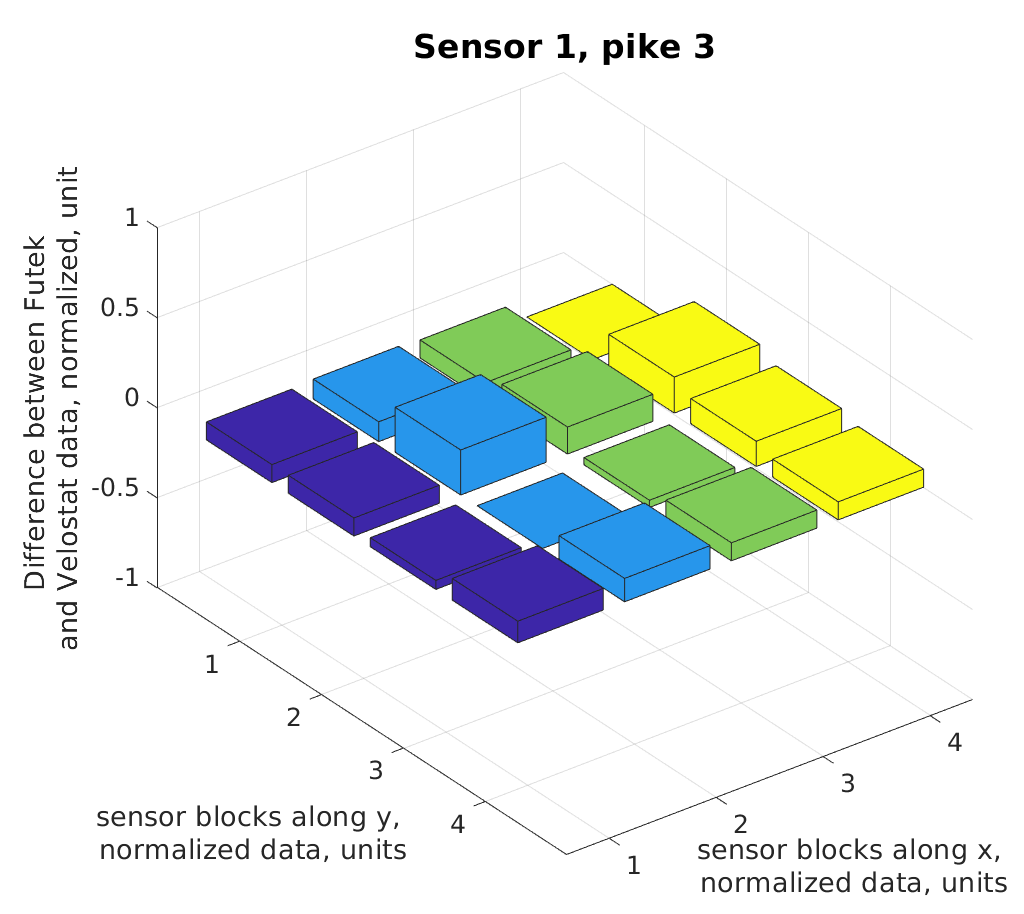
\includegraphics[height=5cm,width=1\textwidth,keepaspectratio]{sens1_pike3.png}
            \caption*{8 мм диаметр насадки}
            \label{fig:sens1_pike3}
        \end{subfigure}
    \end{figure}
\end{frame}

\begin{frame}[t]{Разработка преобразователя силы}
    \framesubtitle{Итог}
    \vspace{-15pt}
    {\large
    \begin{enumerate}
        \item Статический эксперимент: определены коэффициенты преобразователей $p,\ A_i,\ B_i,\ \tau_{res},\ k_i$.
        \item Динамический эксперимент: преобразователь может быть представлен как единое тело, если площадь давления превышает 50\% от площади датчика.
    \end{enumerate}
    }
\end{frame}

\begin{frame}[t]{Определение типа поверхности}
    \framesubtitle{}
    \only<1-2>{\large\begin{block}{Вопрос}
        Как определить тип местности во время движения по такой местности?
        \end{block}}
    \only<2>{\large\begin{alertblock}{Ответ}
            \centering Решенить проблему классификации местности с помощью машинного обучения
        \end{alertblock}}
\end{frame}

\begin{frame}[t]{Определение типа поверхности}
    \framesubtitle{Требования к установке}
    \vspace{-0.5cm}
    {\large
    \begin{itemize}
        \item Иметь возможность быстро менять используемые поверхности \uncover<2>{\\ \alert{Решается с помощью быстроразборного стола}}
        \item Бесконечное движение робота \uncover<2>{\\ \alert{Решается путем создания 2-ух степенного механизма и ноги S-образной формы}}
        \item Узел движителя должен быть такой же как на СтриРусе \uncover<2>{\\ \alert{Решено путем создания крепления для узла ноги}}
    \end{itemize}}
\only<2>{\centering\large\alert{Все требования выполнены}}
\end{frame}

\begin{frame}[t]{Определение типа поверхности}
    \framesubtitle{Установка}
    \vspace{-15pt}
    \begin{columns}[T,onlytextwidth]
        \begin{column}{0.55\textwidth}
            % \begin{enumerate}
            %     \item Dynamixel MX28 -- 47 rev/min
            %     \item Velostat transducer -- 25 HZ freq.
            %     \item Experiment duration -- 120 sec
            % \end{enumerate}
            \vspace{-0.3cm}
            \begin{figure}[H]
                \centering
                \begin{tikzpicture}
                    % Include the image in a node
                    \node [above right, inner sep=0] (image) at (0,0)
                    {\centering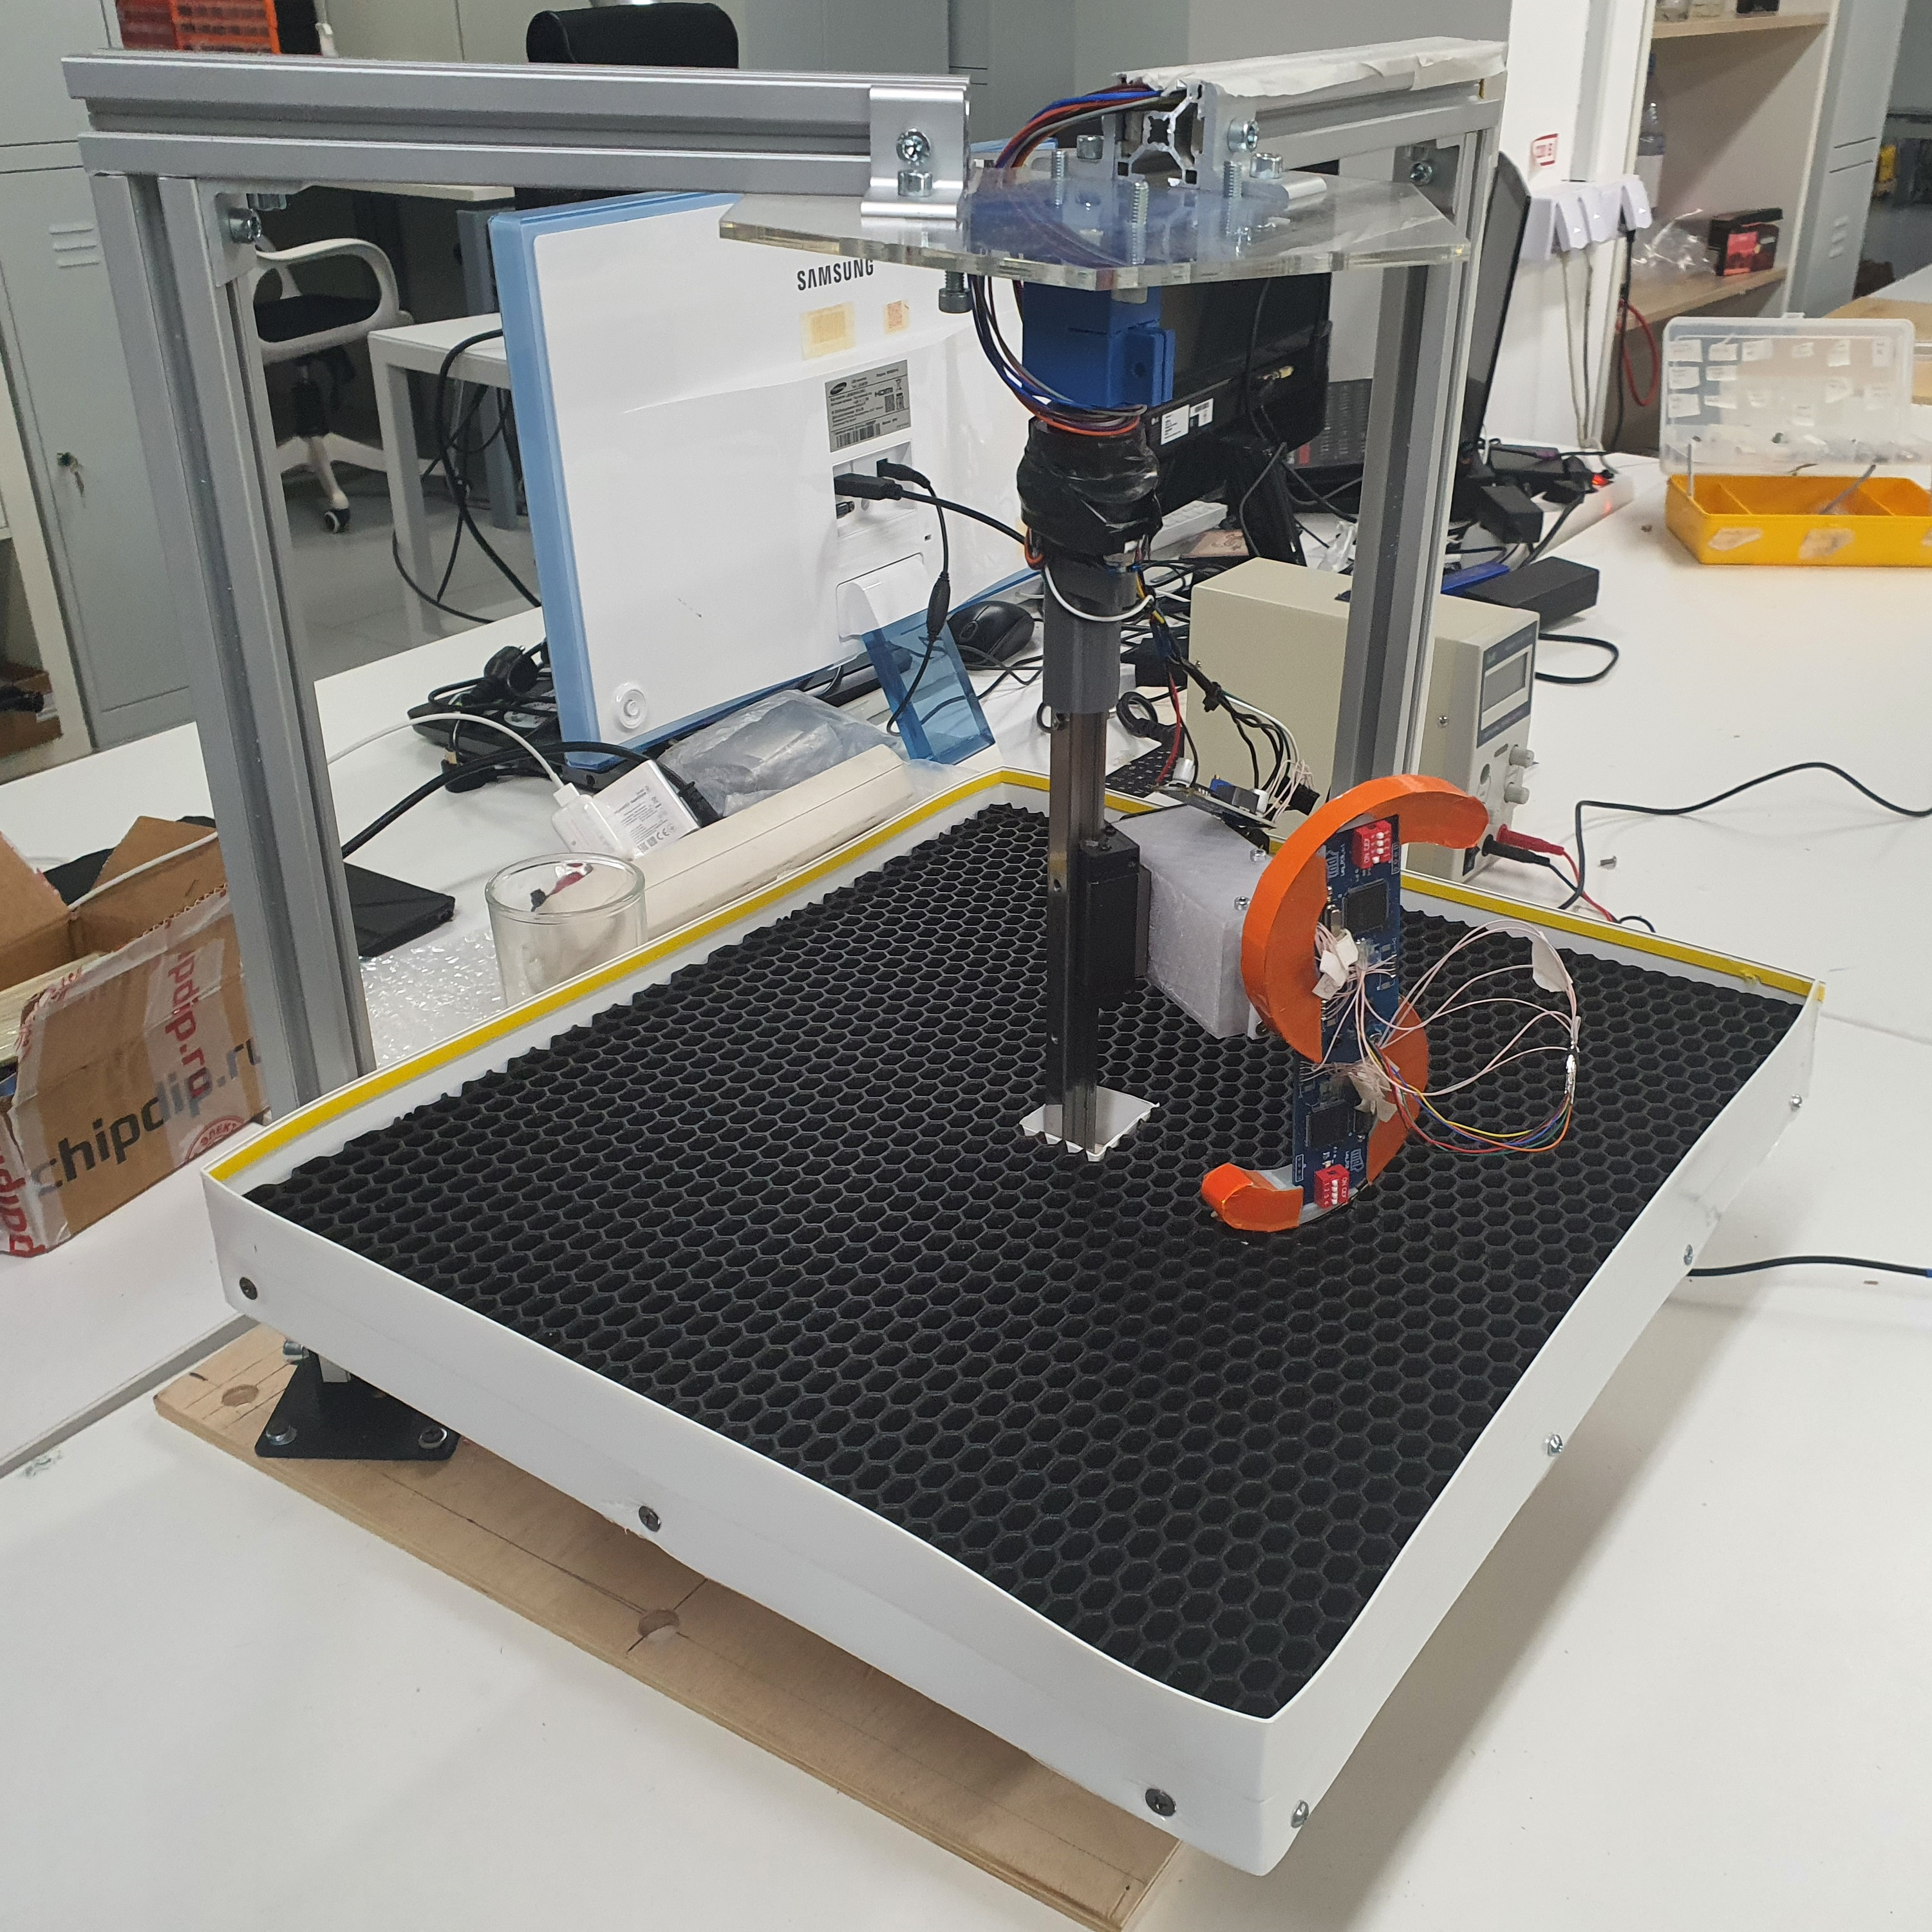
\includegraphics[height=6cm,width=1\textwidth,keepaspectratio]{s_shape_leg/s_leg_setup.JPG}};
                    % Create scope with normalized axes
                    \begin{scope}[
                            x={($ 0.1*(image.south east)$)},
                            y={($ 0.1*(image.north west)$)}]
                        % Grid and axes' labels
                        % \draw[lightgray,step=1] (image.south west) grid (image.north east);
                        % \foreach \x in {0,1,...,10} { \node [below] at (\x,0) {\x}; }
                        % \foreach \y in {0,1,...,10} { \node [left] at (0,\y) {\y};}

                        % Labels

                        % \node[circle,fill=green,scale=0.4] at (3.3,6.27){\small 1};

                        % \draw[latex-, very thick,green] (3.5,2.2) -- (2.5,1)
                        % node[below left,black,fill=white]{\small test};

                        \draw[stealth-, very thick,green] (3.5,2.5) -- (3,1.5)
                        node[rounded corners=3pt,below,black,fill=white]{\tiny Table for surfaces};

                        \draw[stealth-, very thick,green] (7.1,5.4) -- (7.4,7)
                        node[rounded corners=3pt,above right,black,fill=white]{\tiny Self-made PCB};

                        \draw[very thick,green] (6,6.1) rectangle (8.5,3.5)
                        node[above left,black,fill=green]{\tiny S leg};
                    \end{scope}
                \end{tikzpicture}
                % \caption*{}
                \label{fig:s_shape_leg/s_leg_setup.JPG}
            \end{figure}
        \end{column}
        \begin{column}{0.44\textwidth}
            \vspace{-0.5cm}
            \begin{figure}[H]
                \begin{subfigure}{\textwidth}
                    \centering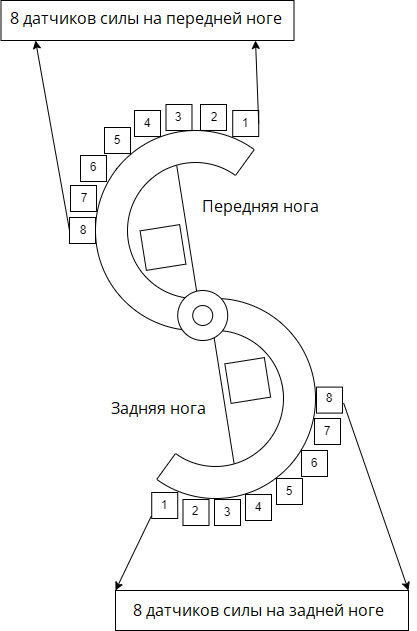
\includegraphics[height=6cm,width=1\textwidth,keepaspectratio]{s_shape_leg/leg_design.png}
                    % \caption{caption_name}
                \end{subfigure}
            \end{figure}
        \end{column}
    \end{columns}
\end{frame}


\begin{frame}[t]{Определение типа поверхности}
    \framesubtitle{Установка: Типы поверхности, видео}
    \vspace{-15pt}
    \begin{figure}[H]
        \begin{subfigure}{0.49\textwidth}
            % \href{run:./videos/flat.gif}
            \href{https://gifyu.com/image/SxatY}
            {\centering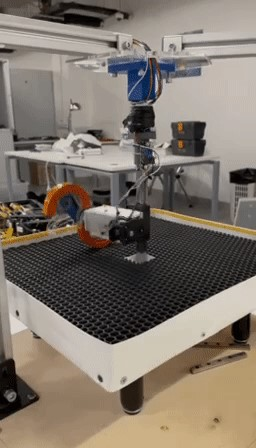
\includegraphics[height=6cm,width=1\textwidth,keepaspectratio]{s_shape_leg/flat.jpg}}
            % \caption*{2mm end-effector diam}    
        \end{subfigure}
        \hfill
        \begin{subfigure}{0.49\textwidth}
            % \href{run:./videos/rock.gif}
            \href{https://gifyu.com/image/Sxatt}
            {\centering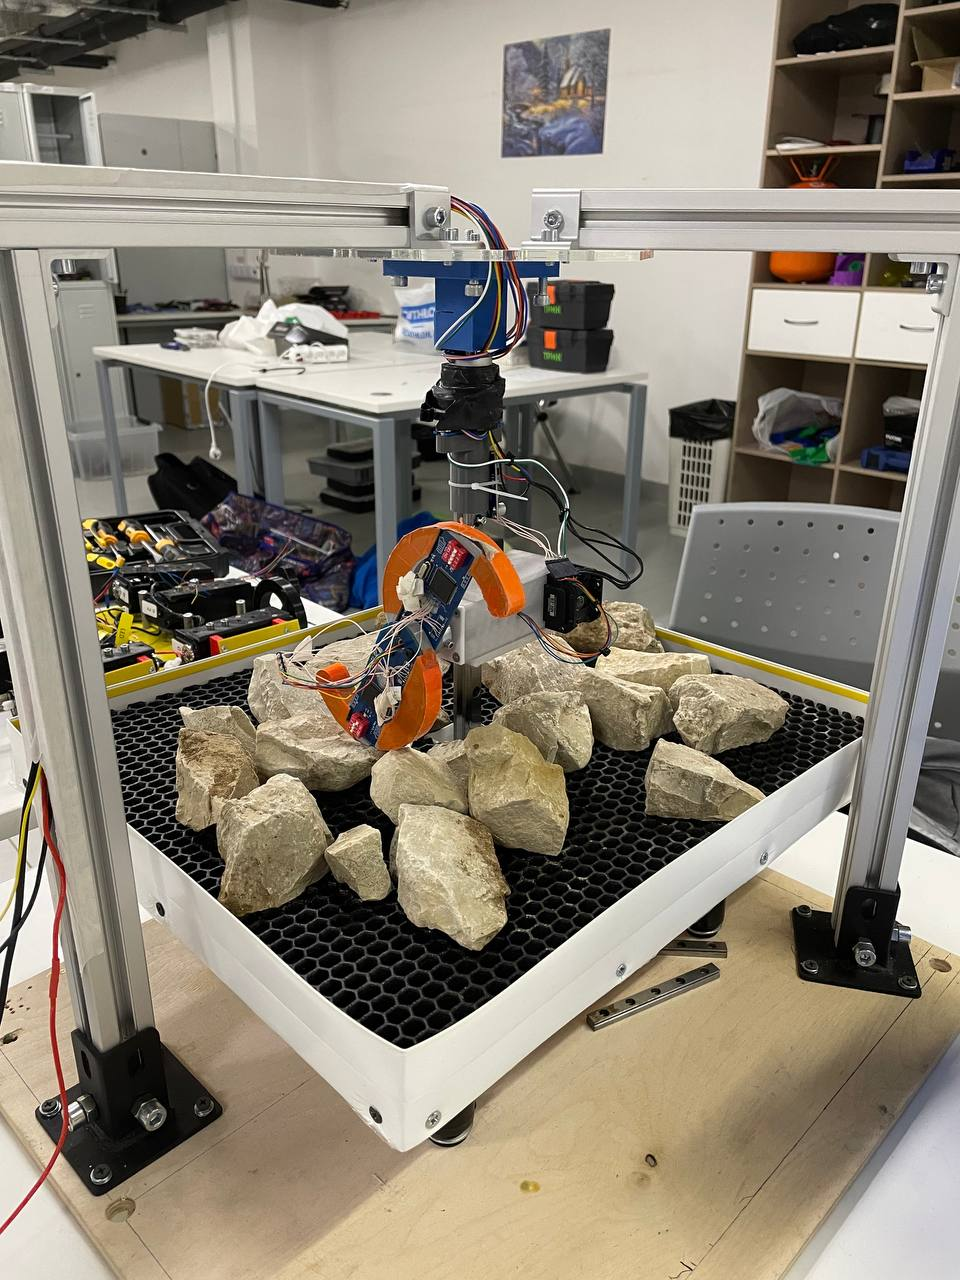
\includegraphics[height=6cm,width=1\textwidth,keepaspectratio]{s_shape_leg/view.jpg}}
            % \caption*{8mm end-effector diam}
        \end{subfigure}
    \end{figure}
\end{frame}

% \begin{frame}[t]{Определение типа поверхности}
%     \framesubtitle{Velostat transducer properties}
%     \large
%     \begin{itemize}
%         \item Because of high hysteresis and difficulties with calibration, we have to work with relative data.
%     \end{itemize}
% \end{frame}

\begin{frame}[t]{Определение типа поверхности}
    \framesubtitle{Данные с одного эксперимента}
    \begin{columns}[T,onlytextwidth]
        \begin{column}{0.60\textwidth}
            \begin{figure}[H]
                \centering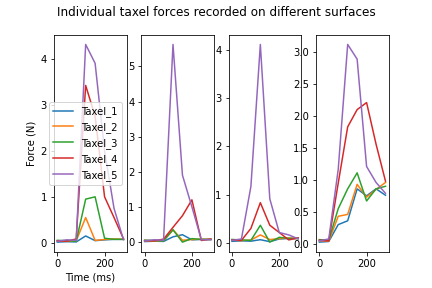
\includegraphics[height=5cm,width=1\textwidth,keepaspectratio]{s_shape_leg/TaxelIndForce.png}
            \end{figure}
        \end{column}
        \begin{column}{0.35\textwidth}
            \vspace{-1.6cm}
            \begin{figure}[H]
                \begin{subfigure}{0.99\textwidth}
                    \centering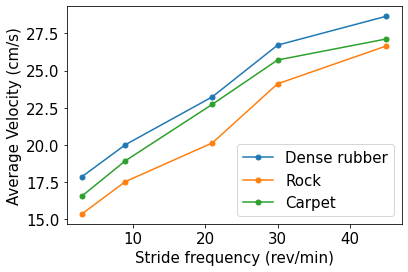
\includegraphics[height=3.8cm,width=1\textwidth,keepaspectratio]{s_shape_leg/avg_lin_vel_rev_min.png} 
                \end{subfigure}

                \begin{subfigure}{0.99\textwidth}
                    \centering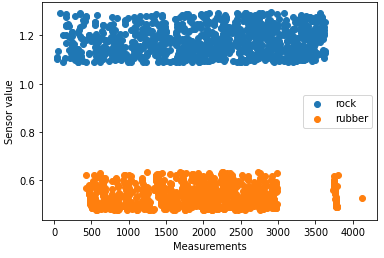
\includegraphics[height=3.8cm,width=1\textwidth,keepaspectratio]{s_shape_leg/segment6_compare_front.png}
                \end{subfigure}
                

            \end{figure}
        \end{column}
    \end{columns}
\end{frame}

\begin{frame}[t]{Определение типа поверхности}
    \framesubtitle{Итог}
    \large
    \begin{itemize}
        \item Возможность различать резиновую и каменистую поверхность.
        \item Выбраны параметры классификации рельефа для машинного обучения:
              \begin{itemize}
                \large
                  \item Число оборотов в минуту
                  \item Крутящий момент двигателя
                  \item Ускорение от IMU
                  \item Данные о силе, которые представлены как значение датчика\/сегмент, пиковая амплитуда, средняя амплитуда
              \end{itemize}
        \item Velostat датчик силы доказал свою работоспособность.
    \end{itemize}
\end{frame}

\begin{frame}[t]{Картографирование с помощью датчиков силы}
    \framesubtitle{}
    \only<1-2>{\large\begin{block}{Вопрос}
        Как создать плотное облако точек, используя разреженные данные об точках касания ног?
        \end{block}}
    \only<2>{\large\begin{alertblock}{Ответ}
            \centering \textit{Создать полигональную сетку}, используя 2D триангуляцию Делоне (вогнутая оболочка) с использованием разреженных данных, \textit{сгенерировать новые точки} и вернуть данные навигации
        \end{alertblock}}
\end{frame}

\begin{frame}[t]{Картографирование с помощью датчиков силы}
    \framesubtitle{Места проведения экспериментов}
    \vspace{-15pt}
    \begin{figure}[H]
        \begin{subfigure}[t]{0.49\textwidth}
            \centering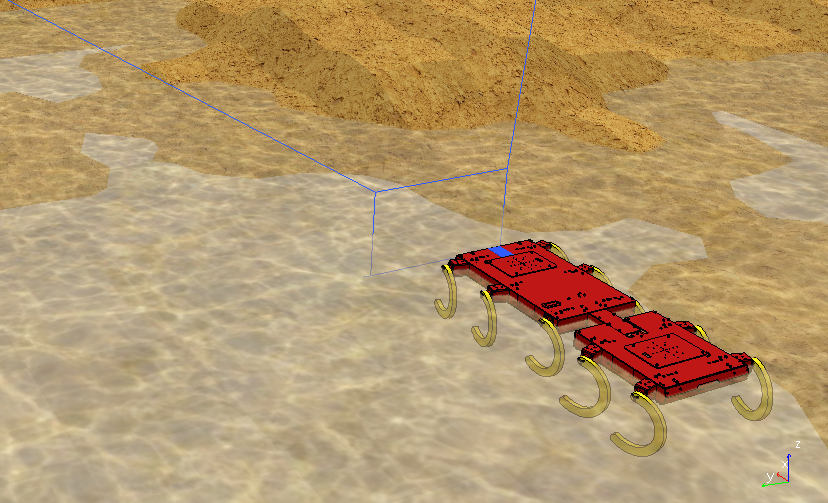
\includegraphics[height=5cm,width=1\textwidth,keepaspectratio]{coppelia_sim.png}
            \caption*{CoppeliaSim симулятор,\\ \textbf{4th gen} СтриРус}
        \end{subfigure}
        \begin{subfigure}[t]{0.49\textwidth}
            \centering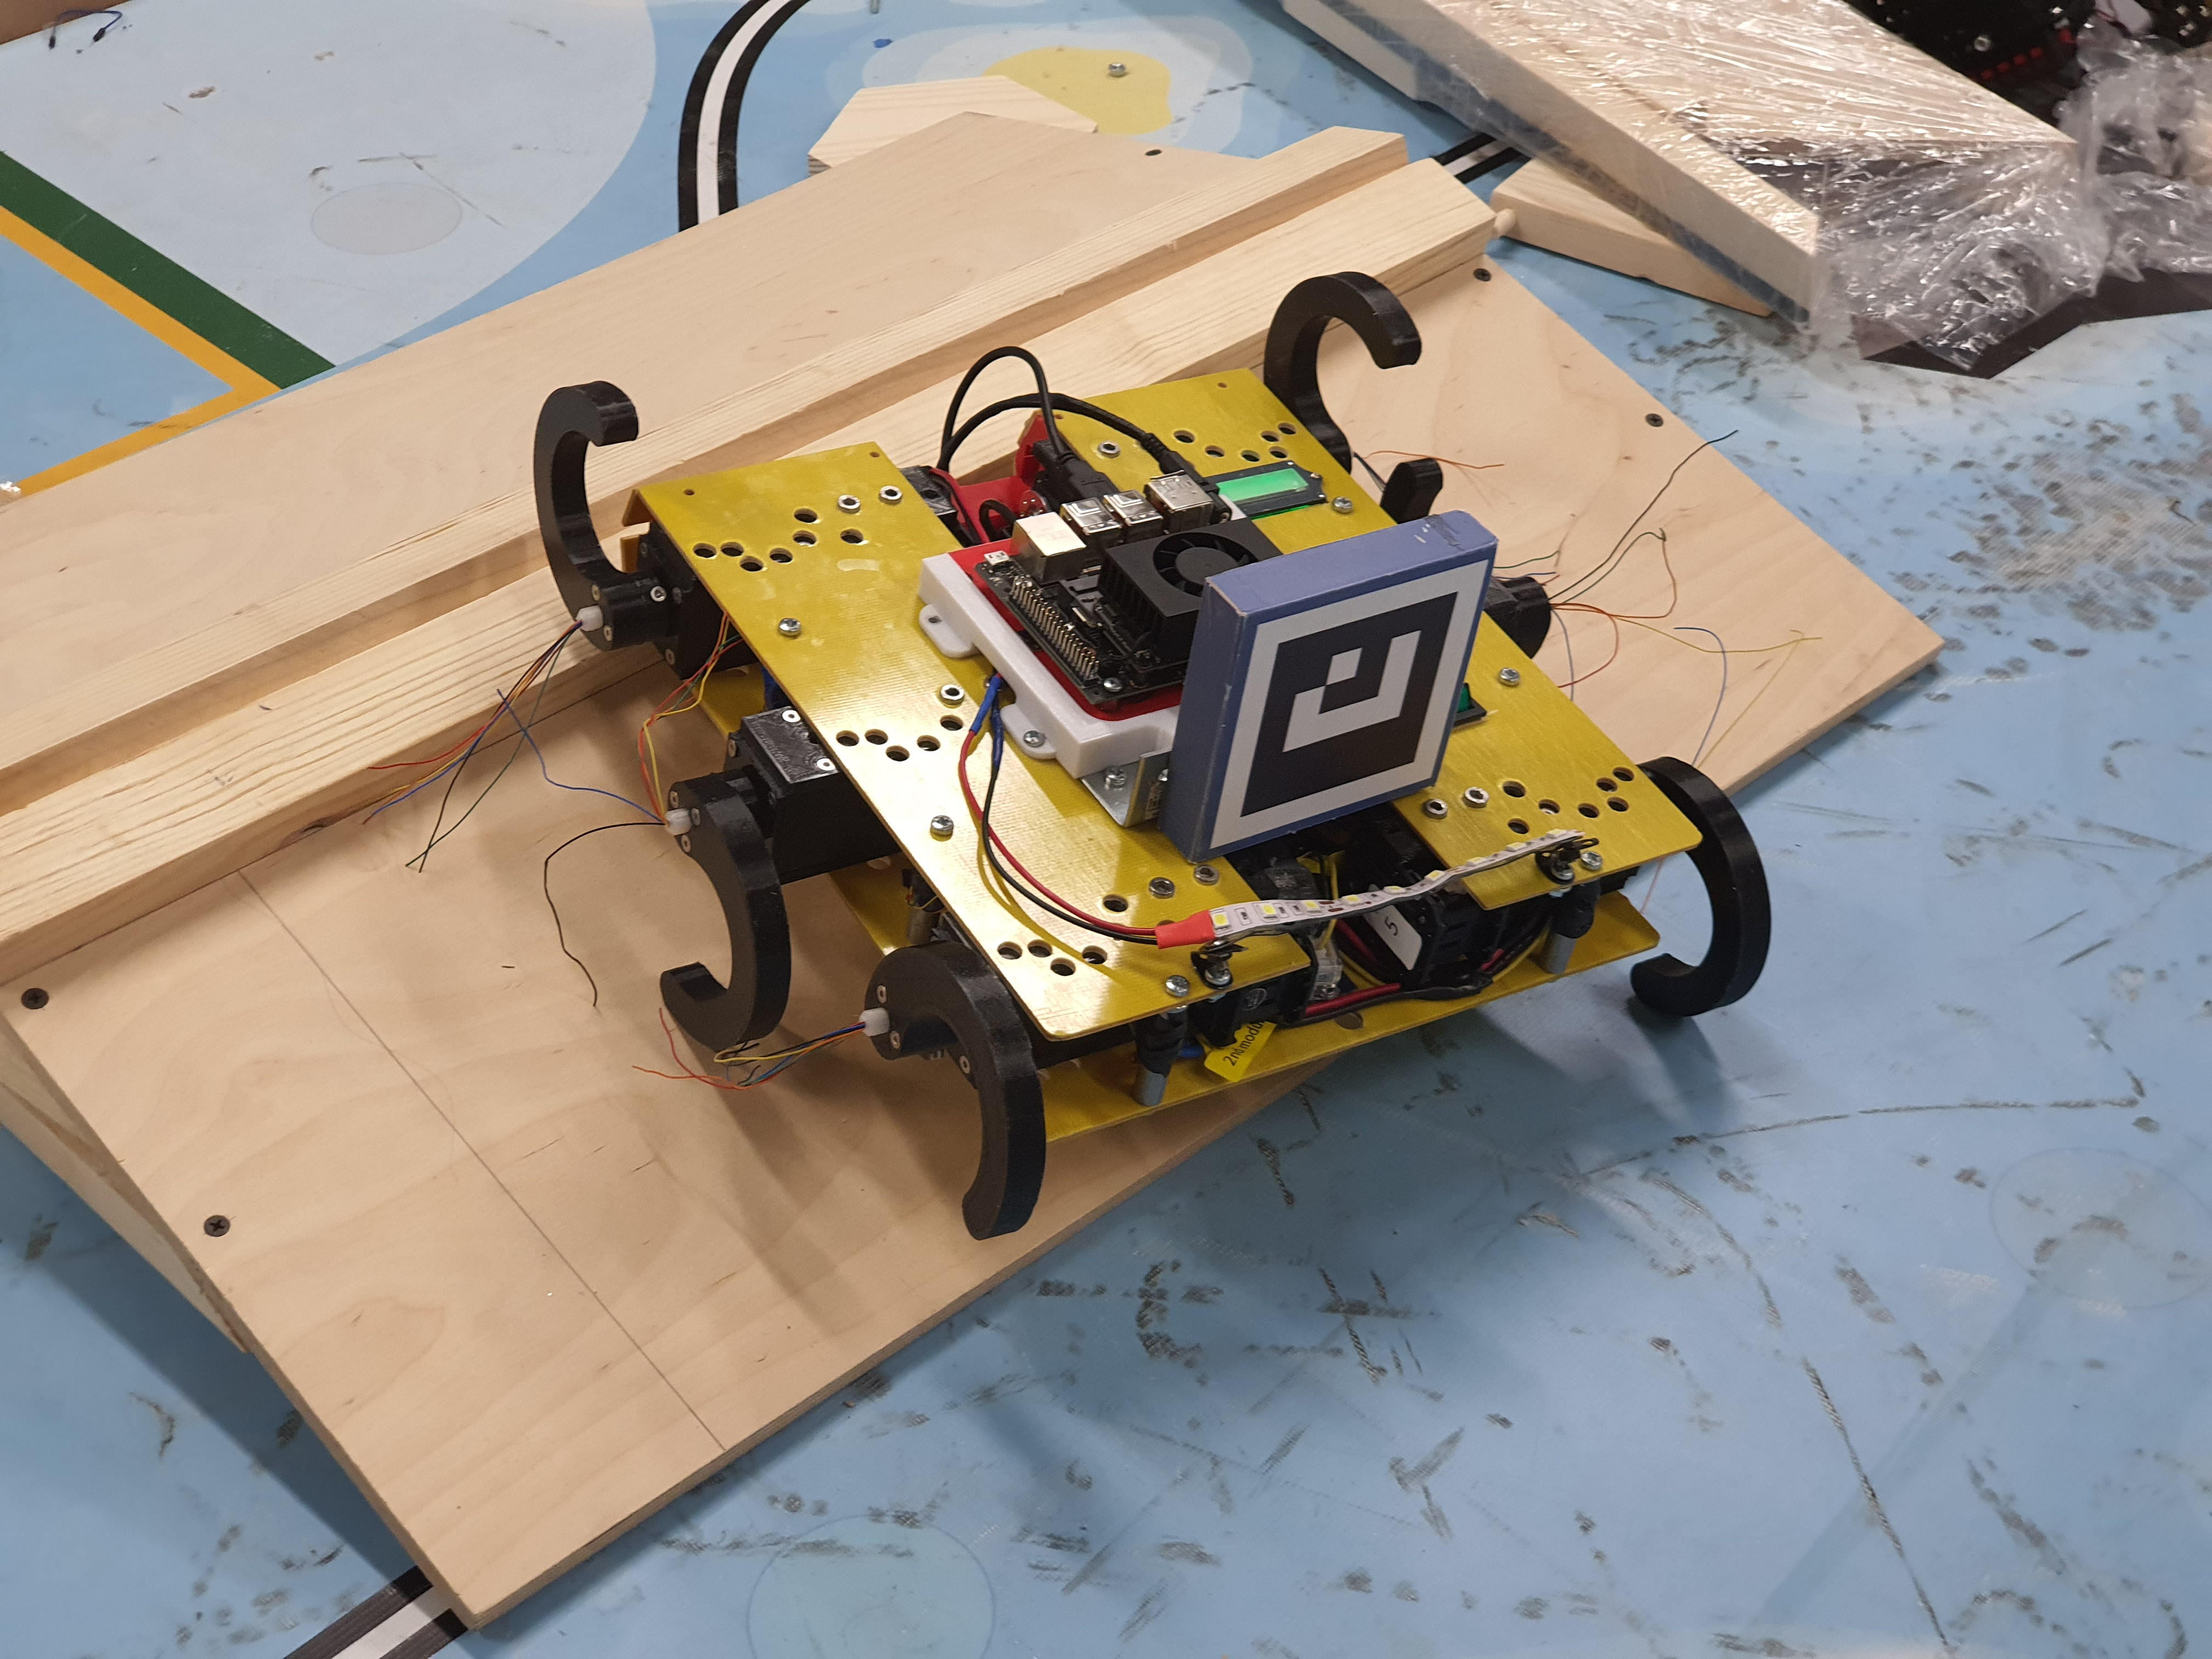
\includegraphics[height=5cm,width=1\textwidth,keepaspectratio]{rl_sim.JPG}
            \caption*{Натурные испытания,\\ \textbf{3th+ gen} СтриРус}
        \end{subfigure}
    \end{figure}
\end{frame}

\begin{frame}[t]{Картографирование с помощью датчиков силы}
    \framesubtitle{Предположения}
    \large
    Текущее решение с учетом таких предположений:
    \begin{itemize}
        \item Наша местность может быть представлена $z = f(x,y)$. Поэтому используется 2D триангуляция Делоне (проецирование точек на плоскость)
        \item Все данные моделирования предварительно обрабатываются белым шумом
    \end{itemize}
\end{frame}

\begin{frame}[t]{Картографирование с помощью датчиков силы}
    \framesubtitle{Триангуляция Делоне}
    \vspace{-0.2cm}
    \begin{figure}[H]
        \centering\includegraphics[height=6cm,width=1\textwidth,keepaspectratio]{delone_idea.png}
        \caption*{2D триангуляция Делоне (Выпуклая оболочка) \\ \textbf{От облака точек к полигональной сетке}}
        \label{fig:delone_idea.png}
    \end{figure}
\end{frame}

\begin{frame}[t]{Картографирование с помощью датчиков силы}
    \framesubtitle{Результат: Симулятор, маршрут}
    \vspace{-15pt}
    \begin{figure}[H]
        \begin{subfigure}[t]{0.49\textwidth}
            \centering\includegraphics[height=5cm,width=1\textwidth,keepaspectratio]{terrain_w_water1.png}
            \caption*{Начало маршрута}
        \end{subfigure}
        \begin{subfigure}[t]{0.49\textwidth}
            \centering\includegraphics[height=5cm,width=1\textwidth,keepaspectratio]{terrain_w_water_end.png}
            \caption*{Конец маршрута}
        \end{subfigure}
    \end{figure}
\end{frame}

\begin{frame}[t]{Картографирование с помощью датчиков силы}
    \framesubtitle{Результат: Полигональная сетка и сгенерированные точки}
    \vspace{-15pt}
    \begin{figure}[H]
        \begin{subfigure}[t]{0.49\textwidth}
            \centering\includegraphics[height=5cm,width=1\textwidth,keepaspectratio]{mesh_rviz.png}
            \caption*{Сетка, созданная 2D триангуляциией Делоне (вогнутая оболочка)}
        \end{subfigure}
        \begin{subfigure}[t]{0.49\textwidth}
                \centering
                 \begin{tikzpicture}
                    % Include the image in a node
                    \node [above right, inner sep=0] (image) at (0,0) 
                    {\centering\includegraphics[height=5cm,width=1\textwidth,keepaspectratio]{sampled_pcd.png}};          
                    % Create scope with normalized axes
                    \begin{scope}[
                        x={($ 0.1*(image.south east)$)},
                        y={($ 0.1*(image.north west)$)}]
                        % Grid and axes' labels
                        % \draw[lightgray,step=1] (image.south west) grid (image.north east);
                        % \foreach \x in {0,1,...,10} { \node [below] at (\x,0) {\x}; }
                        % \foreach \y in {0,1,...,10} { \node [left] at (0,\y) {\y};}
             
                        % Labels
                        \draw[stealth-, very thick,green] (3,8) -- (2,8.5);
                        \draw[stealth-, very thick,green] (1,5.5) -- (2,8.5)
                        node[rounded corners=3pt,above,black,fill=white]{\tiny Ground Truth Point Cloud};
             
                        \draw[stealth-, very thick,green] (5.5,3) -- (5.5,8.5)
                        node[rounded corners=3pt,above,black,fill=white]{\tiny Generated Point Cloud};
                    \end{scope}
                \end{tikzpicture}
                \caption*{Наложенные облака точек}
                \label{fig:sampled_pcd.png}
        \end{subfigure}
    \end{figure}
\end{frame}


\begin{frame}[t]{Картографирование с помощью датчиков силы}
    \framesubtitle{Почему важно использовать вогнутую оболочку}
    \vspace{-15pt}
    \begin{figure}[H]
        \begin{subfigure}[t]{0.3\textwidth}
            \centering\includegraphics[height=5cm,width=1\textwidth,keepaspectratio]{convex_terr.png}
            \caption*{Пример поверхности}
            \label{fig:convex_terr.png}
        \end{subfigure}
        \hfill
        \begin{subfigure}[t]{0.33\textwidth}
                \centering
                 \begin{tikzpicture}
                    % Include the image in a node
                    \node [above right, inner sep=0] (image) at (0,0) 
                    {\centering\includegraphics[height=6cm,width=1\textwidth,keepaspectratio]{conv_convex.png}};          
                    % Create scope with normalized axes
                    \begin{scope}[
                        x={($ 0.1*(image.south east)$)},
                        y={($ 0.1*(image.north west)$)}]
                        % Grid and axes' labels
                        % \draw[lightgray,step=1] (image.south west) grid (image.north east);
                        % \foreach \x in {0,1,...,10} { \node [below] at (\x,0) {\x}; }
                        % \foreach \y in {0,1,...,10} { \node [left] at (0,\y) {\y};}
             
                        % Labels
                        \draw[stealth-, very thick,green] (5.2,3.5) -- ++(1,-1)
                        node[rounded corners=3pt,right,black,fill=white]{\tiny Generated mesh};
                        
                        \draw[stealth-, very thick,green] (5.5,5.5) -- (7.4,4)
                        node[rounded corners=3pt,right,black,fill=white]{\tiny Lidar data};
                        
                        
                        \draw[stealth-, very thick,green] (3.4,0.8) -- (5,1);            
                        \draw[stealth-, very thick,green] (3.4,2.6) -- (5,1)
                        node[rounded corners=3pt,right,black,fill=white]{\tiny Cloud of contact points};
                    \end{scope}
                \end{tikzpicture}
                \caption*{Выпуклая оболочка}
                \label{fig:conv_convex.png}
        \end{subfigure}
        \hfill
        \begin{subfigure}[t]{0.33\textwidth}
            \centering\includegraphics[height=6cm,width=1\textwidth,keepaspectratio]{conv_concave.png}
            \caption*{Вогнутая оболочка}
            \label{fig:conv_concave.png}
        \end{subfigure}

    \end{figure}
\end{frame}

\begin{frame}[t]{Картографирование с помощью датчиков силы}
    \framesubtitle{Метрика C2C: Сравнение эталонного и полученного облаков точек}
    \vspace{-15pt}
    \begin{figure}[H]
        \begin{subfigure}[t]{0.49\textwidth}
            \centering\includegraphics[height=5cm,width=1\textwidth,keepaspectratio]{cropped_pcd.png}
            \caption*{Наложенные облака точек}
        \end{subfigure}
        \begin{subfigure}[t]{0.49\textwidth}
            \centering\includegraphics[height=5cm,width=1\textwidth,keepaspectratio]{pcd_hist.png}
            \caption*{Гистограмма ошибок (расстояние от точки до ближайшей эталонной)}
        \end{subfigure}
    \end{figure}
    % \alert{\large RMSE 0.053074, std 0.025}
\end{frame}

\begin{frame}[t]{Картографирование с помощью датчиков силы}
    \framesubtitle{Метрика C2M: Сравнение эталонной и полученной сеток}
    \vspace{-15pt}
    \begin{figure}[H]
        \begin{subfigure}[t]{0.49\textwidth}
            \centering\includegraphics[height=5cm,width=1\textwidth,keepaspectratio]{mesh_comp.png}
            \caption*{Наложенные сетки}
        \end{subfigure}
        \begin{subfigure}[t]{0.49\textwidth}
            \centering\includegraphics[height=5cm,width=1\textwidth,keepaspectratio]{mesh_hist.png}
            \caption*{Гистограмма ошибок (расстояние от точки до ближайшей эталонной)}
        \end{subfigure}
    \end{figure}
    % \alert{\large RMSE 0.00167067, std 0.0005}
\end{frame}

\begin{frame}[t]{Картографирование с помощью датчиков силы}
    \framesubtitle{Результат: Натурные испытания, Видео}
    \vspace{-0.5cm}
    \begin{figure}[H]
        \begin{subfigure}[t]{0.49\textwidth}
            % \href{run:./videos/big_angle2.mp4}{
            \href{https://youtu.be/2dxHHTG4psQ}{
                \centering\includegraphics[height=6cm,width=1\textwidth,keepaspectratio]{real_robot_mesh_video_preview.png}}
            \caption*{Робот проходит препятствие}
        \end{subfigure}
        \begin{subfigure}[t]{0.49\textwidth}
            \centering\includegraphics[height=6cm,width=1\textwidth,keepaspectratio]{real_mesh.jpg}
            \caption*{Полигональная сетка, полученная с помощью ног}
        \end{subfigure}
    \end{figure}
\end{frame}

\begin{frame}[t]{Картографирование с помощью датчиков силы}
    \framesubtitle{Итог}
    \large
    \begin{itemize}
        \item Карта может быть построена с помощью \textit{вогнутой оболочки 2D триангуляции Делоне}, где входными данными являются \textit{точки касания, определенные датчиком силы}.
        \item \textit{Симулятор} (Среднее значение среднеквадратичной ошибки): \begin{itemize}
            \large
                  \item При сравнении облаков точек составляет около 5 см.
                  \item При сравнении сеткок составляет около 1 см.
              \end{itemize}
        \item \textit{Натурный эксперимент} (---//---): \begin{itemize}
            \large
                  \item При сравнении облаков точек составляет около 8 см.
                        % \item Среднее значение. RMSE при сравнении сетки составляет около 1 см.
              \end{itemize}
              \textit{Это приемлимая точность для такой задачи.}
    \end{itemize}
\end{frame}


\begin{frame}[t]{Глобальный итог}
    \framesubtitle{}
    \large
    \vspace{-0.5cm}
    \begin{figure}[H]
        \begin{subfigure}[t]{0.49\textwidth}
            \centering\includegraphics[height=2.5cm,width=1\textwidth,keepaspectratio]{strirus_3.JPG}
            \caption*{1. Структурный синтез}
        \end{subfigure}
        \begin{subfigure}[t]{0.49\textwidth}
            \centering\includegraphics[height=2.5cm,width=1\textwidth,keepaspectratio]{velostat_sensor_look.JPG}
            \caption*{2. Датчик силы на основе Velostat}
        \end{subfigure}
    
        \begin{subfigure}[t]{0.49\textwidth}
            \centering\includegraphics[height=2.5cm,width=1\textwidth,keepaspectratio]{s_shape_leg/s_leg_setup.JPG}
            \caption*{3. Определение поверхности}
        \end{subfigure}
        \begin{subfigure}[t]{0.49\textwidth}
            \centering\includegraphics[height=2.5cm,width=1\textwidth,keepaspectratio]{conv_concave.png}
            \caption*{4. Ножное картографирование}
        \end{subfigure}
    \end{figure}
\end{frame}

% \fbckg{fibeamer/figs/last_page.png}
% \frame[plain]{}
% \fbckg{fibeamer/figs/common.png}

\end{document}